\documentclass[12pt]{article}
\usepackage[italian]{babel}
\usepackage{graphicx}
\usepackage[section]{placeins}
\usepackage{amsmath}
\usepackage{amsfonts} 
\usepackage{enumitem}
\usepackage{listings}
\usepackage{hyperref}
\usepackage{tcolorbox}
\usepackage[ruled, italiano, linesnumbered]{algorithm2e}
\usepackage{caption}
\usepackage{subcaption}
\usepackage{tikz}
\usepackage{xcolor,listings}
\usepackage{textcomp}
\usepackage{color}

\definecolor{codegreen}{rgb}{0,0.6,0}
\definecolor{codegray}{rgb}{0.5,0.5,0.5}
\definecolor{codepurple}{HTML}{C42043}
\definecolor{backcolour}{HTML}{F2F2F2}
\definecolor{bookColor}{cmyk}{0,0,0,0.90}  
\color{bookColor}

\lstset{upquote=true}

\lstdefinestyle{mystyle}{
    backgroundcolor=\color{backcolour},   
    commentstyle=\color{codegreen},
    keywordstyle=\color{codepurple},
    numberstyle=\footnotesize\color{codegray},
    stringstyle=\color{codepurple},
    basicstyle=\footnotesize,
    breakatwhitespace=false,         
    breaklines=true,                 
    captionpos=b,                    
    keepspaces=true,                 
    numbers=left,                    
    numbersep=-10pt,                  
    showspaces=false,                
    showstringspaces=false,
    showtabs=false,      
}
\lstset{style=mystyle} 

\bibliographystyle{plain}

\tcbuselibrary{theorems}
\newtcbtheorem[number within = section]{definition}{\emph{Defionizione}}{colback = gray!10, colframe = gray!50!black, fonttitle = \bfseries}{th}
\newtcbtheorem[]{theorem}{\emph{Theorem }}{colback = gray!10, colframe = gray!50!black, fonttitle = \bfseries}{th}

\title{Progetto di Geospatial Data Management}
\author{
\begin{tabular}[t]{c@{\extracolsep{6em}}c} 
Giuseppe Maurizio Facchi  & Gregorio Ghidoli \\
mat. 989910 & mat. 983827\\ 
\end{tabular}
}

\date{A.A. 2021-2022}

\begin{document}

\maketitle

\newpage
\tableofcontents

\newpage
\section{Introduzione}
Il progetto del corso di Geospatial Data Management dell'anno accademico 2021-2022 è volto a familiarizzare con l'analisi di traiettorie, un tipo di dato spazio-temporale.
In particolare, sono state fornite tre traiettorie percorse all'interno di un museo da tre diverse persone, con l'obiettivo di:
\begin{enumerate}
    \item trovare i punti di fermata delle persone;
    \item per ogni persona, calcolare per quanto tempo ha osservato ciascuna esibizione del museo, considerando solo i punti di fermata;
    \item per ogni esibizione del museo, calcolarne il tempo totale di osservazione, considerando solo i punti di fermata delle persone nei loro pressi;
    \item per ogni esibizione del museo, trovare il numero di persone che la osservano congiuntamente nel tempo.
\end{enumerate}

\section{Concetti generali}
Prima di presentare il lavoro svolto per il progetto, introduciamo i concetti generali che possono aiutare a capire e a trattare il problema proposto.\\
L’operazione relativa all’estrazione di informazioni che arricchiscono la conoscenza
del dominio di un problema prende il nome di \emph{data mining}. Una possibile
organizzazione delle operazioni presenti in letteratura nel caso del paradigma del \emph{trajectory data mining}, ovvero l'estrazione di informazioni dalle traiettorie, è specificata nella Figura \ref{trajectorydatamining}.
\begin{figure}
    \centering
    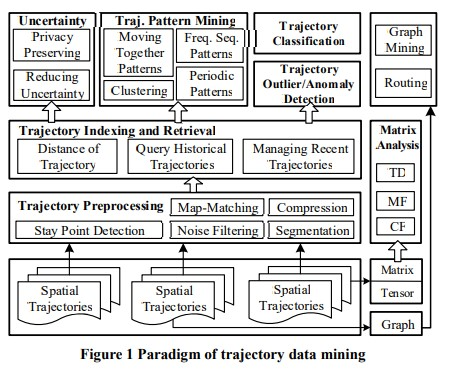
\includegraphics[width=0.6\textwidth]{images/datamining.jpg}
    \caption{Paradigma del trajectory data mining descritto in \cite{TrajectoryDataMining}. Nella Figura sono evidenziate le fasi affrontate per lo svolgimento del progetto.}
    \label{trajectorydatamining}
\end{figure}
\begin{definition}{Traiettoria}{}
    Una traiettoria rappresenta il movimento, ovvero l'evoluzione della posizione nel tempo, di un oggetto nel mondo reale (persona, animale, automobile, ecc...), detto anche \emph{moving object}, in uno spazio geografico durante un dato intervallo di tempo.
    Tipicamente, una traiettoria viene rappresentata e memorizzata come una sequenza di punti cronologicamente ordinati $$p_1 \rightarrow p_2 \rightarrow \dots \rightarrow p_n,$$ dove ogni punto consiste in una coppia di coordinate geografiche associate ad un timestamp $$p_i=(x_i,y_i,t_i), i=0,\dots,n,x_i,y_i,t_i \in \mathbb{N}.$$
\end{definition}
Durante una traiettoria, il moving object può non cambiare la sua posizione, o cambiarla leggermente, per un determinato periodo di tempo, caratterizzando un punto di fermata.
\begin{definition}{Punto di fermata - Stop Point}{}
    Viene generalmente definito "punto di fermata", un punto nel dominio spazio-temporale dove un'entità risulta essere stazionaria. Esistono tipicamente due condizioni di stazionarietà:
    \begin{itemize}
        \item l'entità rimane ferma nello stesso punto per un certo periodo di tempo;
        \item definita un'area, l'entità rimane all'interno di essa per un certo periodo di tempo.
    \end{itemize}
    Dunque, visualizzando le traiettorie come sequenze di punti, i punti di fermata possono essere identificati da un gran numero di punti sparpagliati attorno a una posizione, oppure come un unico punto a cui è assegnato un elevato intervallo di tempo rispetto ai successivi.
    \label{stop_point}
\end{definition}
Questo comporamento è utile da individuare all'interno di una traiettoria in quanto può rappresentare un'attività importante svolta dal moving object, come fermarsi in un posto per mangiare o, nel caso di questo progetto, visitare un'esibizione di un museo.
Da questa osservazione si può quindi pensare di estrarre dalla traiettoria le sequenze di movimento e le sequenze di fermata (\emph{stop}) tramite operazioni di \emph{preprocessing}, come \emph{stay point detection} e \emph{trajectory segmentation}.
In questo modo si passa da una visione “piatta” della traietttoria a una visione arrichita di informazioni, ovvero le sequenze di movimento e di fermata, utili per future analisi o processi di \emph{trajectory pattern mining}, come individuare punti di interesse o comportamenti di affollamento.
\begin{definition}{Sequenza}{}
    Una sequenza è qualsiasi serie continua di punti in una traiettoria.
\end{definition}
Tipicamente, le sequenze di movimento sono caratterizzate dal fatto che il moving object mantiene una velocità relativamente sostenuta coprendo distanze relativamente lunghe in brevi intervalli di tempo, mentre nelle sequenze di stop mentiene velocità molto basse, anche pari a zero, coprendo distanze molto brevi in intervalli di tempo relativamente lunghi
\footnote{Nelle analisi bisogna fare attenzione a non identificare come sequenze di stop le sequenze in cui il movimento è molto lento ma scorrevole (lineare) o fermate momentanee di brevissima durata.}.\\
Tuttavia, l'inevitabile presenza di rumore all'interno dei dati spazio-temporali relativi a traiettorie complica l'estrazione di sequenze significative e l'analisi di queste ultime.
Il rumore è dovuto a errori di misurazione e di campionamento nei sistemi di acquisizione di dati spazio-temporali, chiamati sistemi RLTS, e porta ad avere una deviazione dei punti della traiettoria dalla reale posizione del moving object.
\begin{definition}{Rumore della traiettoria - Noise}{}
    Il rumore della traiettoria (\emph{noise}) è la deviazione dei punti di una traiettoria dalla posizione reale del moving object, dovuta a errori di misurazione e campionamento.
\end{definition}
\begin{definition}{Real-Time Location System - RTLS}{}
    Si definisce Real-Time Location System (RTLS) qualsiasi sistema, hardware e software, in grado di campionare accuratamente ad alta frequenza la posizione di un'entità in uno spazio definito.\\
    Gli RTLS forniscono la posizione di un tag e, in base alle loro caratteristiche, una posizione può indicare:
    \begin{itemize}
        \item la \text{presenza} in un'area, espressa simbolicamente;
        \item la \text{posizione precisa}, espressa in coordinate;
        \item la \text{vicinanza} ad un altro tag, espressa come distanza o in modo simbolico.
    \end{itemize}
    Quando l'entità di cui si acquisisce la posizione partecipa direttamente all'attività di tracciamento tramite l'utilizzo di RTLS, allora si parla di \textbf{registrazione attiva}.
\end{definition}
Per l'estrazione di sequenze di stop, nel progetto abbiamo codificato e utilizzato tre algoritmi proposti in letteratura e che seguono approcci diversi:
\begin{itemize}
    \item un algoritmo basato su \emph{time-space threshold} (\emph{PMLH}), presentato in \cite{SpaceTimeTreshold};
    \item un algoritmo di clustering di sequenze (\emph{SOC}) \footnote{Sebbene il clustering sia una tecnica di data mining, in questo progetto viene usato come tecnica di preprocessing per l'estrazione di sequenze di stop.}, presentato in \cite{SequenceClustering};
    \item un algoritmo basato su un approccio statistico (\emph{MSN}), presentato in \cite{Statistical}.
\end{itemize}

\section{Analisi del dataset}
Il dataset fornito contiene le traiettorie percorse all'interno di un museo da tre diversi visitatori, la cui posizione è stata registrata attivamente per un intervallo di tempo di circa 10 minuti ad una frequenza di compionamento di circa $12Hz$.
In aggiunta, sono stati forniti due shapefile ESRI contenenti rispettivamente le geometrie dei tavoli del museo e le geometrie delle esposizioni.
La posizione dei punti tracciati e delle geometrie è rappresentata secondo l'ESPG 3003.
Per visualizzare i tavoli, le esibizioni e le traiettorie abbiamo utilizzato QGIS, ottenendo la Figura \ref{tables_with_exhibits} e la Figura \ref{tables_with_exhibits_and_trajectories}.

\begin{figure}[htb!]
    \centering
    \begin{subfigure}[b]{0.4\textwidth}
        \centering
        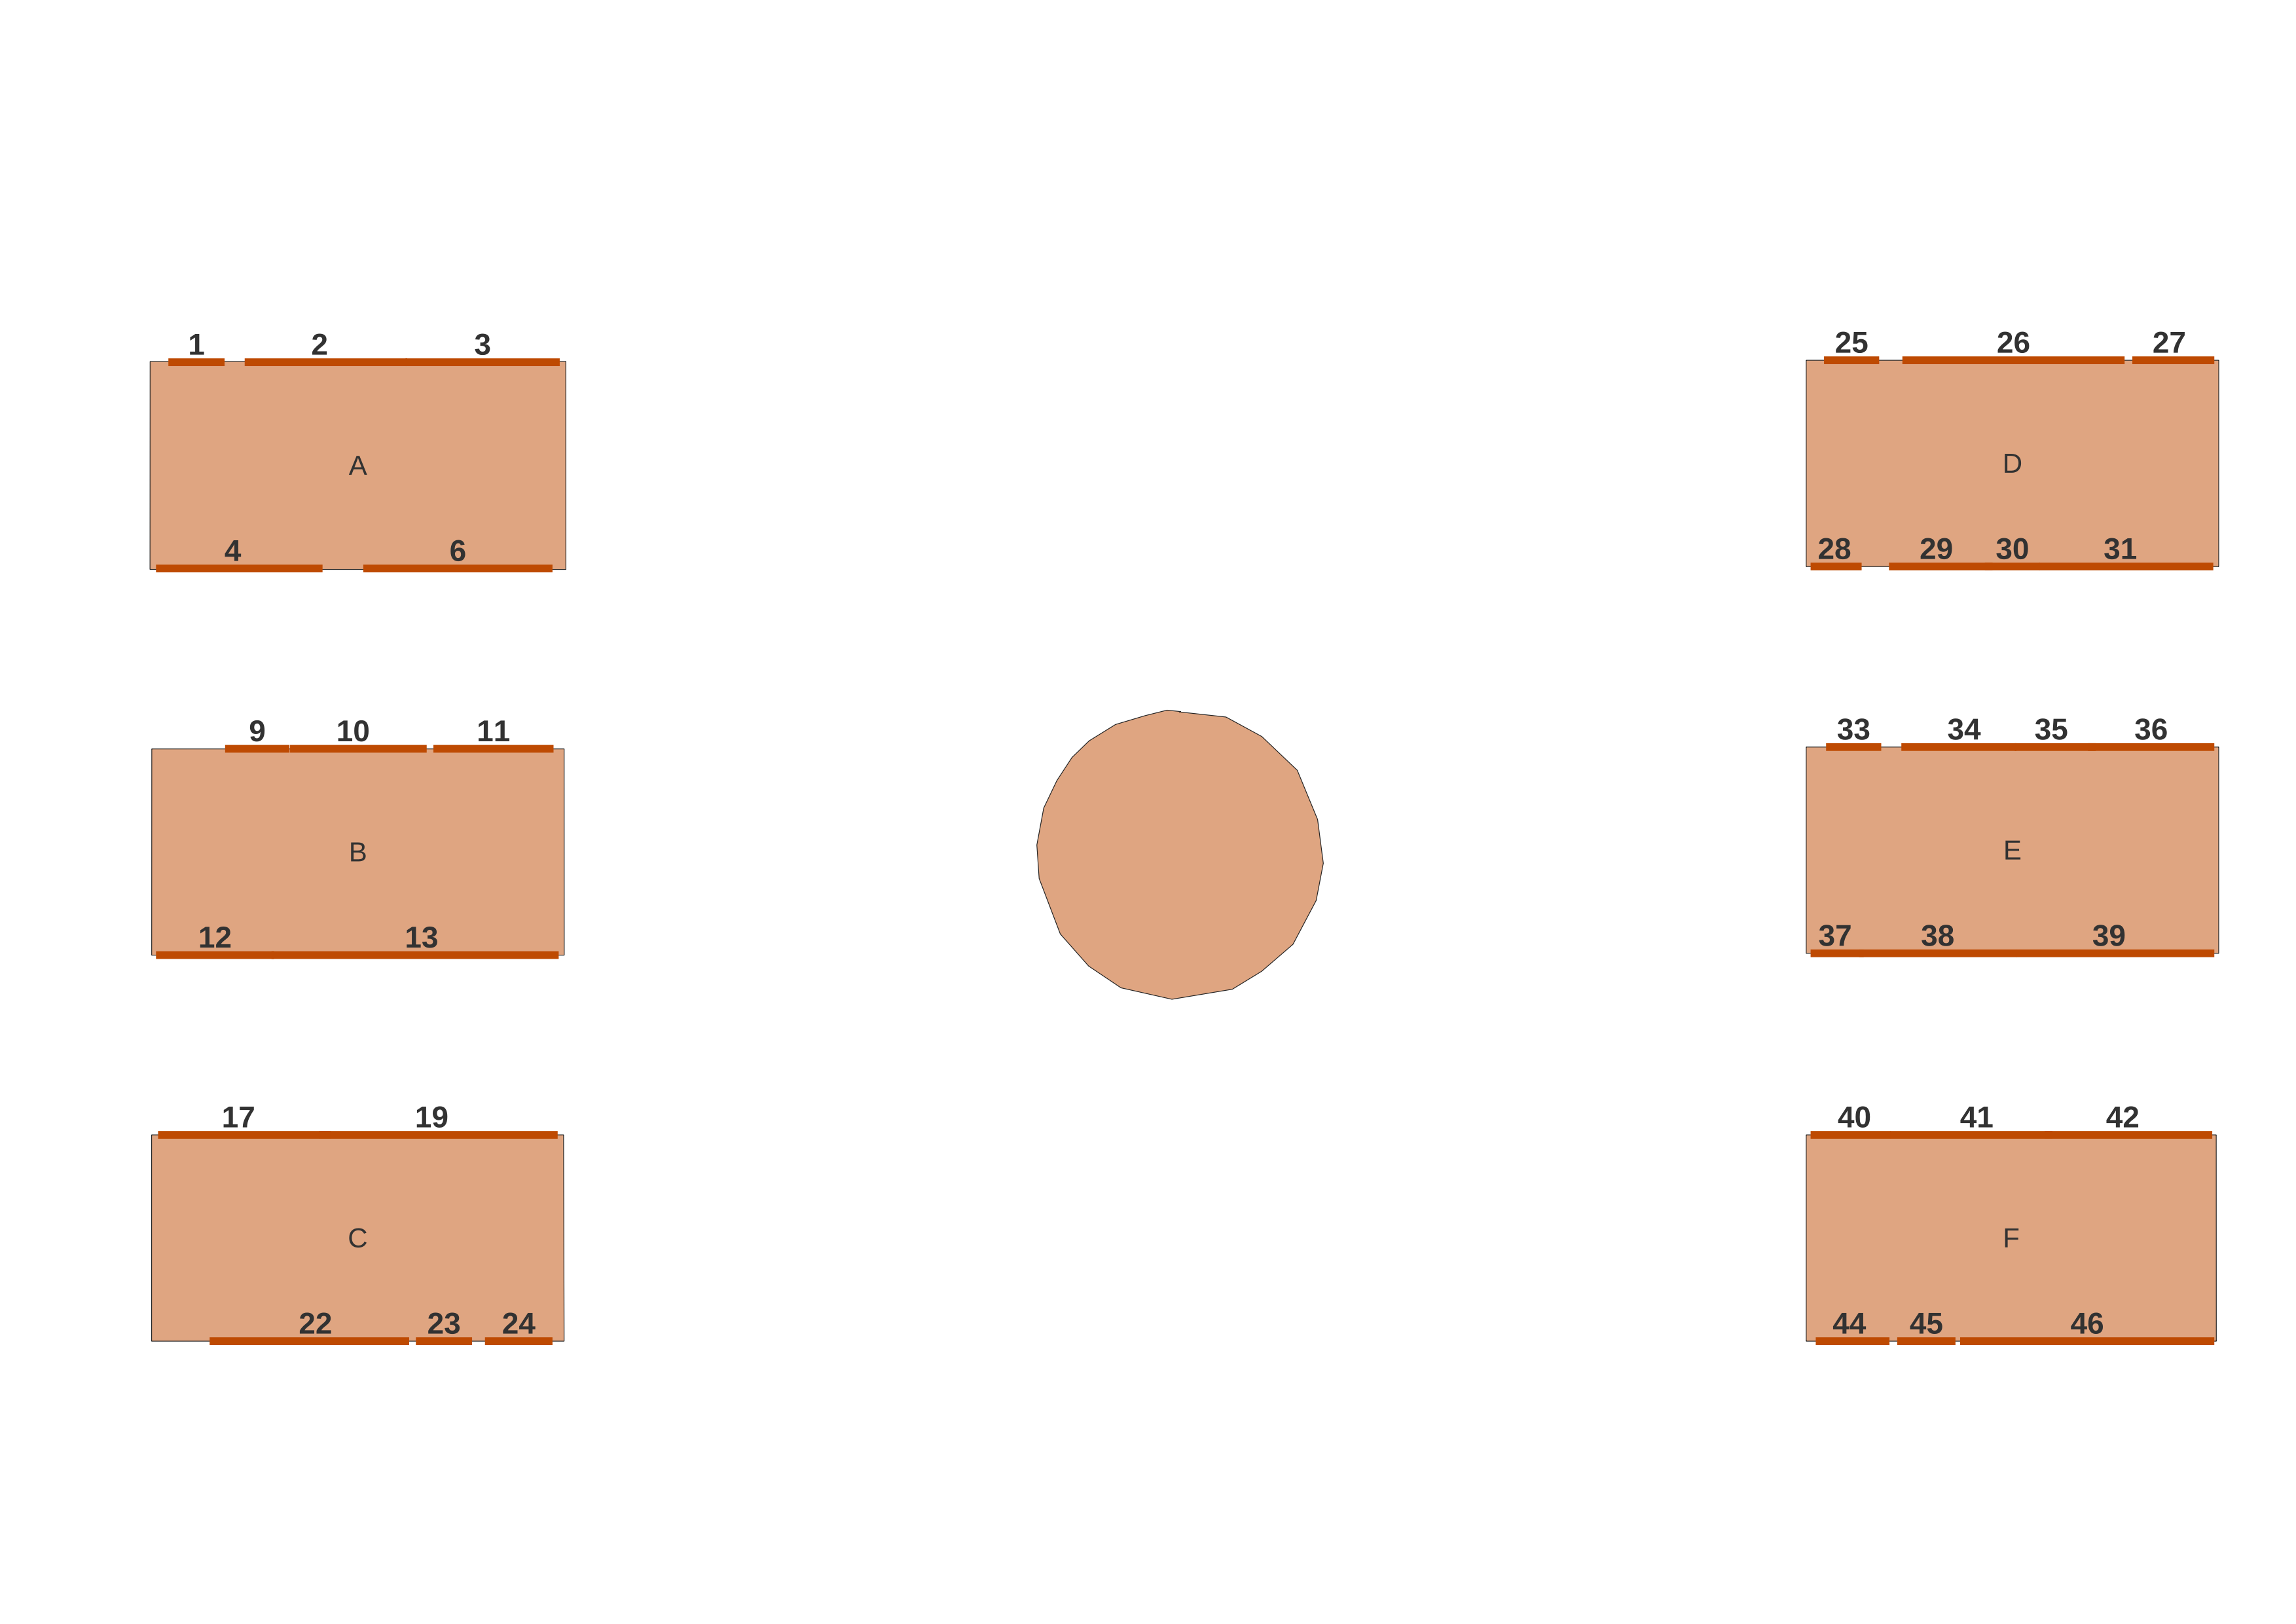
\includegraphics[width=\textwidth]{images/tables_with_exhibits.png}
        \caption{Tavoli del museo con le esposizioni numerate.}
        \label{tables_with_exhibits}
    \end{subfigure}
    \hfill
    \begin{subfigure}[b]{0.4\textwidth}
        \centering
        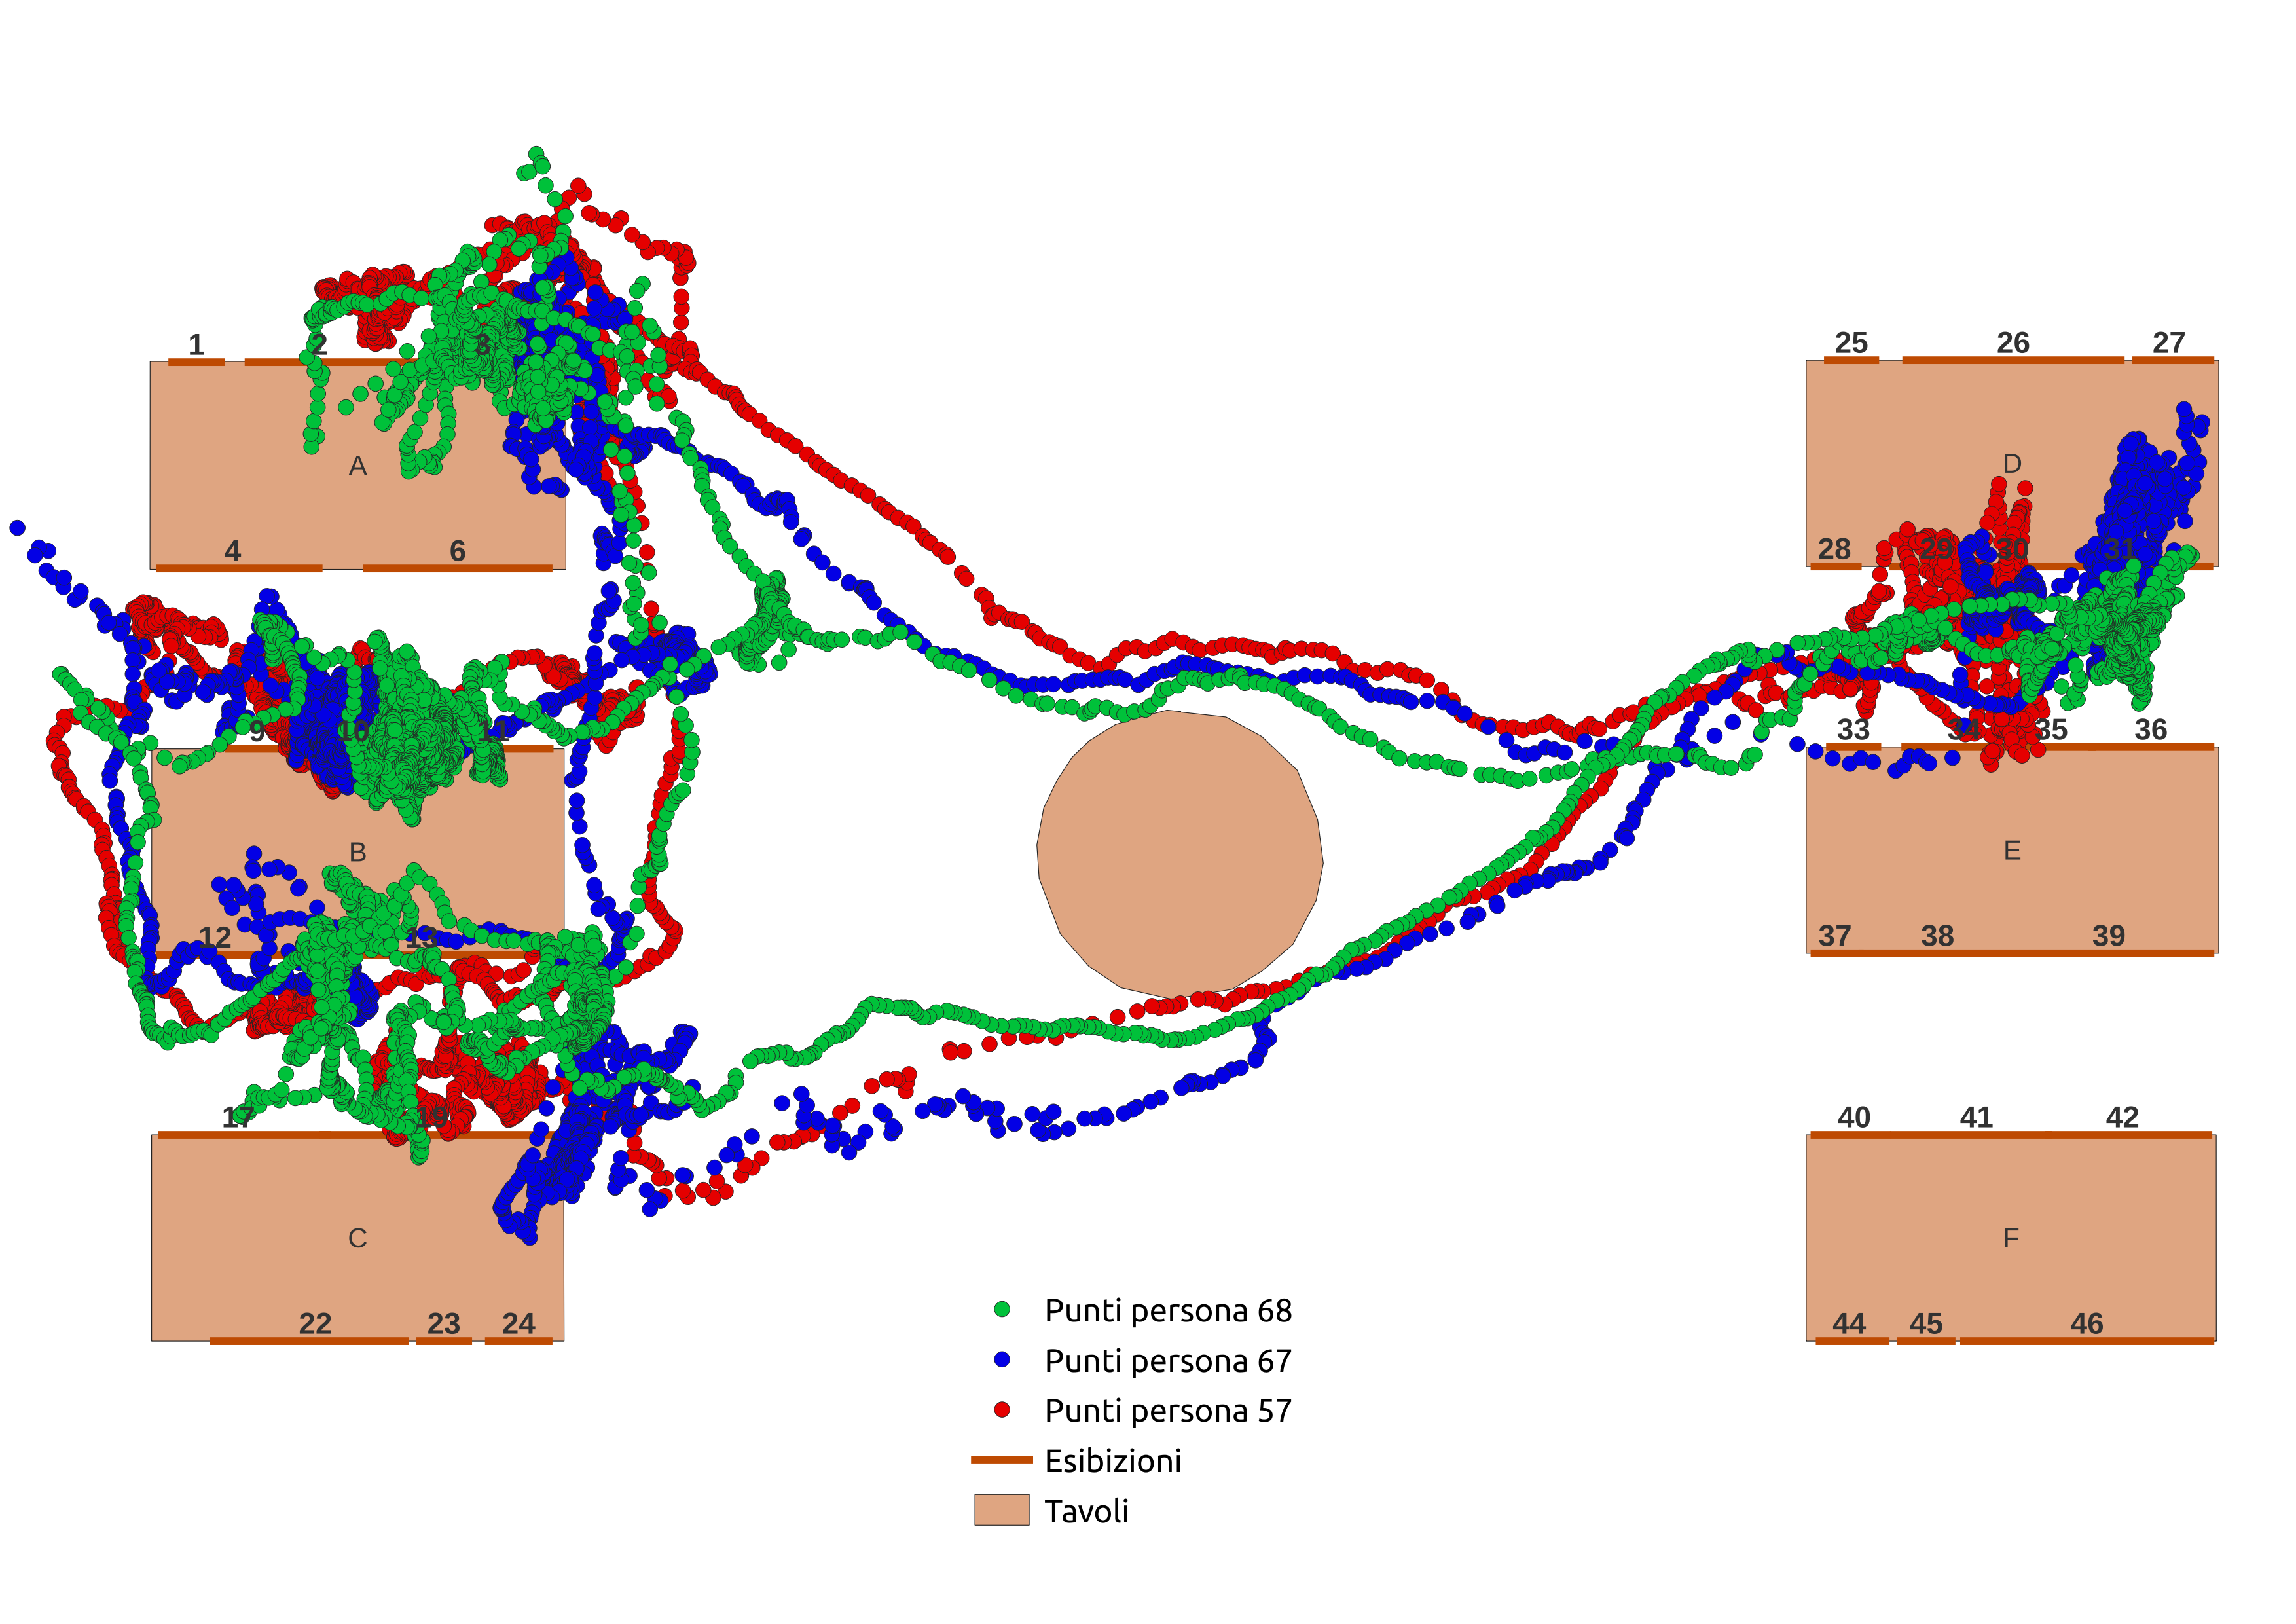
\includegraphics[width=\textwidth]{images/tables_with_exhibits_and_trajectories.png}
        \caption{Traiettorie rappresentate come sequenze di punti.}
        \label{tables_with_exhibits_and_trajectories}
    \end{subfigure}
    \hfill
    \caption{}
\end{figure}

Per ottenere una rappresentazione succinta delle traiettorie abbiamo calcolato le statistiche contenute nella Tabella \ref{trajectories_aggregates_informations}.
Ci siamo serviti di questi dati aggregati principalmente per avere una linea guida su come impostare i parametri degli algoritimi utilizzati.

\begin{table}[!ht]
    \centering
    \begin{tabular}{cccc}
        \multicolumn{4}{c}{\textit{\textbf{Persona 57}}}                                                                                                                \\ \cline{2-4}
        \multicolumn{1}{c|}{}                  & \multicolumn{1}{c|}{\textbf{Distanza}} & \multicolumn{1}{c|}{\textbf{Durata}} & \multicolumn{1}{c|}{\textbf{Velocità}} \\ \hline
        \multicolumn{1}{|c|}{\textbf{Media}}   & \multicolumn{1}{c|}{0.0403}            & \multicolumn{1}{c|}{0.085}           & \multicolumn{1}{c|}{0.4852}            \\ \hline
        \multicolumn{1}{|c|}{\textbf{Mediana}} & \multicolumn{1}{c|}{0.0307}            & \multicolumn{1}{c|}{0.072}           & \multicolumn{1}{c|}{0.3743}            \\ \hline
        \multicolumn{1}{|c|}{\textbf{Minimo}}  & \multicolumn{1}{c|}{0.0002}            & \multicolumn{1}{c|}{0.071}           & \multicolumn{1}{c|}{0.0022}            \\ \hline
        \multicolumn{1}{|c|}{\textbf{Massimo}} & \multicolumn{1}{c|}{0.5754}            & \multicolumn{1}{c|}{0.179}           & \multicolumn{1}{c|}{4.1787}            \\ \hline
                                               &                                        &                                      &                                        \\
        \multicolumn{4}{c}{\textit{\textbf{Persona 67}}}                                                                                                                \\ \cline{2-4}
        \multicolumn{1}{c|}{}                  & \multicolumn{1}{c|}{\textbf{Distanza}} & \multicolumn{1}{c|}{\textbf{Durata}} & \multicolumn{1}{c|}{\textbf{Velocità}} \\ \hline
        \multicolumn{1}{|c|}{\textbf{Media}}   & \multicolumn{1}{c|}{0.052}             & \multicolumn{1}{c|}{0.089}           & \multicolumn{1}{c|}{0.6134}            \\ \hline
        \multicolumn{1}{|c|}{\textbf{Mediana}} & \multicolumn{1}{c|}{0.0389}            & \multicolumn{1}{c|}{0.072}           & \multicolumn{1}{c|}{0.454}             \\ \hline
        \multicolumn{1}{|c|}{\textbf{Minimo}}  & \multicolumn{1}{c|}{0.0006}            & \multicolumn{1}{c|}{0.071}           & \multicolumn{1}{c|}{0.003}             \\ \hline
        \multicolumn{1}{|c|}{\textbf{Massimo}} & \multicolumn{1}{c|}{0.4939}            & \multicolumn{1}{c|}{0.179}           & \multicolumn{1}{c|}{6.2258}            \\ \hline
                                               &                                        &                                      &                                        \\
        \multicolumn{4}{c}{\textit{\textbf{Persona 68}}}                                                                                                                \\ \cline{2-4}
        \multicolumn{1}{c|}{}                  & \multicolumn{1}{c|}{\textbf{Distanza}} & \multicolumn{1}{c|}{\textbf{Durata}} & \multicolumn{1}{c|}{\textbf{Velocità}} \\ \hline
        \multicolumn{1}{|c|}{\textbf{Media}}   & \multicolumn{1}{c|}{0.0454}            & \multicolumn{1}{c|}{0.088}           & \multicolumn{1}{c|}{0.5456}            \\ \hline
        \multicolumn{1}{|c|}{\textbf{Mediana}} & \multicolumn{1}{c|}{0.0343}            & \multicolumn{1}{c|}{0.072}           & \multicolumn{1}{c|}{0.4169}            \\ \hline
        \multicolumn{1}{|c|}{\textbf{Minimo}}  & \multicolumn{1}{c|}{0.0008}            & \multicolumn{1}{c|}{0.071}           & \multicolumn{1}{c|}{0.0108}            \\ \hline
        \multicolumn{1}{|c|}{\textbf{Massimo}} & \multicolumn{1}{c|}{0.7911}            & \multicolumn{1}{c|}{5.356}           & \multicolumn{1}{c|}{10.9884}           \\ \hline
    \end{tabular}
    \caption{Statistiche relative alle traiettorie dei visitatori.}
    \label{trajectories_aggregates_informations}
\end{table}

\section{Individuazione dei punti di fermata}
Al giorno d'oggi, grazie alla diffusione di dispositivi come i ricevitori GPS, si hanno a disposizione grandi quantità di dati relativi a traiettorie.
Questo tipo di dati è utilizzato in diversi ambiti di ricerca, quali lo studio della mobilità personale, la gestione del trasporto urbano e l'analisi del comportamento umano e animale.
Al fine di studiare al meglio questi problemi, è utile individuare accuratamente informazioni semantiche sulle traiettorie originali, come le sequenze di movimento e di fermata.
Come descritto in \cite{ReviewMethods}, le tecniche per l'estrazione di sequenze di stop presenti in letteratura si divono in tre classi: metodi basati su \emph{time-distance threshold}, algoritmi di clustering basati sulla densità e metodi basati su approcci statistici.
Sono ancora ambito di ricerca i nuovi approcci, ad esempio \cite{ReviewMethods}, che considerano gli elementi geografici in prossimità delle traiettorie, tra i quali figurano i \emph{point of interest} (POI), per un'estrazione delle sequenze più precisa.
Per questo progetto abbiamo implementato e sperimentato l'utilizzo di tre algoritmi, ciascuno appartenente a una delle diverse categorie. Dopo aver confrontato i risultati, abbiamo deciso di proseguire le analisi con gli esiti dell'algoritmo di clustering.

\subsection{Algoritmo basato su time-space threshold}
In \cite{SpaceTimeTreshold} viene descritto l'Algoritmo \ref{PMLH}, da noi identificato come PMLH, appartenente alla categoria dei metodi basati su time-space threshold.
PMLH, infatti, considera solamente la dimensione spaziale e temporale delle traiettorie, senza prenedere in considerazione altri eventuali parametri, come la velocità del moving object, o l'inevitabile presenza di rumore nei dati.
L'algoritmo identifica sequenze continue di punti che rimangono entro una certa distanza per almeno un periodo di tempo fissato .
La funzione \emph{diameter} calcola la distanza più grande tra ogni elemento di un insieme, mentre la funzione \emph{memoid} identifica la posizione del punto in una sequenza che minimizza la massima distanza da ogni altro punto della stessa, ovvero il punto più vicino al centro della sequenza.
L'algoritmo restituisce un insieme di tuple  $s_i=(seq_i, t_i^{start}, t_i^{end})$. Partendo da questo insieme è facile classificare i punti della traiettoria secondo la loro appartenenza o meno alle fermate identificate dai memoidi $seq_i$, verificando che il timestamp di un punto sia compreso tra $t_i^{start}$ e $t_i^{end}$.

\paragraph{Descrizione dei parametri}
\begin{itemize}
    \item  Roaming distance, $\Delta l_{roam}$: rappresenta la massima distanza a cui un punto $p_i$ può stare da un altro punto $p_j$ per poter essere considerato come facente parte della fermata di $p_j$;
    \item  Stay duration, $\Delta t_{dur}$: rappresenta la minima durata per cui il moving object deve stare entro la roaming distance di un punto $p$ per poter considerare il punto $p$ come facente parte di una fermata.
\end{itemize}
\paragraph{Complessità computazionale} La complessità computazionale di PMLH è $O(n^2)$, dove $n$ è il numero di punti che compongono la traiettoria.\\

\begin{algorithm}
    \caption{PMLH}\label{PMLH}
    \KwData{$trajPoints = \{p_1, \dots p_n\}, \Delta l_{roam}, \Delta t_{dur} $}
    \KwResult{$S = \{s_1,\dots,s_k\}$, $s_i=(seq_i, t_i^{start}, t_i^{end})$ dove $seq_i$ è una sequenza in $trajPoints$}
    $i = 0, S = \emptyset$\;
    \While{$i<|trajPoints|$}{
        $j^* = \min j\;s.t.\;p_j \ge p_i + \Delta t_{dur}$\;
        \eIf{$diameter(i,j*) > \Delta l_{roam}$}
        {$i = i + 1$\;}
        {$j^* = \max j\;s.t.\;diameter(i, j) \le \Delta l_{roam}$\;
            $S = S \cup (medoid (i, j^*), t_i, t_{j^*})$\;
            $i = j^* + 1$\;}
    }
\end{algorithm}

\subsection{Algoritmo di clustering di sequenze}
In letteratura sono presenti diversi metodi per la segmentazione di traiettorie che identificano i punti o le sequenze di stop facendo considerazioni sul cambio di profilo della velocità e della direzione del moving object quando questo passa da uno stato di movimento a uno stato di fermata.
Un'altro approccio per affrontare il problema consiste nell'uso di tecniche di data-mining, come gli algoritmi di clustering basati sulla densità dove, tra quelli specializzati per i dati spazio-temporali, si annoverano CB-SMoT, T-OPTICS e TrajDBSCAN.
Tuttavia, questi approcci non forniscono buoni risultati quando si ha un elevato rumore nei dati e, inoltre, non determinano come fermate i singoli punti, chiamati \emph{big point}, a cui è associato un elevato intervallo di tempo.
Un buon algoritmo di clustering deve ridurre il più possibile la creazione di veri negativi, come le sequenze di stop non individuate o le sequenze di stop separate dal rumore, e il numero di falsi positivi, come le sequenze di movimento molto lento e di forma lineare, cercando quindi di incrementare il rapporto di sequenze di stop effettive individuate.
A questo proposito è stato proposto l'algoritmo Sequence Oriented Clustering (SOC), descritto in \cite{SequenceClustering}, che permette di determinare i punti di rumore come facenti parte delle sequenze di stop, queste aventi forma arbitraria, e di individuare i big point.\\\\
SOC è basato su altri due algoritmi di clustering basati sulla densità: DBSCAN e OPTICS, dove quest'ultimo è una generalizzazione del primo.
DBSCAN, come la sua estensione ST-DBSCAN per il clustering di dati spazio-temporali, forma i cluster basandosi sulla nozione di \emph{density-reachability}.
Un punto $p$ è chiamato \emph{core-point} se il vicinato di $p$ contiene un numero $minPts$ di altri punti entro un dato raggio \emph{eps}.
Un punto $q$ si dice \emph{directly density-reachable} da $p$ se $q$ è nel vicinato di $p$.
Un punto $q$ si dice \emph{density-reachable} da $p$ se $q$ è collegato a $p$ da una catena di punti tale per cui ciascun punto è \emph{directly density-reachable} al successivo.
DBSCAN scansiona ciascun punto $p$ una volta e, se $p$ è un core-point, viene creato un nuovo cluster.
Il cluster viene poi espanso ricorsivamente aggiungendo i punti density-reachable dai punti già appartenenti al cluster.\\
Mentre DBSCAN si basa su singoli core-point, l'algoritmo SOC è orientato al clustering di sequenze.
Dall'osservazione che una fermata è costituita da punti tra loro vicini nello spazio e che questi coprono un intervallo temporale relativamente lungo, SOC estrae le sequenze di fermata all'interno di una traiettoria basandosi sul concetto di \emph{core-sequence}: sequenza in cui il moving object rimane in un'area piccola per un lungo periodo di tempo.
Una \emph{eps-sequence} di un punto $p$ è la massima sequenza che contiene $p$ e in cui la distanza (euclidea) tra $p$ e tutti gli altri punti della sequenza è minore di un valore \emph{eps} fissato: $eps$ è il raggio di un'area circolare.
Una \emph{core-sequence} è una sequenza che contiene un punto $p$ per cui la sequenza è una eps-sequence di $p$ e l'intervallo temporale della sequenza è maggiore o uguale a un valore \emph{tau} fissato: quindi il clustering è basato su una densità che tiene conto sia della prossimità spaziale che della continuità e durata nel tempo.
Un \emph{core-point} è un punto per cui la sua eps-sequence è una core-sequence.
La \emph{core-distance} di un punto $p$ è il minimo raggio $r$ minore di $eps$ tale per cui la r-sequence è una core-sequence se la eps-sequence di $p$ è una core-sequence, altrimenti è un valore UNDEFINED predefinito: rappresenta la vicinanza spaziale di un punto ai suoi vicini considerando il tempo, ad esempio è zero nel caso di un big point.
La \emph{reachability-distance} di un punto $p$ è calcolata come segue:
\begin{enumerate}
    \item si controllano $p$ e i punti che precedono $p$;
    \item si trova il punto $q$ precedente e più prossimo a $p$ nella traiettoria tale per cui $p$ appartiene alla core-sequence di $q$;
    \item se $q$ esiste, allora la reachability-distance è il massimo tra la core distance di $q$ e la distanza tra $p$ e $q$;
    \item se non esiste, allora la reachability-distance è UNDEFINED.
\end{enumerate}
Una \emph{eps-reachability sequence} è una sequenza di punti tale per cui la reachability distance di ciascun punto è minore o uguale di \emph{eps} e la reachability-distance del punto che precede la sequenza nella traiettoria e del punto che segue la sequenza nella traiettoria è maggiore di \emph{eps}.\\
Le eps-reachability sequence rappresentano quindi sequenze che si sovrappongono o si incontrano nel tempo.
Una volta calcolata la reachability-distance di ciascun punto, si possono estrarre le eps-reachability sequence e considerarle come sequenze di stop.
Tuttavia, alcune sequenze di stop successive possono essere state erroneamente interrotte da punti di noise.
Per far fronte a questo problema vengono usati due criteri per confrontare eps-reachability sequence successive e nel caso unirle:
\begin{enumerate}
    \item il primo permette di unire due eps-reachability sequence se queste sono vicine in spazio e separate da un periodo di tempo troppo breve per essere considerato un tempo di movimento ragionevole: si usa un parametro $minMov$ che indica la durata minima di un movimento normale.
    \item il secondo permette di unire due eps-reachability sequence se i convex-hull delle stesse si intersecano e se sono separate da un periodo di tempo troppo breve per essere considerato un tempo di movimento ragionevole.
\end{enumerate}
Applicando questi criteri, una eps-reachability sequence cresce fino a quando nessun'altra sequenza può essere unita \footnote{Quando si uniscono due eps-reachability sequence si aggiungono alla sequenza anche i punti di noise intermedi. La reachability distance di questi nodi viene aggiornata al valore $eps$.}.
Tali sequenze vengono chiamate \emph{Ful-reachability sequence}. Le Ful-reachability sequence possono terminare con punti che non fanno parte della sequenza di stop ma che sono raggiungibili dall'ultimo core-point della Ful-reachability sequence.
In questo caso la Ful-reachability sequence viene potata facendola terminare con un core-point e ottenendo così una sequenza di stop.
SOC è in grado di generare sequenze di stop, quest'ultime di forma arbitraria, tra cui sequenze di forma lineare che non rappresentano una fermata effettiva ma un movimento lento.\\
Come ultimo passo dell'algoritmo, vengono quindi filtrate le sequenze di stop false positive per cui gli indici di \emph{straightness} e \emph{centered-distance} presentati in \cite{SequenceClustering} superano una certa soglia.

\paragraph{Descrizione dei parametri}
\begin{itemize}
    \item $eps$ rappresenta il raggio per definire una core-sequence;
    \item $tau$ rappresenta la durata minima per definire una core-sequence;
    \item UNDEFINED rappresenta un valore di default per la reachability distance dei punti della traiettoria: seguendo quanto descritto in \cite{SequenceClustering} viene impostato a $1.2\times eps$;
    \item $minMov$ rappresenta la minima durata che un movimento deve avere per essere considerato un movimento normale: viene usato per unire le eps-reachability sequence;
    \item le misure di straightness e di centered-distance vengono usate per filtrare i falsi positivi: seguendo quando descritto in \cite{SequenceClustering} vengono impostati ai valori di default, rispettivamente $0.5$ e $2\times eps$.
\end{itemize}
La struttura dei cluster è influenzata dal rapporto $\frac{eps}{tau}$.
Diminuendo il valore di $eps$ si restringono le condizioni per identificare le core-sequence, quindi le eps-reachability sequence diminuiscono in dimensione e in numero.
Per questo motivo è più probabile ottenere meno sequenze false positive ma più sequenze vere negative.
Diminuendo il valore di $tau$ si rilassano le condizioni per identificare le core-sequence, quindi  le eps-reachability sequence aumentano in dimensione e in numero.
Per questo motivo è più probabile ottenere più sequenze false positive ma meno sequenze vere negative.
Tuttavia, dai risultati degli esperimenti in \cite{SequenceClustering}, risulta che $eps$ abbia maggiore influenza di $tau$ sull'identificazione delle sequenze e viene consigliato di impostare questi parametri in modo tale che il rapporto $2\times \frac{eps}{tau}$ assuma valori relativamente piccoli.
Infine, diminuendo il valore di $minMov$ si diminuisce la capacità di unire le eps-reachability sequence.
Il parametro $minMov$ deve essere grande abbastanza da eliminare l'influenza del rumore nelle traiettore, ma non troppo grande per evitare di identificare movimenti curvi come sequenze di stop. In generale, il valore di $minMov$ deve essere incrementato quando si ha un elevato numero di punti con rumore.

\paragraph{Complessità computazionale} La complessità di SOC, come per DBSCAN e OPTICS, è $O(n*log\;n)$, , dove $n$ è il numero di punti che compongono la traiettoria.

\begin{algorithm}
    \caption{SOC}\label{SOC}
    \KwData{$trajPoints, eps, tau, \mathrm{UNDEFINED}, minMov$}
    \KwResult{$stops = \{s_1,\dots,s_k\}$ dove $s_i$ è una sequenza in $trajPoints$}
    $\forall p \in trajPoints\;p.reachability\;distance = \mathrm{UNDEFINED}$\;
    \For{$i=1\;to\;|trajPoints|$}{
        $seq$ = epsSequence($trajPoints, p_i, eps$)\;
        \If{isCoreSequence($seq, tau$)}{
            r = coreDistance($seq$)\;
            \For{$j=i\;to\;|trajPoints|$}{
                $p_j.reachability\;distance = max\{r, distance(p_i,p_j)\}$
            }
        }
    }
    epsReachabilitySeqs = extractSequences()\;
    stops = mergeSequences($minMov$)\;
    pruneStops(stops)\;
    falsePositiveRemove(stops)\;
\end{algorithm}

\subsection{Algoritmo basato su un approccio statistico}
In \cite{SpaceTimeTreshold} viene trattata la segmentazione di traiettorie in segmenti di movimento, di fermata e di rumore, come un problema di identificazione di outlier.
Per l'identificazione degli outlier in serie temporali, gli autori utilizzano la statistica \emph{modified z-score}, rappresentata nell'Equazione \ref{modifiedZScore}.
Le costanti $0.6745$ e $1.4826$ servono per rendere le rispettive statistiche non deviate rispetto alla distribuzione normale.
La scelta di utilizzare il modified z-score è motivata dalle scarse prestazioni delle misure di media e deviazione standard in presenza di outlier.
\begin{equation} \label{modifiedZScore}
    M_i = \frac{0.6745(x_i - \overline{x})}{\mathrm{MAD}},\;\;\mathrm{con}\;\mathrm{MAD} = 1.4826 \times median(Y_i - \widetilde{Y})
\end{equation}
Nell'articolo viene suggerito di trattare come outlier i punti che hanno un modified z-score in valore assoluto più grande di $3.5$ e viene proposto l'Algoritmo MSN \ref{MSN} per la segmentazione di traiettorie in segmenti di movimento, di fermata e di rumore.
Per prima cosa, MSN rileva potenziali punti di rumore che hanno distanze relativamente lunghe.
Successivamente, assume che un singolo angolo acuto nella traiettoria rappresenti un movimento di “tornare indietro”, mentre due angoli acuti consecutivi siano da considerare potenziali segmenti di rumore.
Infine, dopo aver rimosso i punti di rumore, identifica i punti la cui durata è molto lunga e la velocità molto bassa \footnote{L'indice modified z-score dovrebbe essere applicato a dati normalmente distribuiti. Data la natura sbilanciata delle velocità, questa viene normalizzata applicando il logaritmo naturale al fine di ristabilire la simmetria.},  classificandoli come punti di stop \footnote{L'algoritmo non tiene conto che punti successivi con velocità inferiore alla soglia specificata possono rappresentare sequenze di movimento e non sequenze di fermata, ottenendo quindi dei falsi-positivi.}.

\paragraph{Descrizione dei parametri}
\begin{itemize}
    \item $S_\tau, T_\tau, V_\tau, A_\tau$: rappresentano le serie di distanza, durata, velocità e angolo di sterzata, relative ai punti della traiettoria $\tau$;
    \item $\epsilon_s, \epsilon_t, \epsilon_v$: rappresentano le soglie del modified z-score rispettivamente per la distanza, la durata e la velocità;
    \item $\theta$: rappresenta l'angolo minimo di sterzata, usato per migliorare l'identificazione del rumore;
    \item $\rho$: rappresenta i limiti dell'intervallo $[-\rho, \rho)$ da cui vengono estratti casualmente in modo uniforme i valori di jitter da aggiungere ai valori di $T_\tau$ per evitare di avere $MAD=0$.
\end{itemize}
I valori dei parametri consigliati dagli autori sono: $\epsilon_s = 3.5, \epsilon_t = 3.5, \epsilon_v = 3.5, \theta = 45, \rho=0.5$.

\paragraph{Complessità computazionale} La complessità di MSN è $O(n)$, dove $n$ è il numero di punti che compongono la traiettoria.

\begin{algorithm}
    \caption{MSN}\label{MSN}
    \KwData{$S_\tau, T_\tau, V_\tau, A_\tau, \epsilon_s, \epsilon_t, \epsilon_v,\theta, \rho$}
    \KwResult{$move\_indexes$, $stop\_indexes$, $noise\_indexes$}
    $distance\_outliers = [], direction\_outliers = [], duration\_outliers = []$\;
    $M_s = modifiedZScore(S_\tau, MAD_s, \overline{s})$\;
    \For{$i=0\;to\;length(M_s)$}{
    \If{$M_s[i]>\epsilon_s$}{
    Appendi $i$ a $distance\_outliers$\;
    }
    }
    \For{$i=0\;to\;length(A_\tau)$}{
        \If{$A_\tau[i]<\theta\;and\;A_\tau[i+1]<\theta$}{
            Appendi $i$ e $i+1$ a $direction\_outliers$\;
            $i++$
        }
    }
    $noise\_indexes = distance\_outliers \cup direction\_outliers$\;
    $clean\_indexes = \tau \setminus \tau[noise\_indexes]$\;
    $\tau = \tau[clean\_indexes]$\;
    $T_\tau = T_\tau + \rho$\;
    $M_t = modifiedZScore(T_\tau, MAD_t, \overline{t})$\;
    \For{$i=0\;to\;length(M_t)$}{
    \If{$M_t[i] > \epsilon_t$}{
    Appendi $i$ a $duration\_outliers$\;
    }
    }
    $V_\tau = ln\;V_\tau$\;
    $speed\_outliers = []$\;
    $M_v = modifiedZScore(V_\tau, MAD_v, \overline{v})$\;
    \For{$i=0\;to\;length(M_v)$}{
    \If{$M_v[i] < -\epsilon_v$}{
    Appendi $i$ a $speed\_outliers$\;
    }
    }
    $stop\_indexes = duration\_outliers \cap speed\_outliers$\;
    $move\_indexes = clean\_indexes \setminus stop\_outliers$\;
\end{algorithm}

\newpage
\subsection{Esperimenti}
Come accennato in \cite{ReviewMethods}, la difficoltà principale negli algoritmi descritti precedentemente risiede nell'impostare correttamente i valori dei parametri.
Inoltre, i valori di default proposti negli articoli citati fanno riferimento a punti registrati da ricevitori GPS in ambienti outdoor e alcuni di questi vanno quindi adattati al contesto di questo progetto.
Analizzando la Figura \ref{tables_with_exhibits_and_trajectories} si vede come le possibili fermate siano costituite da punti racchiusi in aree circolari con raggio di circa 1 metro.
Per questo motivo, in accordo con la Definizione \ref{stop_point}, abbiamo impostato a $1$ i parametri relativi all'area da considerare per identificare eventuali punti di fermata.
In particolare, abbiamo eseguito i seguenti esperimenti:
\begin{itemize}
    \item esecuzione dell'algoritmo PMLH impostando il parametro $\Delta l_{roam}=1$ e il parametro $\Delta t_{dur} \in \{20,30\}$, ottenendo i risultati in Figura \ref{stop_points_PMLH};
    \item esecuzione dell'algoritmo SOC impostando il parametro $eps=1$, il parametro $tau \in \{20,30\}$ e il parametro $minMov = 0.5$, ottenendo i risultati in Figura \ref{stop_points_SOC};
    \item esecuzione dell'algoritmo MSN impostando il parametro $\epsilon_s = 3*\sigma_{M_{S_\tau}}$, il parametro $\epsilon_t = \sigma_{M_{T_\tau}}$,  il parametro $\epsilon_v = \sigma_{M_{V_\tau}}$, il parametro $\theta=45$ e il parametro $\rho=0.0001$, ottenendo i risultati in Figura \ref{stop_segments_MSN}.
\end{itemize}
PMLH, oltre ad avere una complessità computazionale maggiore di SOC e di MSN, restituisce risultati meno precisi in quanto non tratta minimamente il problema della presenza di rumore nei dati: identifica infatti molte più fermate di SOC, tra le quale ve ne sono molte false positive.
MSN invece, secondo \cite{Statistical}, non è un algoritmo congeniale nel caso in cui i dati vengono campionati a frequenza regolare e non fornisce un risultato adatto per le successive analisi: esegue infatti una segmentazione delle traiettorie e non una classificazione dei punti.
Infine SOC, oltre ad avere una buona complessità computazionale, da riscontro grafico sembra individuare sequenze di stop sensate.
Per questi motivi, abbiamo deciso di proseguire le analisi con i risultati forniti dall'algoritmo SOC eseguito con $tau=20$.
\begin{figure}[htb!]
    \centering
    \begin{subfigure}[b]{0.45\textwidth}
        \centering
        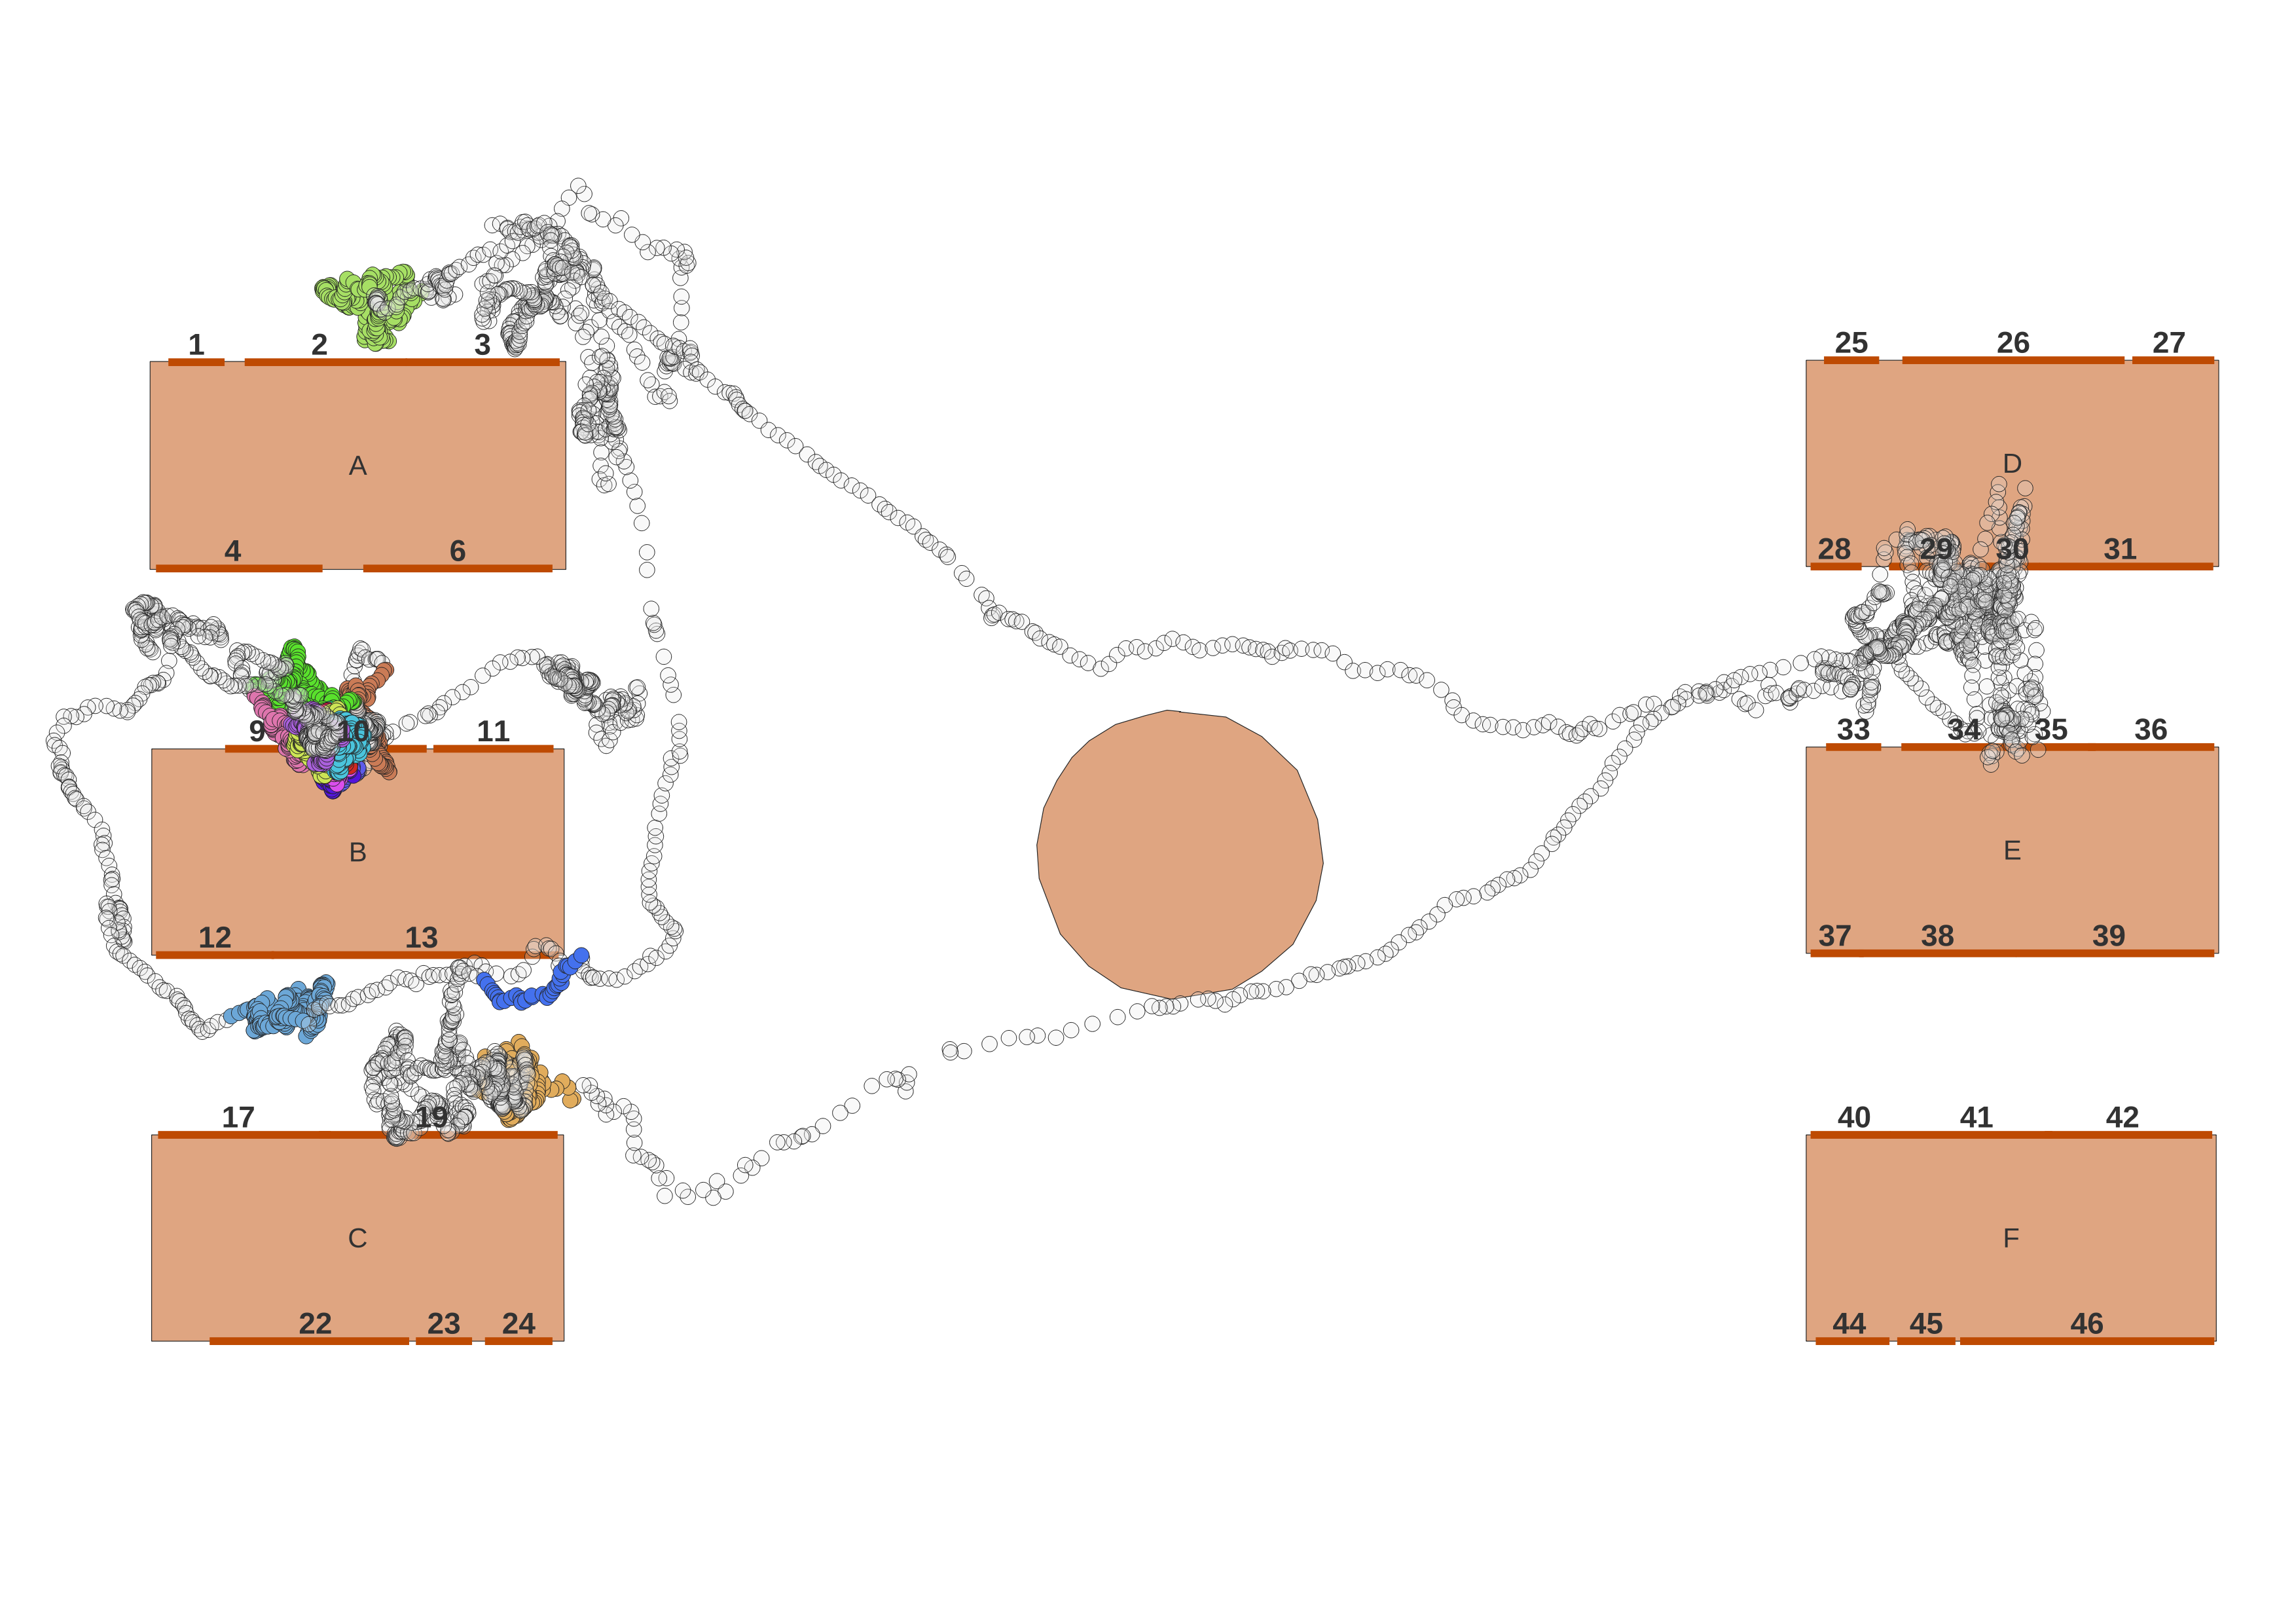
\includegraphics[width=\textwidth]{images/stop_points_p57_PMLH_r1_s20.png}
        \caption{Parametri: $\Delta l_{roam}$=1, $\Delta t_{dur}$=20. Fermate individuate: 19.}
        \label{stop_points_p57_PMLH_r1_s20}
    \end{subfigure}
    \hfill
    \begin{subfigure}[b]{0.45\textwidth}
        \centering
        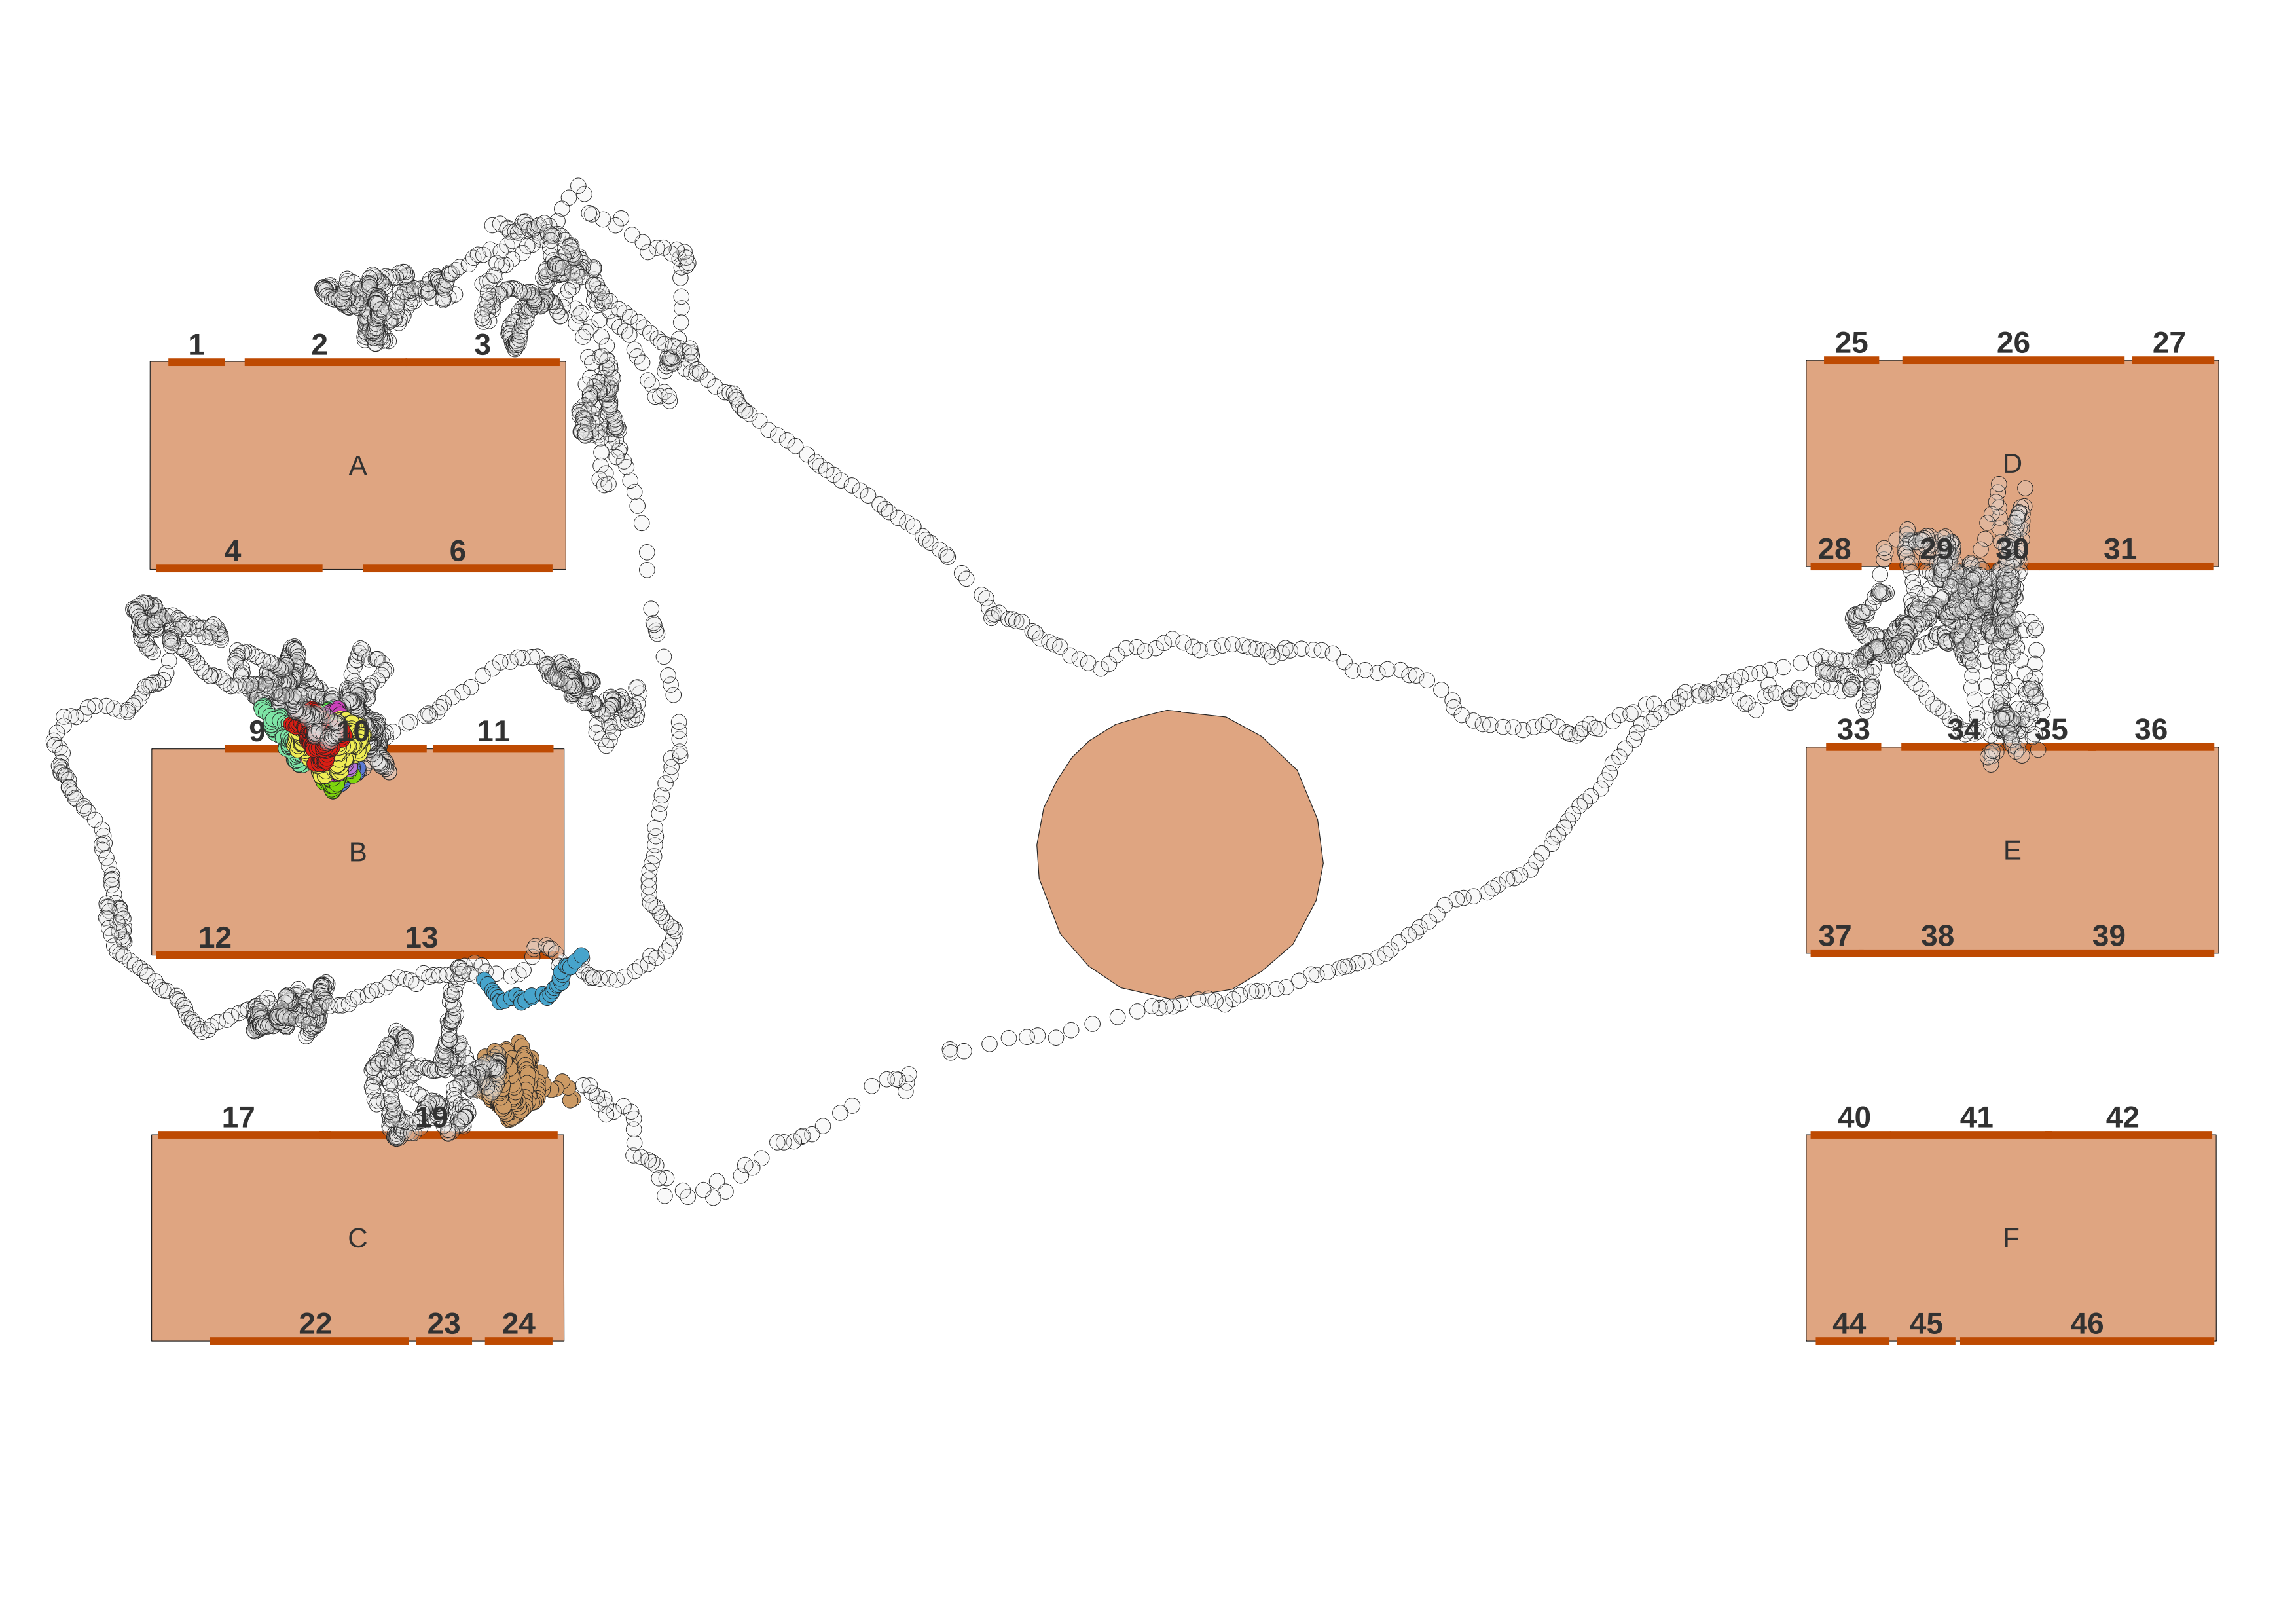
\includegraphics[width=\textwidth]{images/stop_points_p57_PMLH_r1_s30.png}
        \caption{Parametri: $\Delta l_{roam}$=1, $\Delta t_{dur}$=30. Fermate individuate: 11.}
        \label{stop_points_p57_PMLH_r1_s30}
    \end{subfigure}
    \hfill
    \begin{subfigure}[b]{0.45\textwidth}
        \centering
        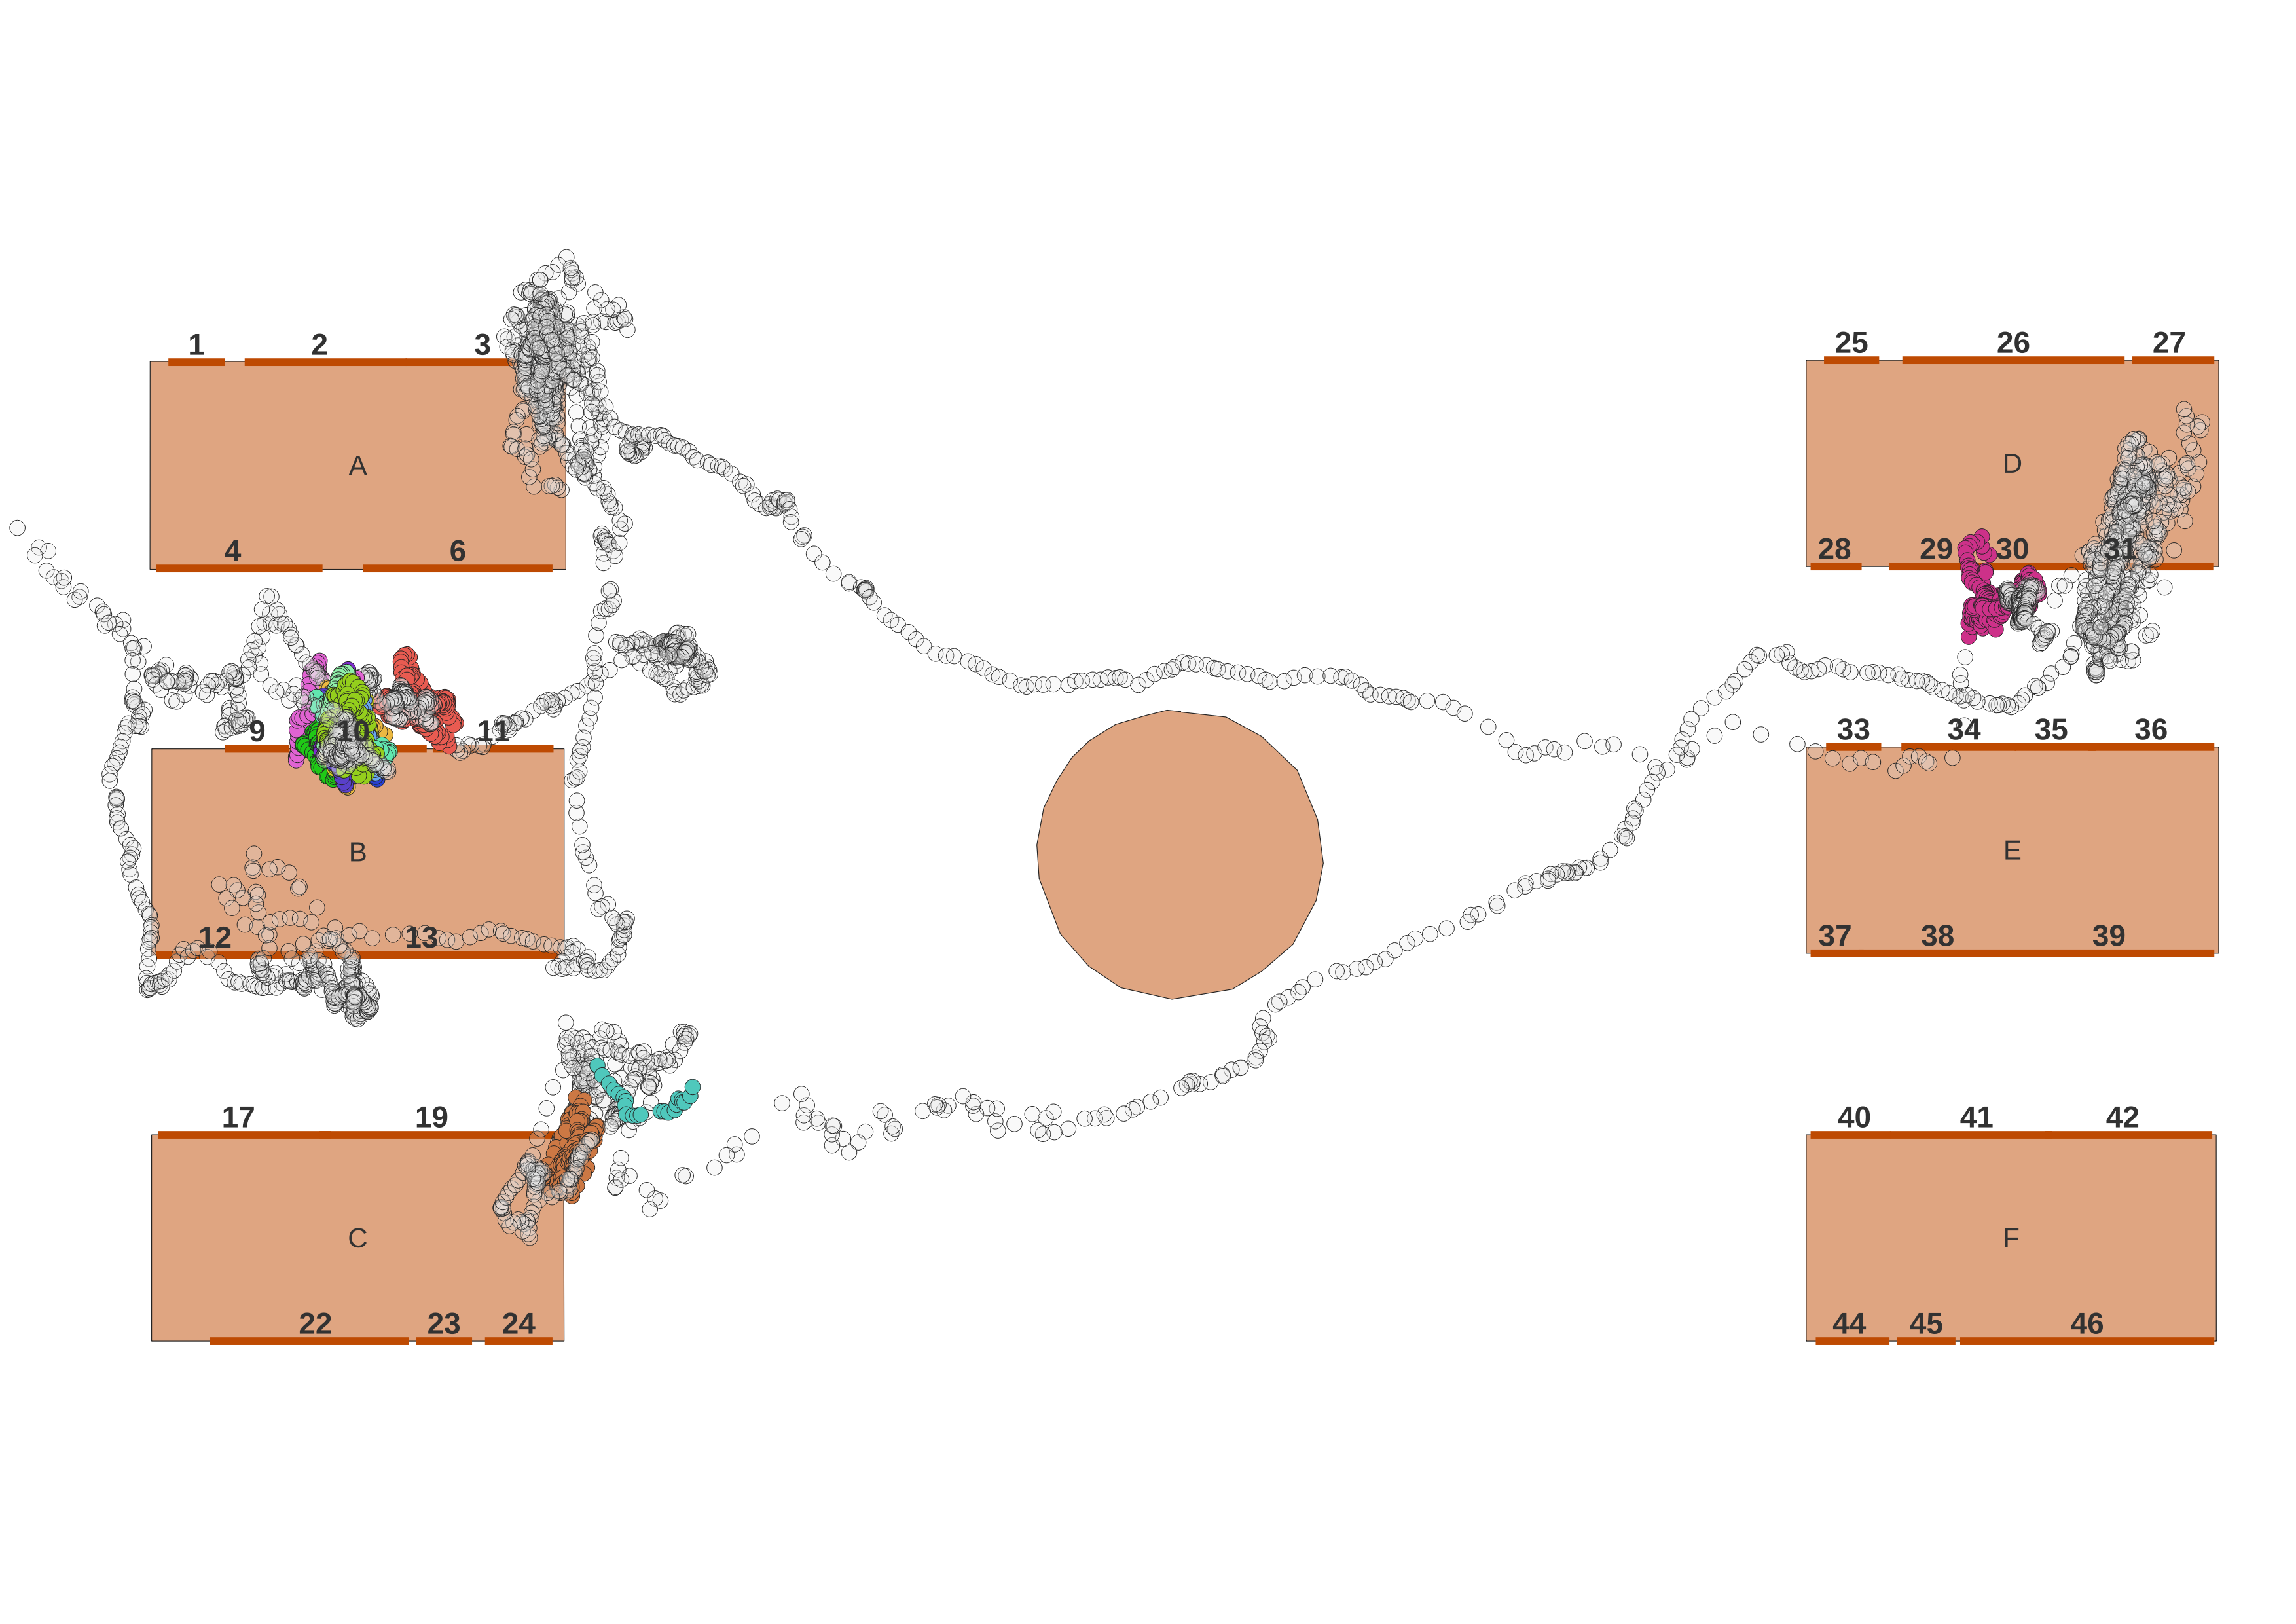
\includegraphics[width=\textwidth]{images/stop_points_p67_PMLH_r1_s20.png}
        \caption{Parametri: $\Delta l_{roam}$=1, $\Delta t_{dur}$=20. Fermate individuate: 17.}
        \label{stop_points_p67_PMLH_r1_s20}
    \end{subfigure}
    \hfill
    \begin{subfigure}[b]{0.45\textwidth}
        \centering
        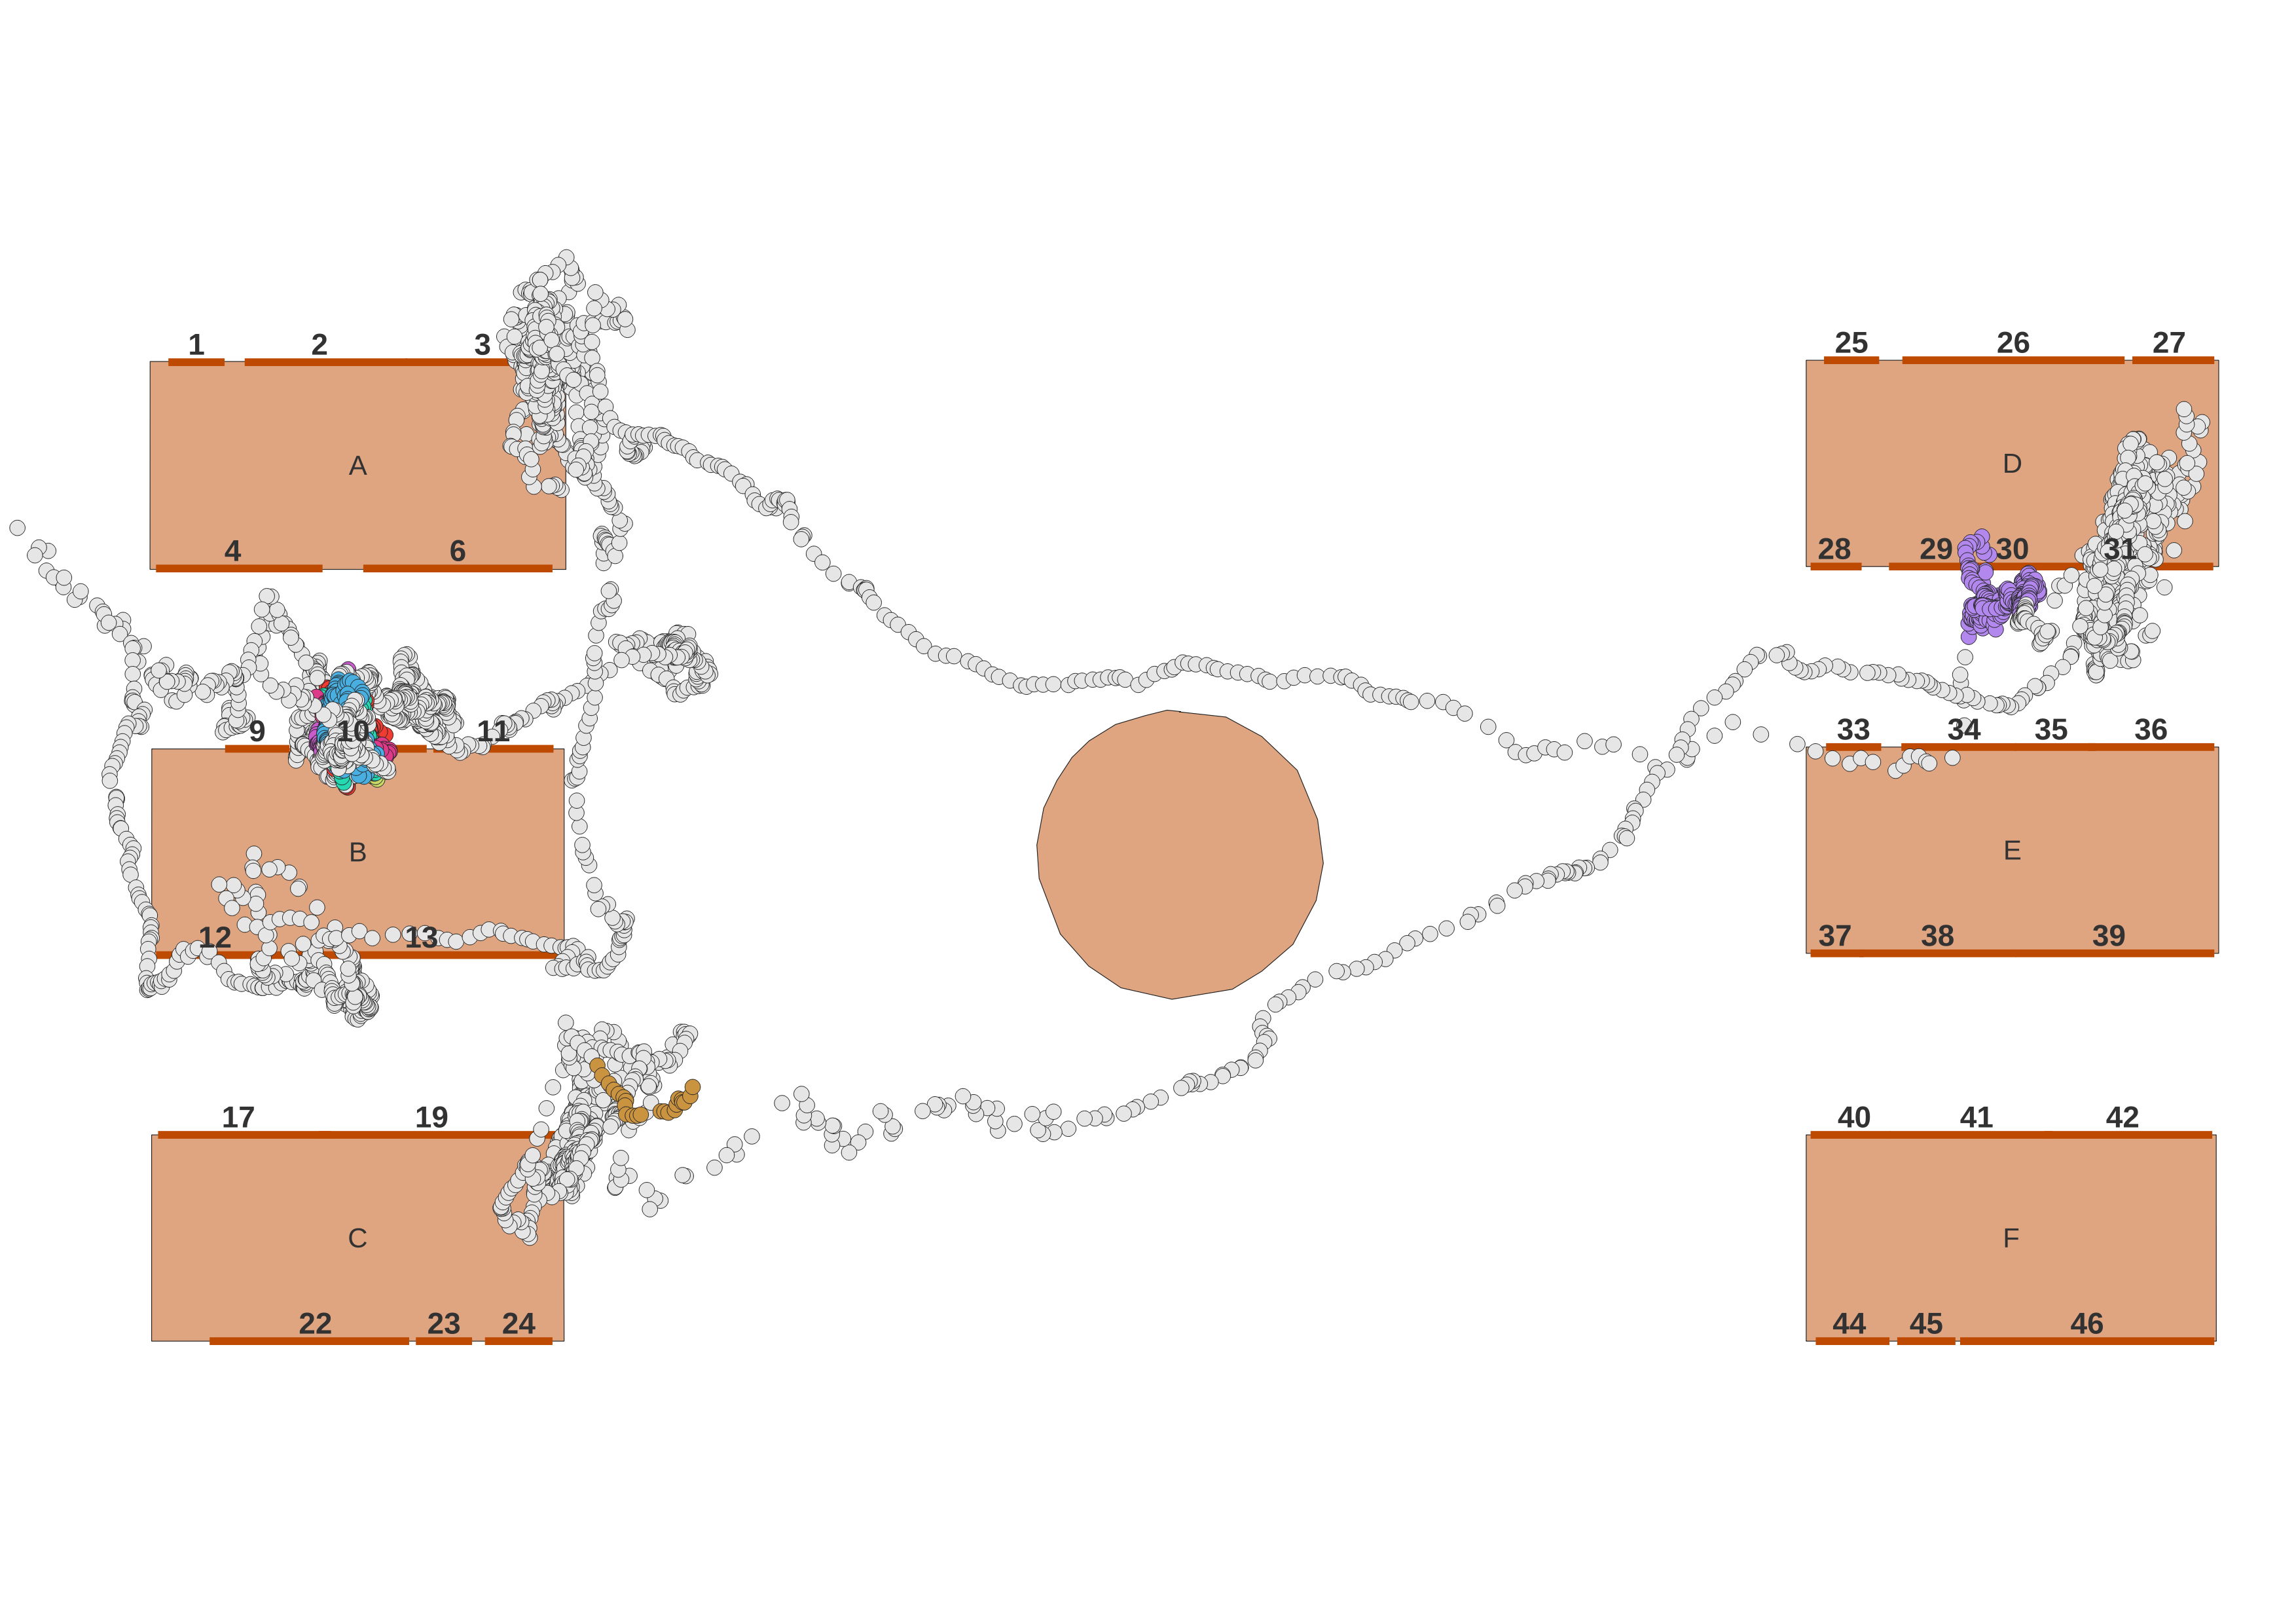
\includegraphics[width=\textwidth]{images/stop_points_p67_PMLH_r1_s30.png}
        \caption{Parametri: $\Delta l_{roam}$=1, $\Delta t_{dur}$=30. Fermate individuate: 8.}
        \label{stop_points_p67_PMLH_r1_s30}
    \end{subfigure}
    \hfill
    \begin{subfigure}[b]{0.45\textwidth}
        \centering
        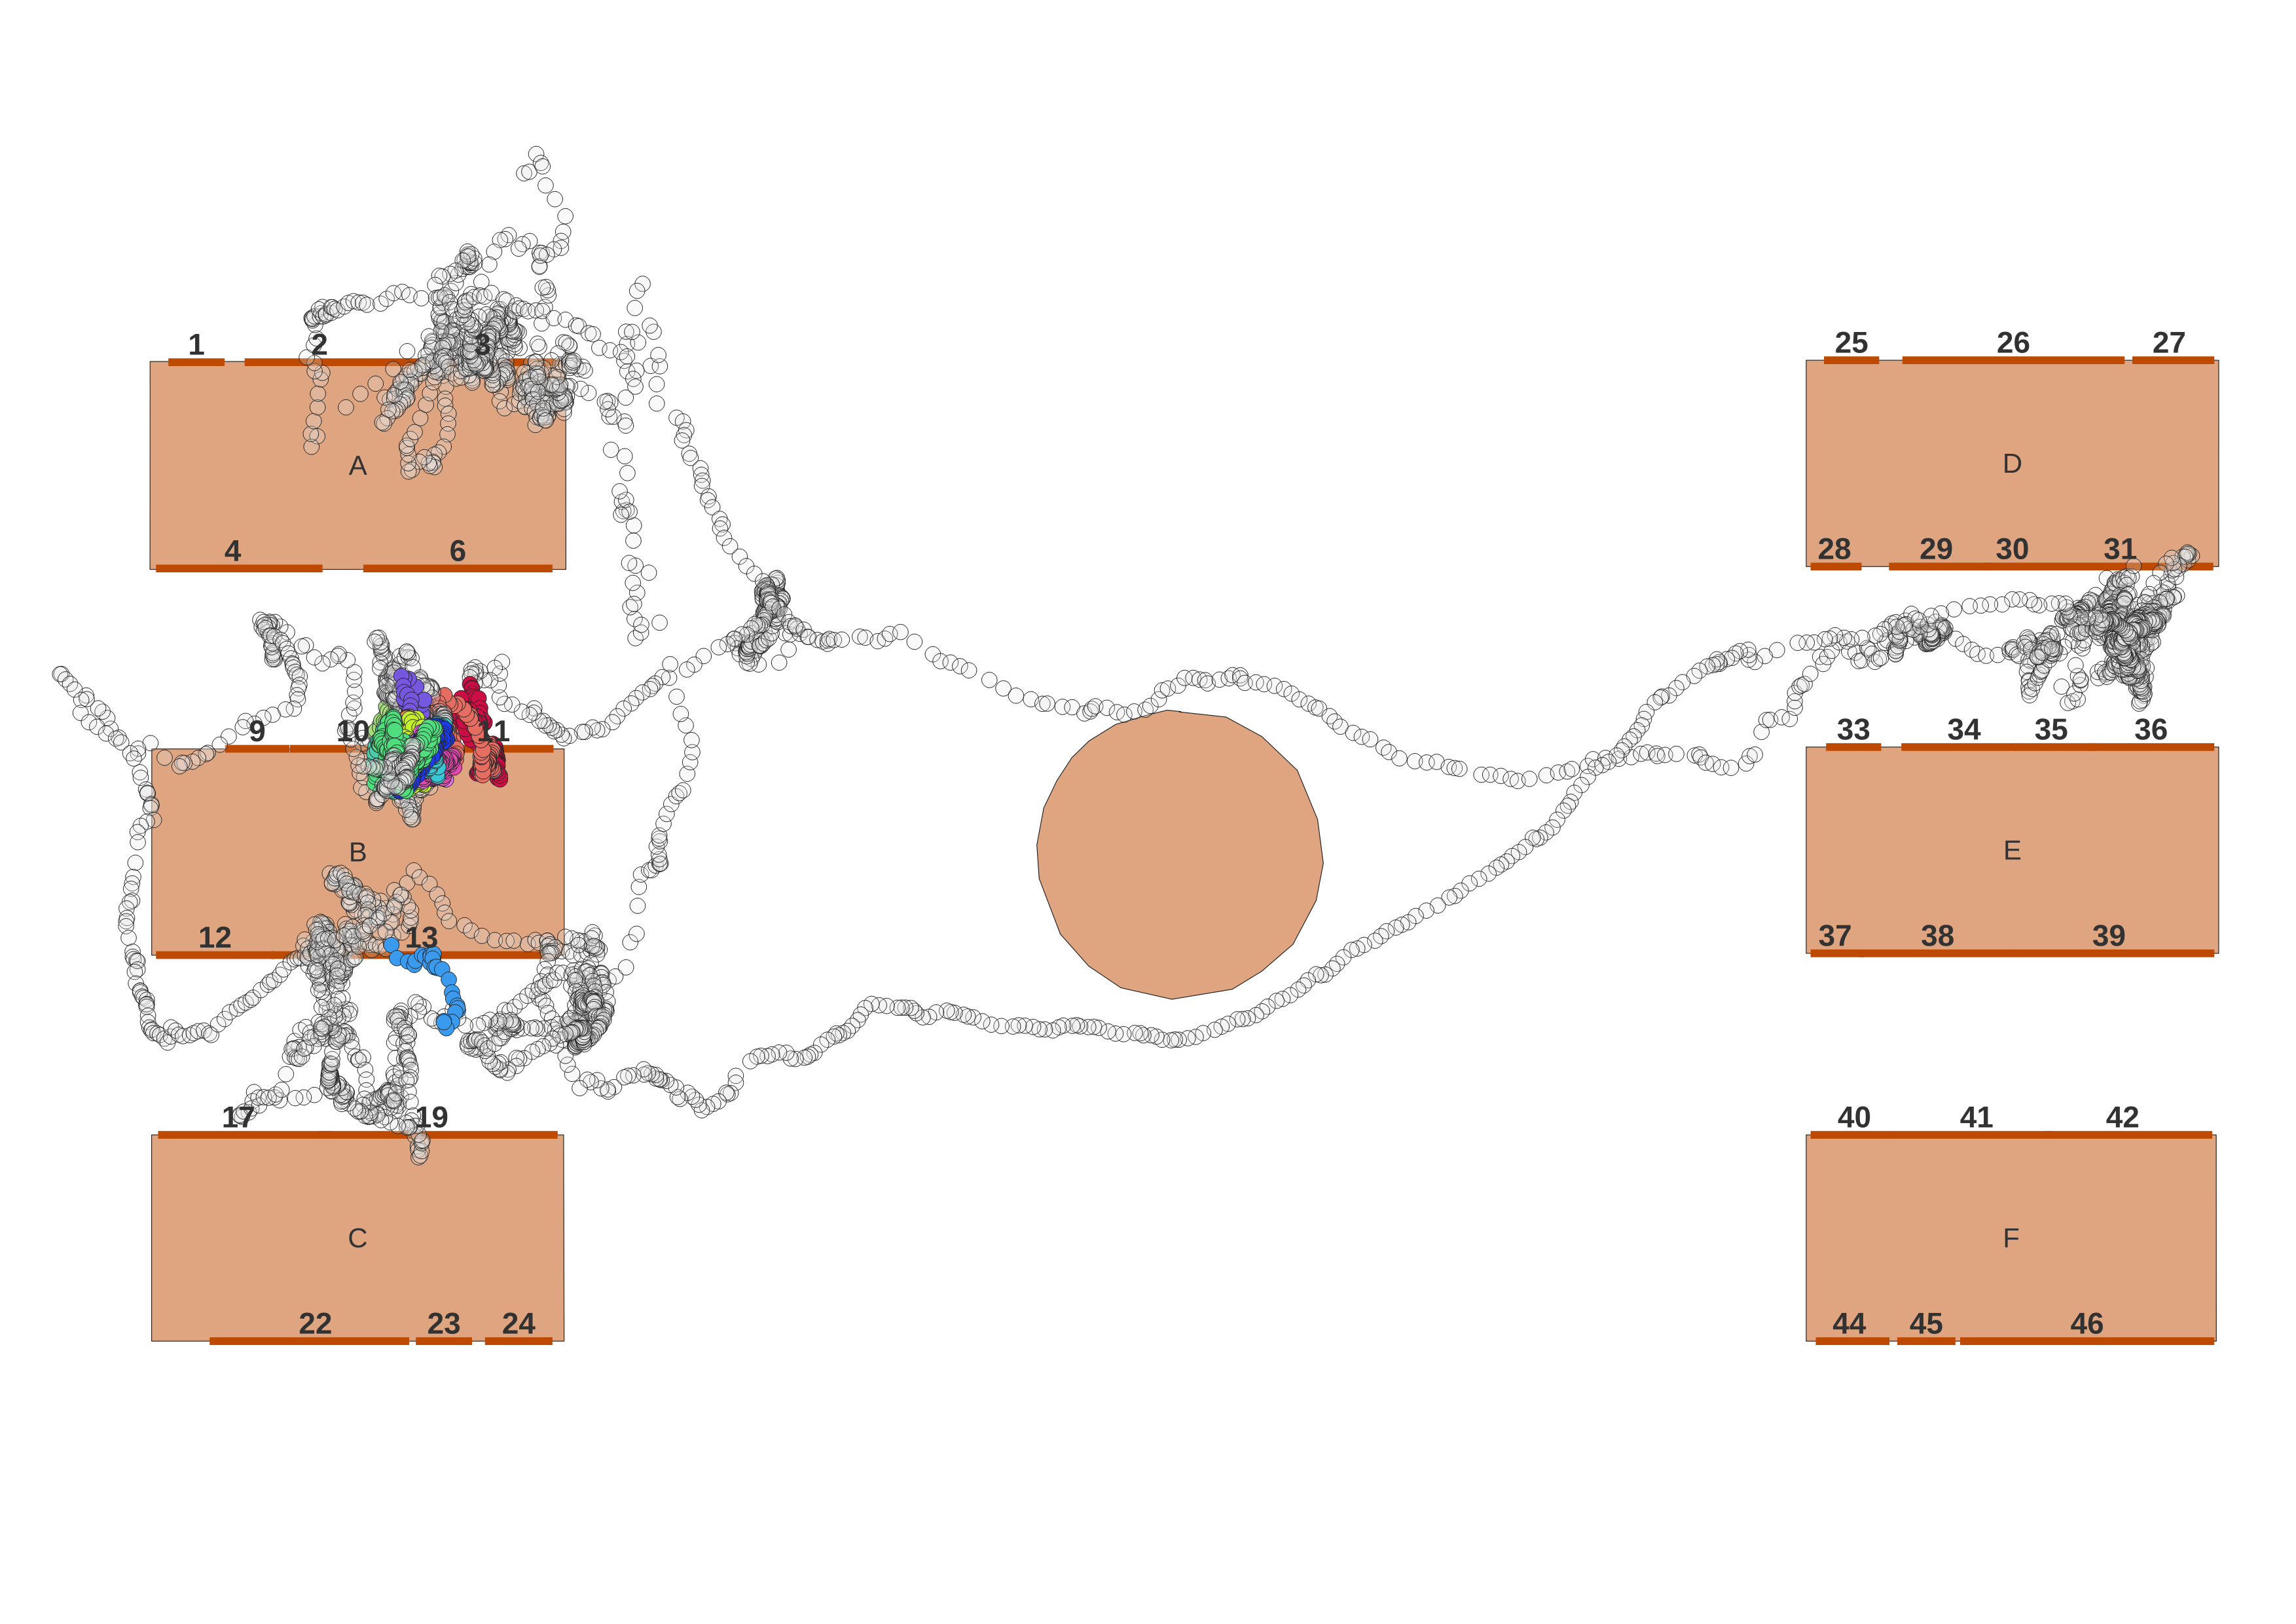
\includegraphics[width=\textwidth]{images/stop_points_p68_PMLH_r1_s20.png}
        \caption{Parametri: $\Delta l_{roam}$=1, $\Delta t_{dur}$=20. Fermate individuate: 14.}
        \label{stop_points_p68_PMLH_r1_s20}
    \end{subfigure}
    \hfill
    \begin{subfigure}[b]{0.45\textwidth}
        \centering
        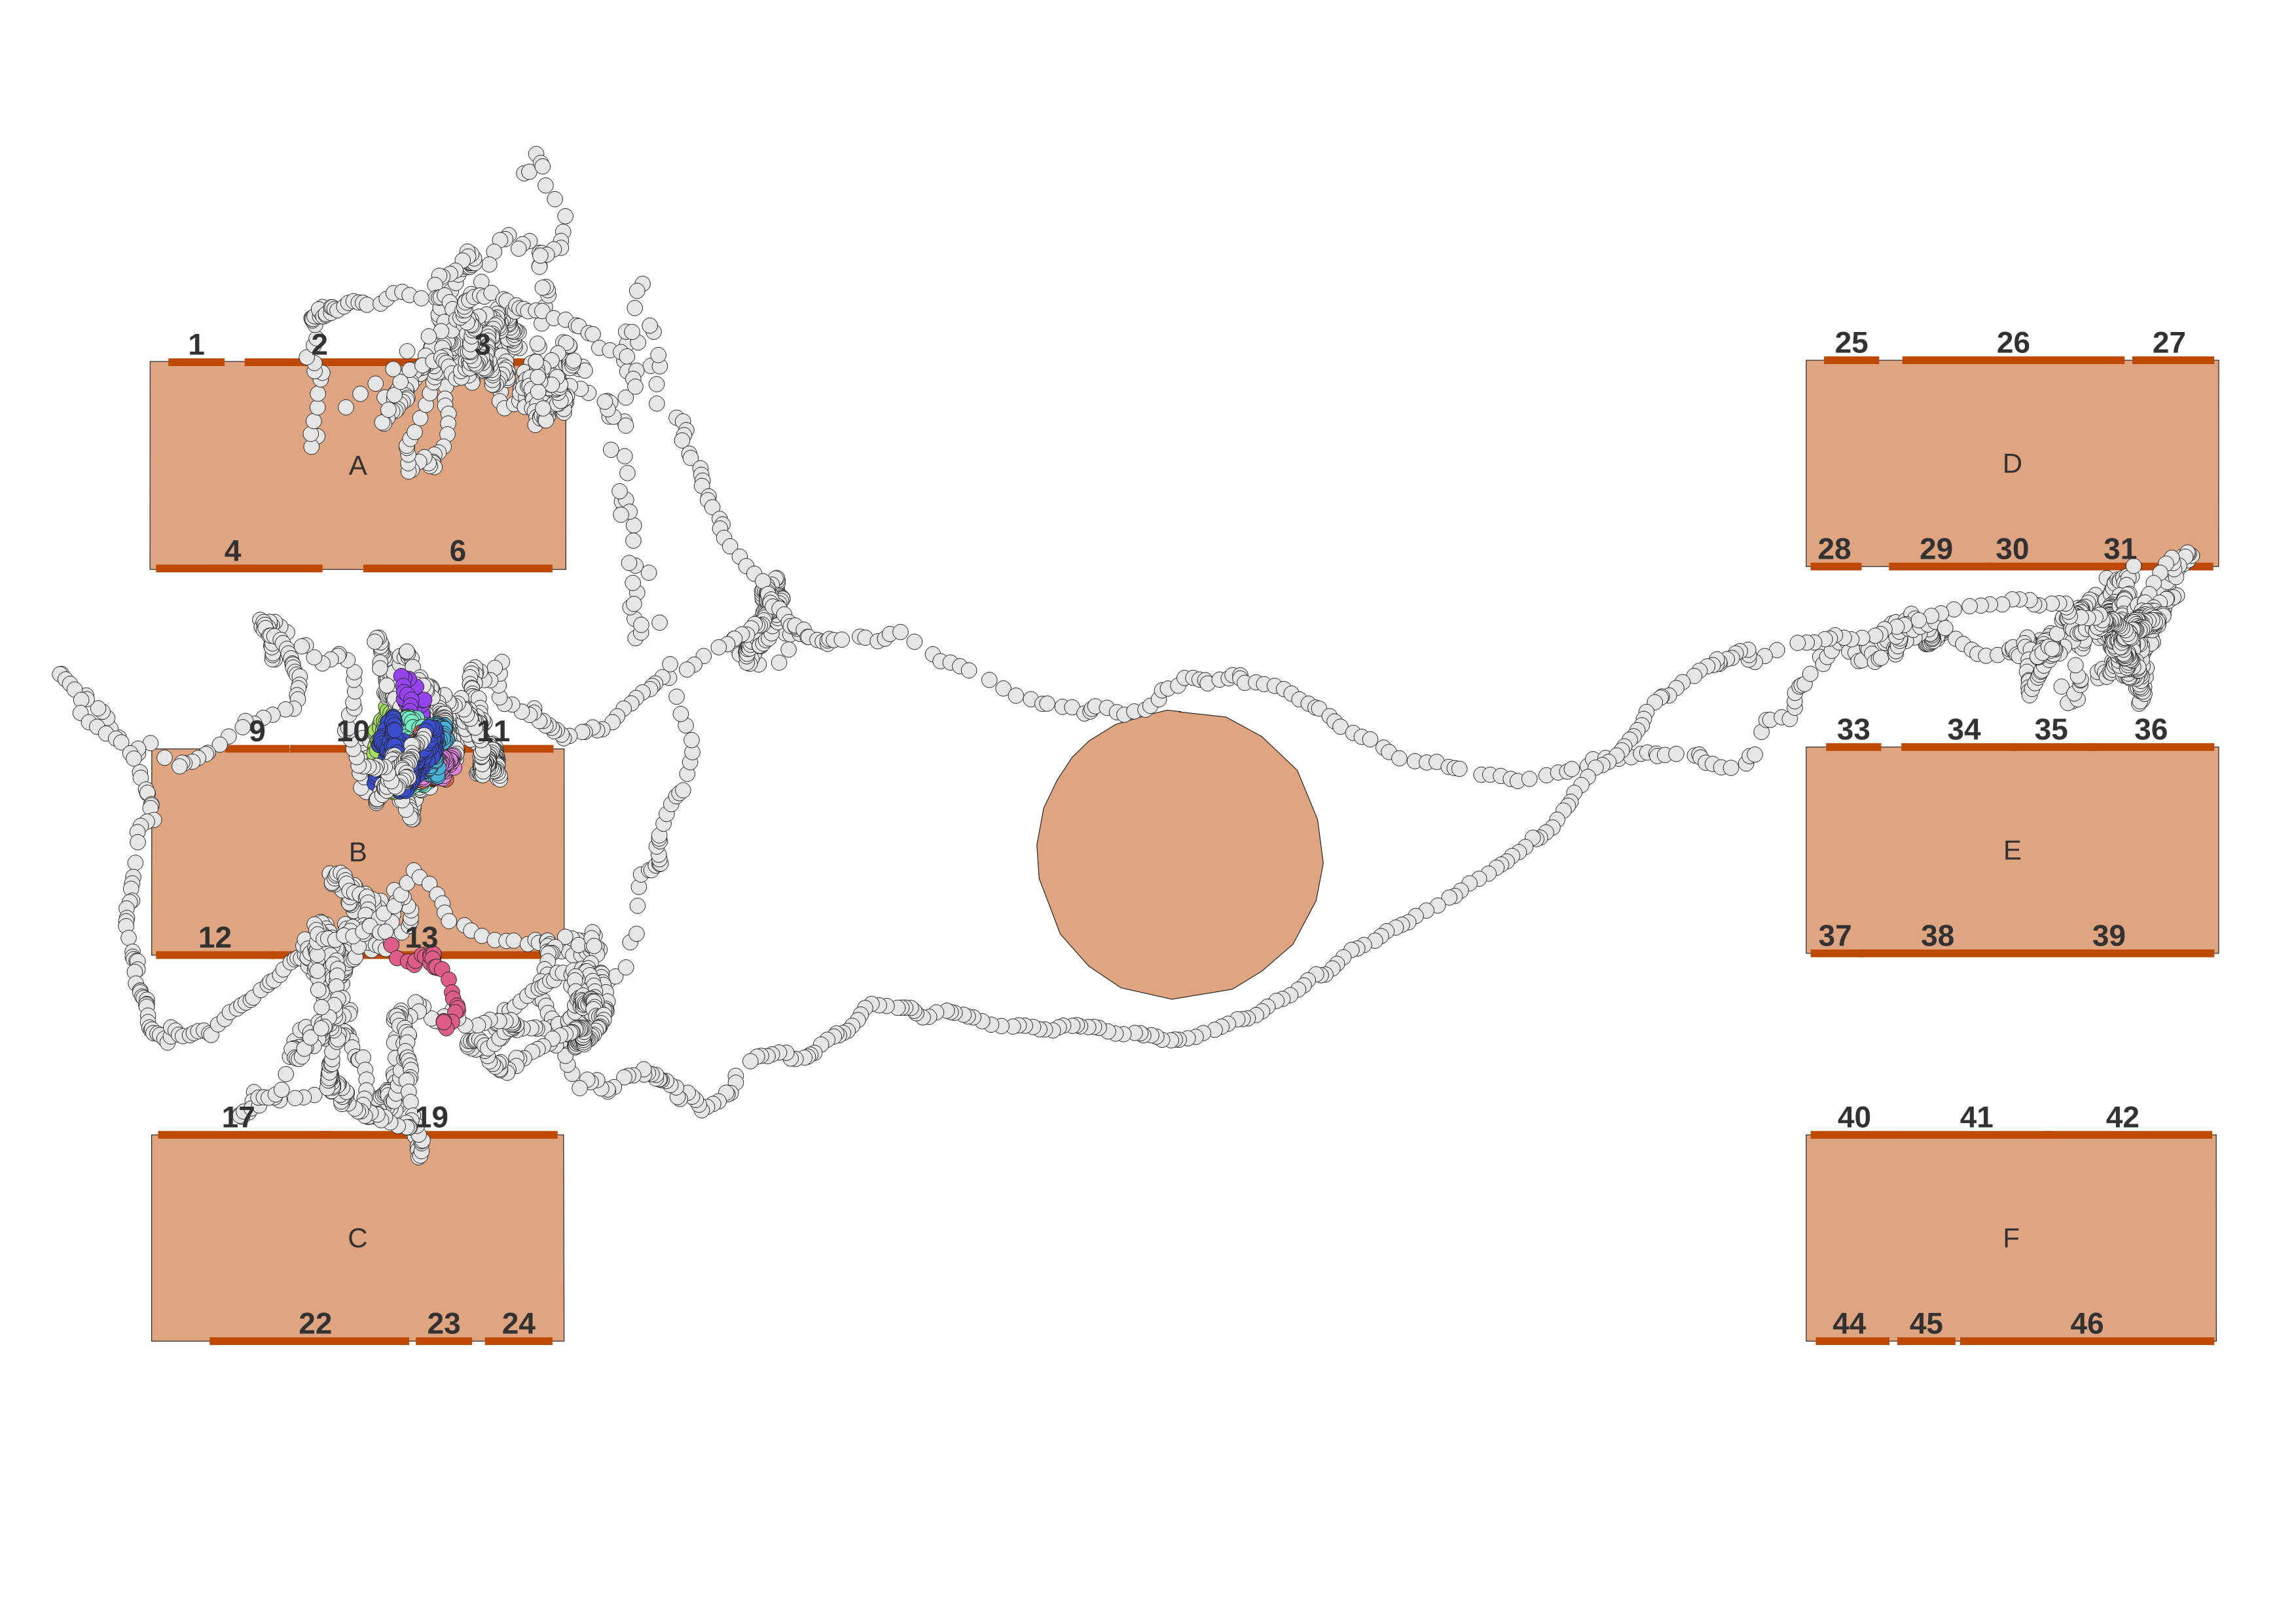
\includegraphics[width=\textwidth]{images/stop_points_p68_PMLH_r1_s30.png}
        \caption{Parametri: $\Delta l_{roam}$=1, $\Delta t_{dur}$=30. Fermate individuate: 8.}
        \label{stop_points_p68_PMLH_r1_s30}
    \end{subfigure}
    \hfill
    \caption{Punti di stop della persona 57 (a,b), della persona 67 (c,d) e della persona 68 (e,f), individuati con l'algoritmo PMLH.}
    \label{stop_points_PMLH}
\end{figure}

\begin{figure}[htb!]
    \centering
    \begin{subfigure}[b]{0.45\textwidth}
        \centering
        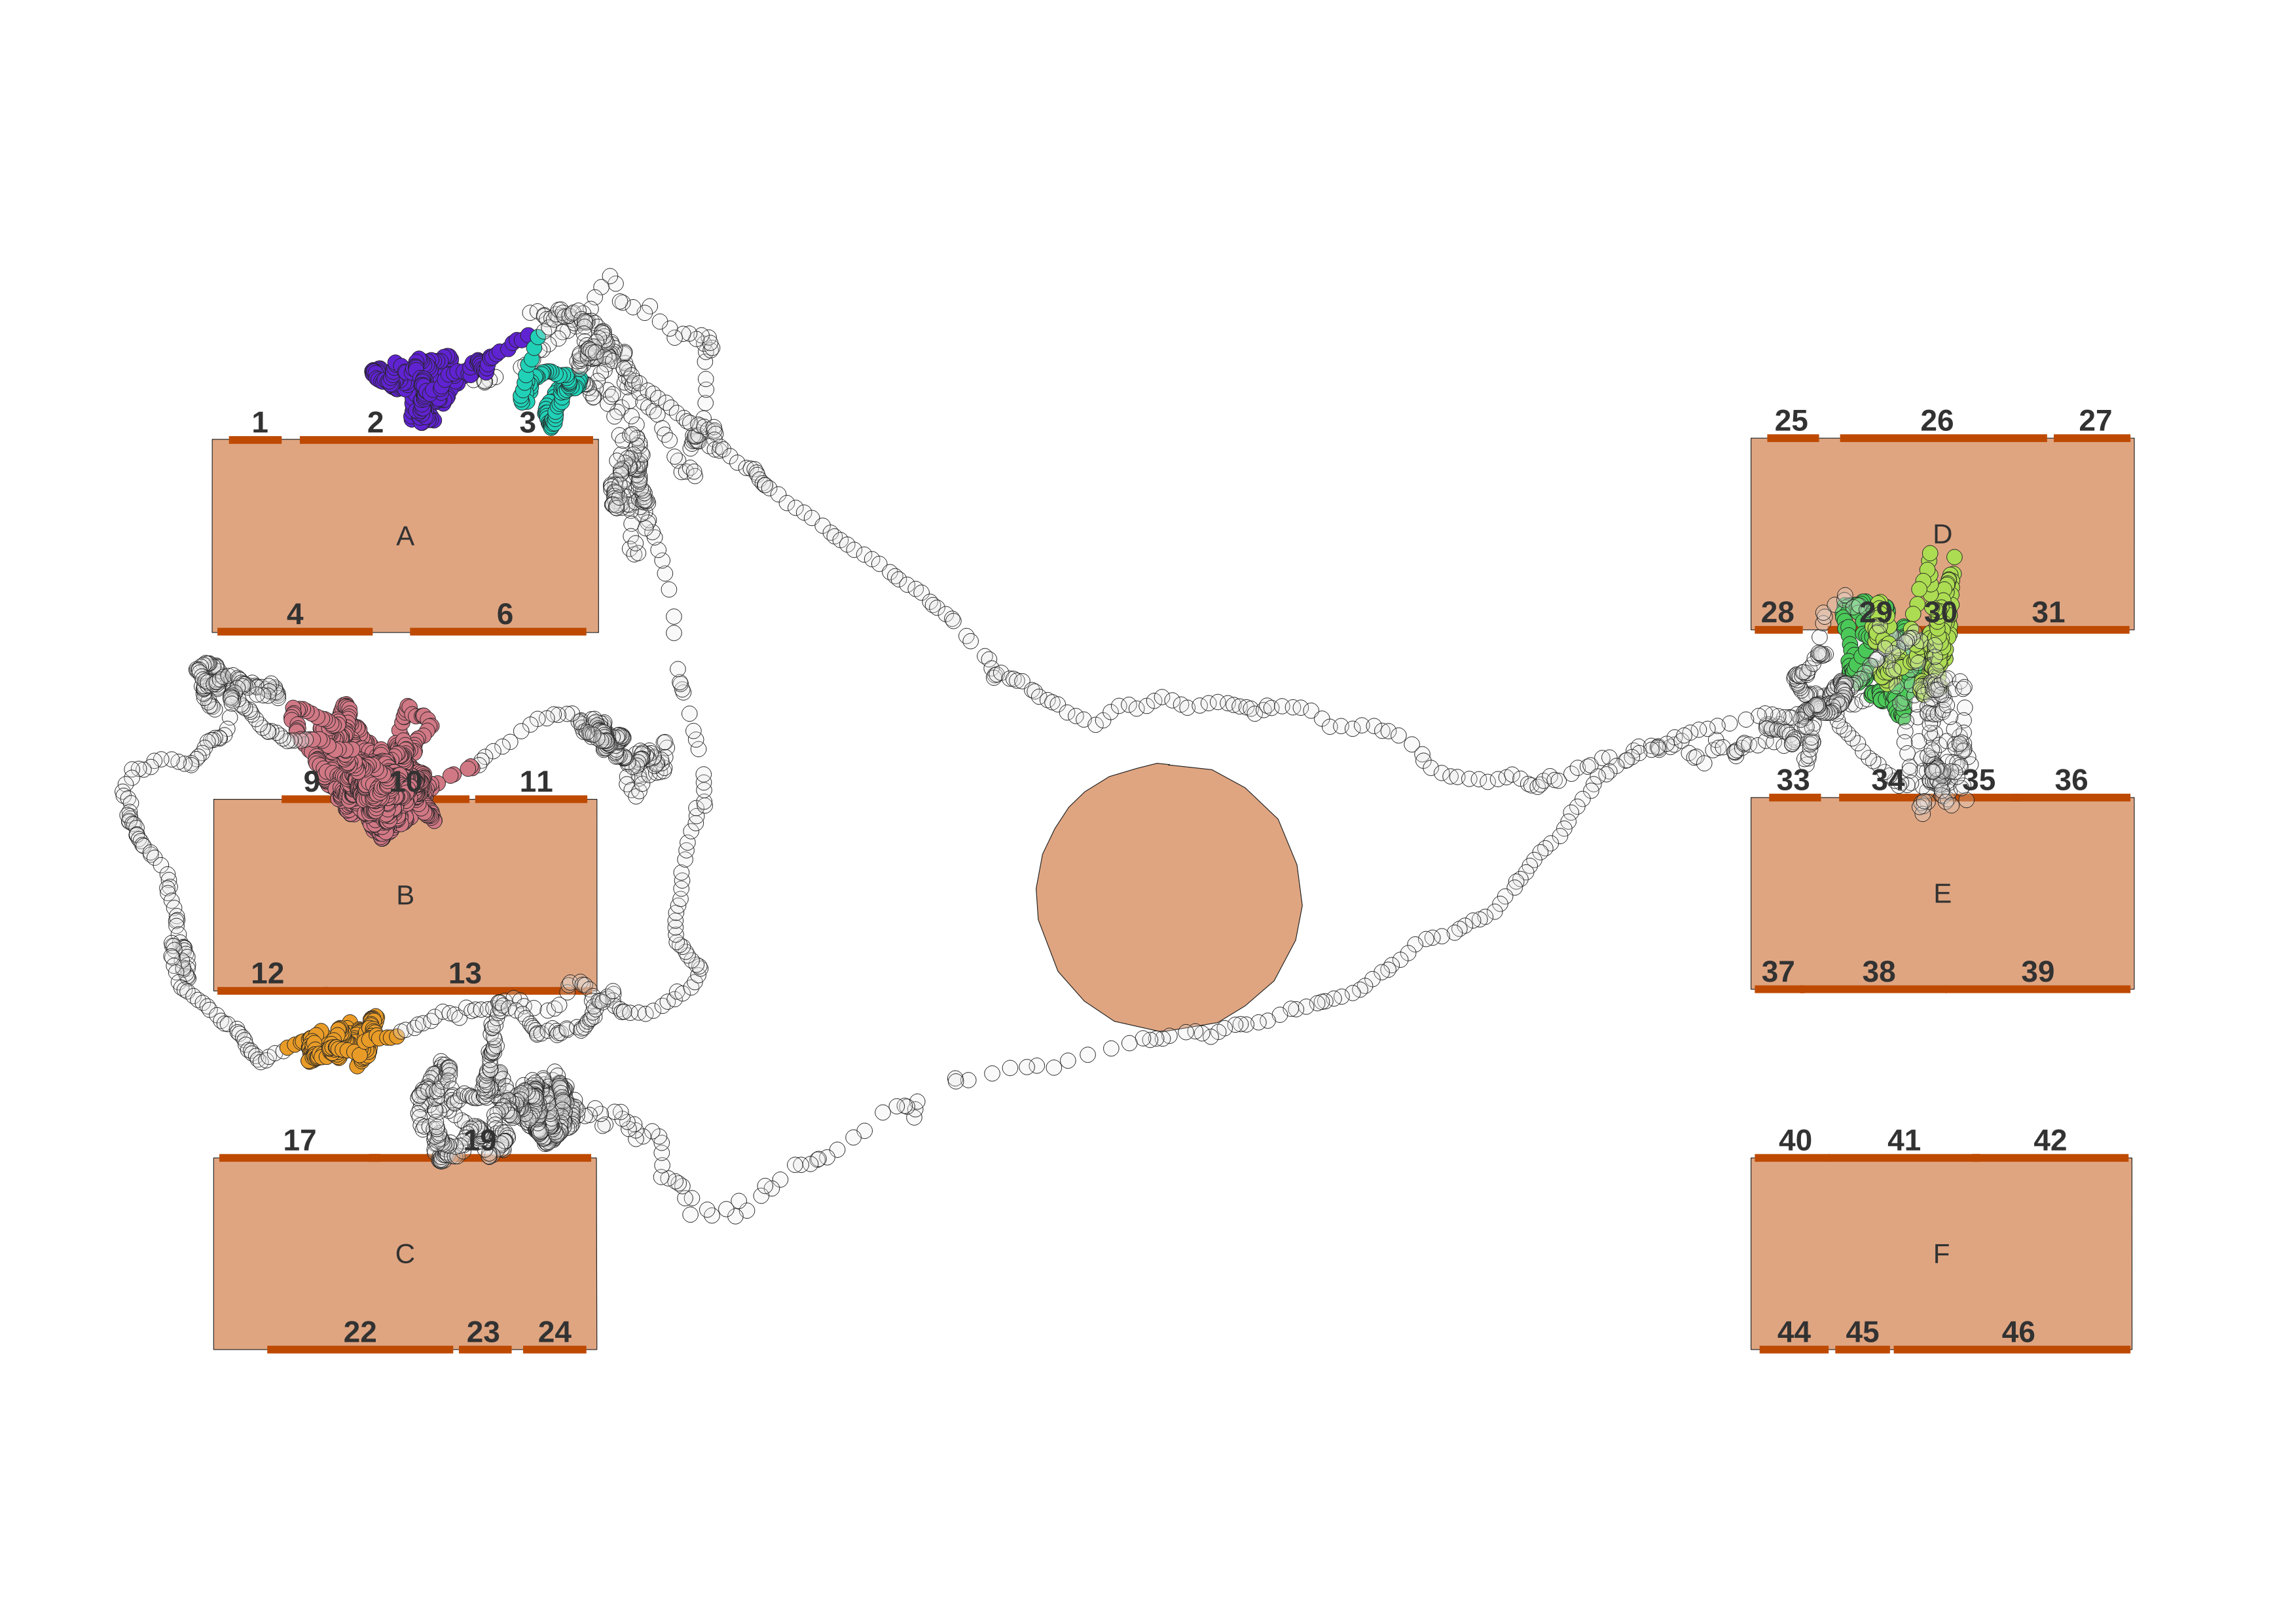
\includegraphics[width=\textwidth]{images/stop_points_p57_SOC_eps1_tau20_minMov05.png}
        \caption{Parametri: eps=1, tau=20, minMov=0.5. Fermate individuate: 6.}
        \label{stop_points_p57_SOC_eps1_tau20_minMov05}
    \end{subfigure}
    \hfill
    \begin{subfigure}[b]{0.45\textwidth}
        \centering
        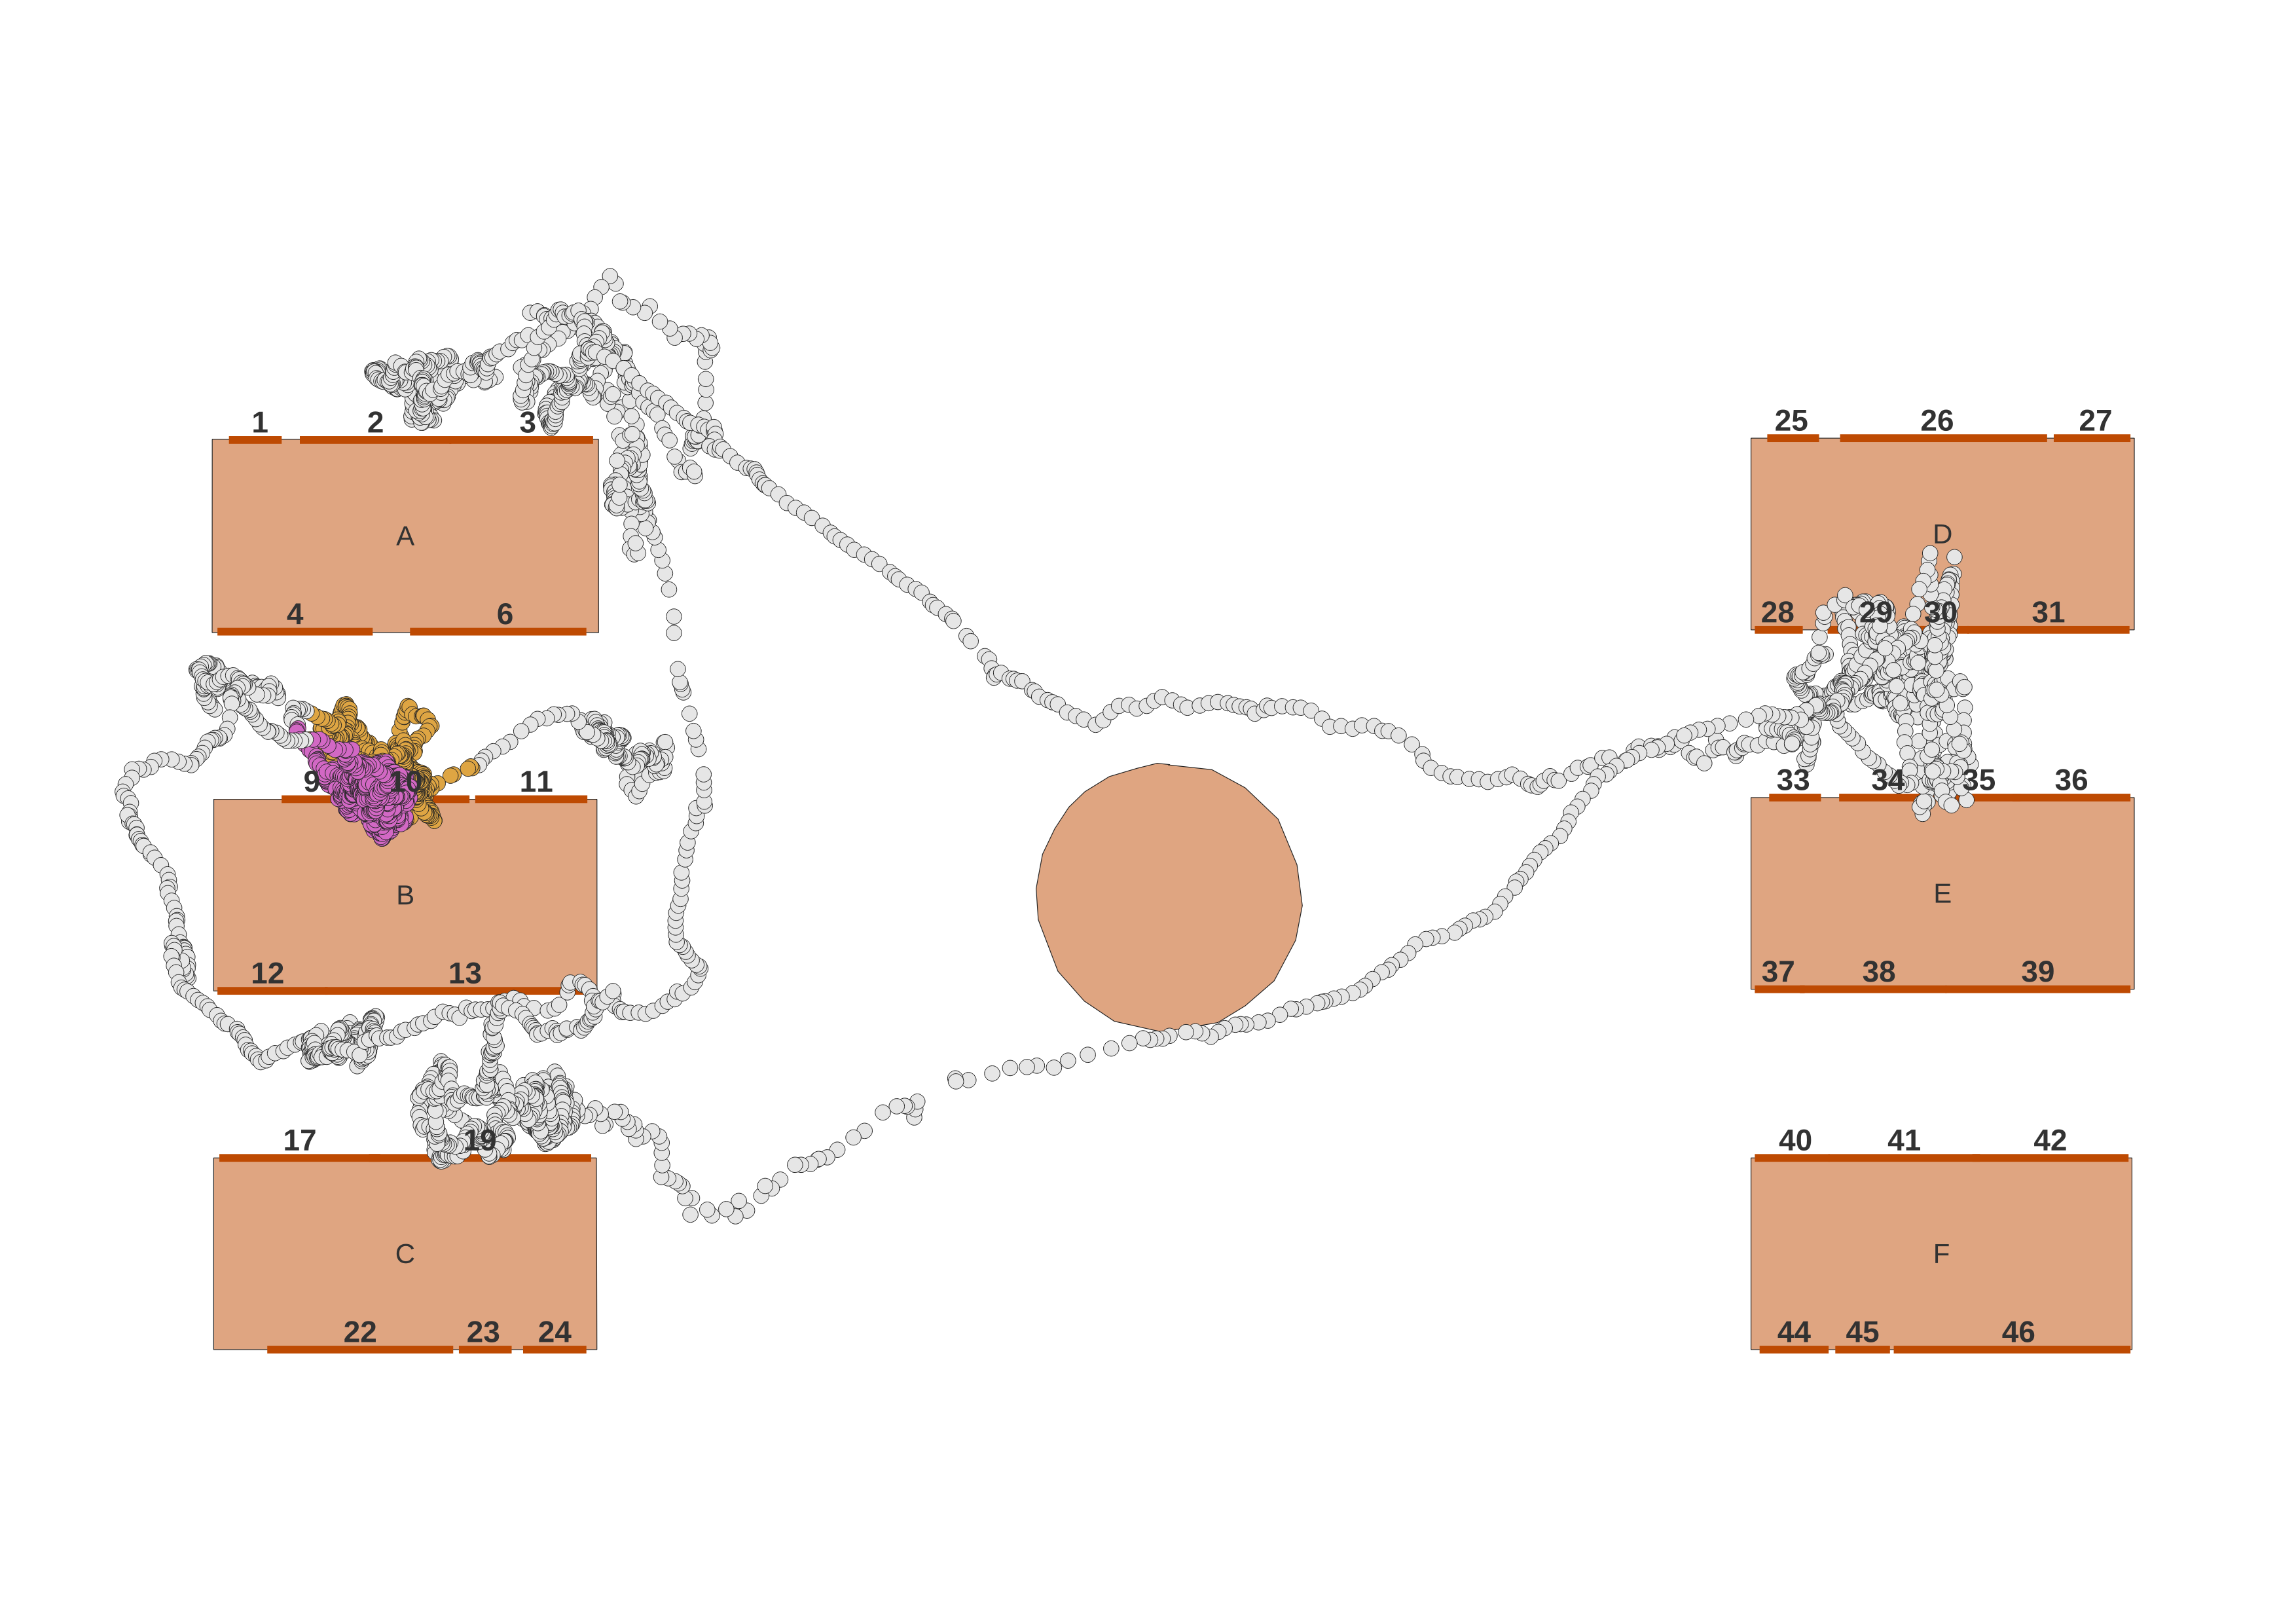
\includegraphics[width=\textwidth]{images/stop_points_p57_SOC_eps1_tau30_minMov05.png}
        \caption{Parametri: eps=1, tau=30, minMov=0.5. Fermate individuate: 2.}
        \label{stop_points_p57_SOC_eps1_tau30_minMov05}
    \end{subfigure}
    \hfill
    \begin{subfigure}[b]{0.45\textwidth}
        \centering
        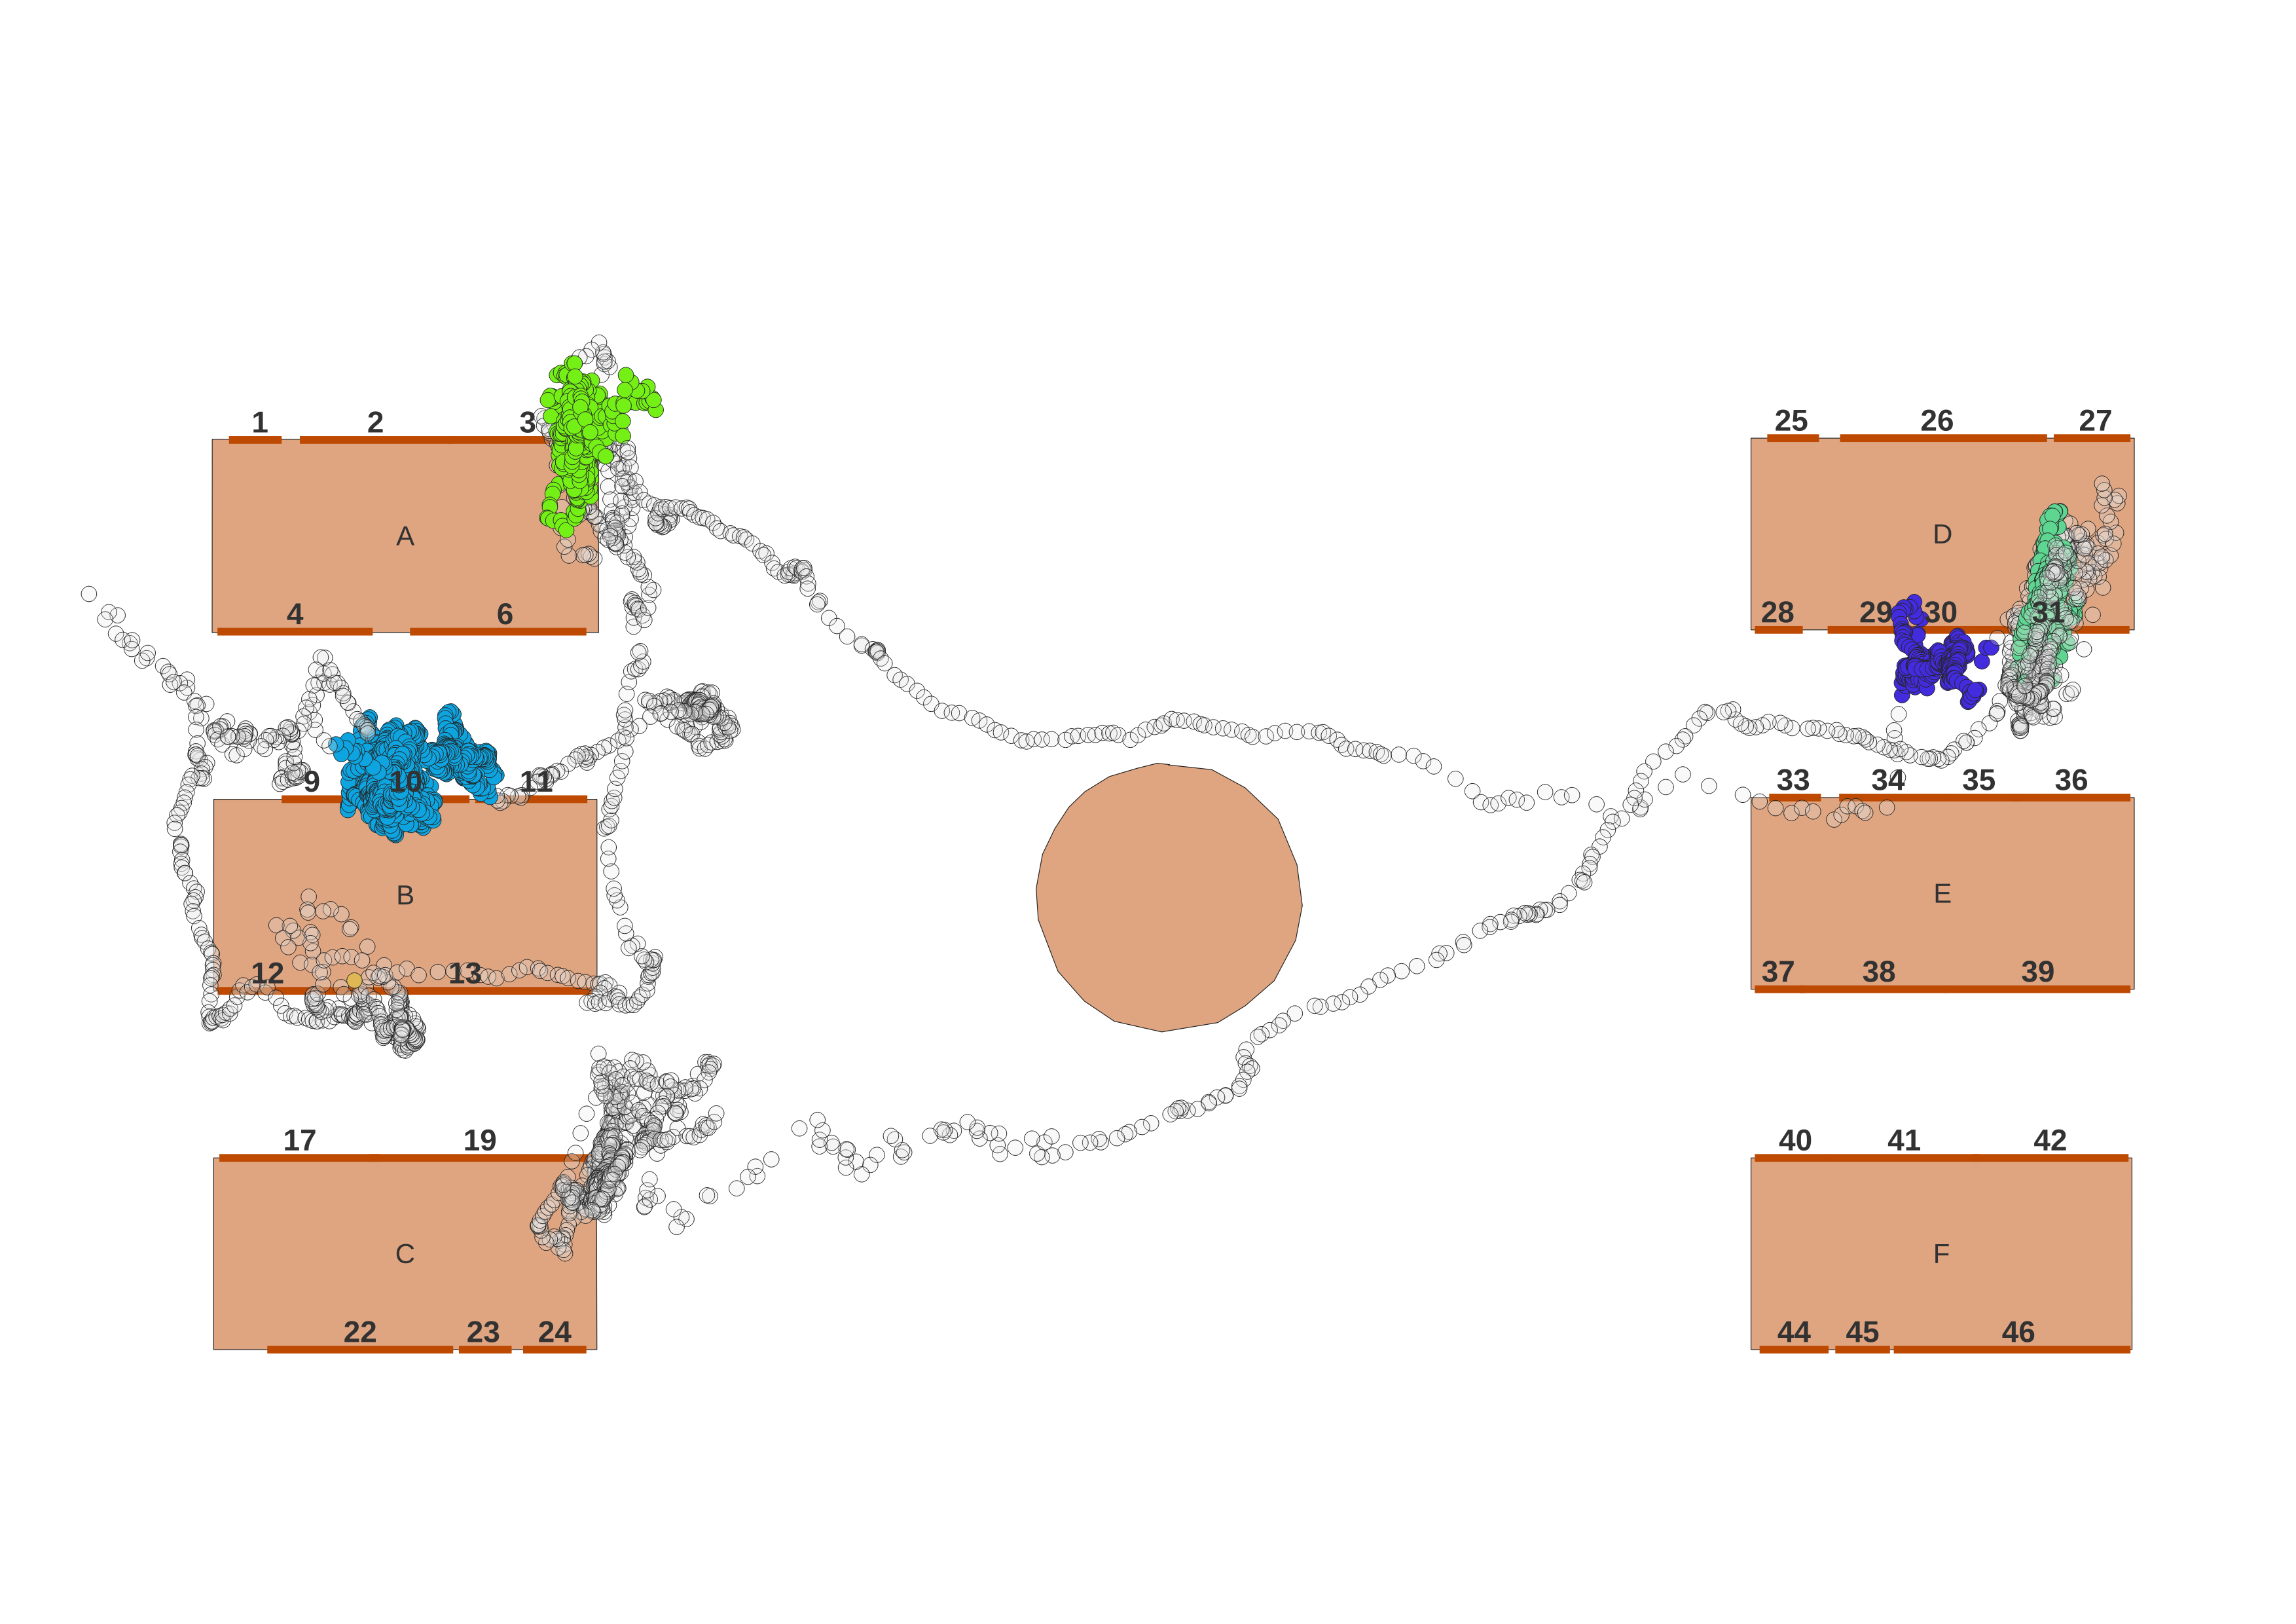
\includegraphics[width=\textwidth]{images/stop_points_p67_SOC_eps1_tau20_minMov05.png}
        \caption{Parametri: eps=1, tau=20, minMov=0.5. Fermate individuate: 5.}
        \label{stop_points_p67_SOC_eps1_tau20_minMov05}
    \end{subfigure}
    \hfill
    \begin{subfigure}[b]{0.45\textwidth}
        \centering
        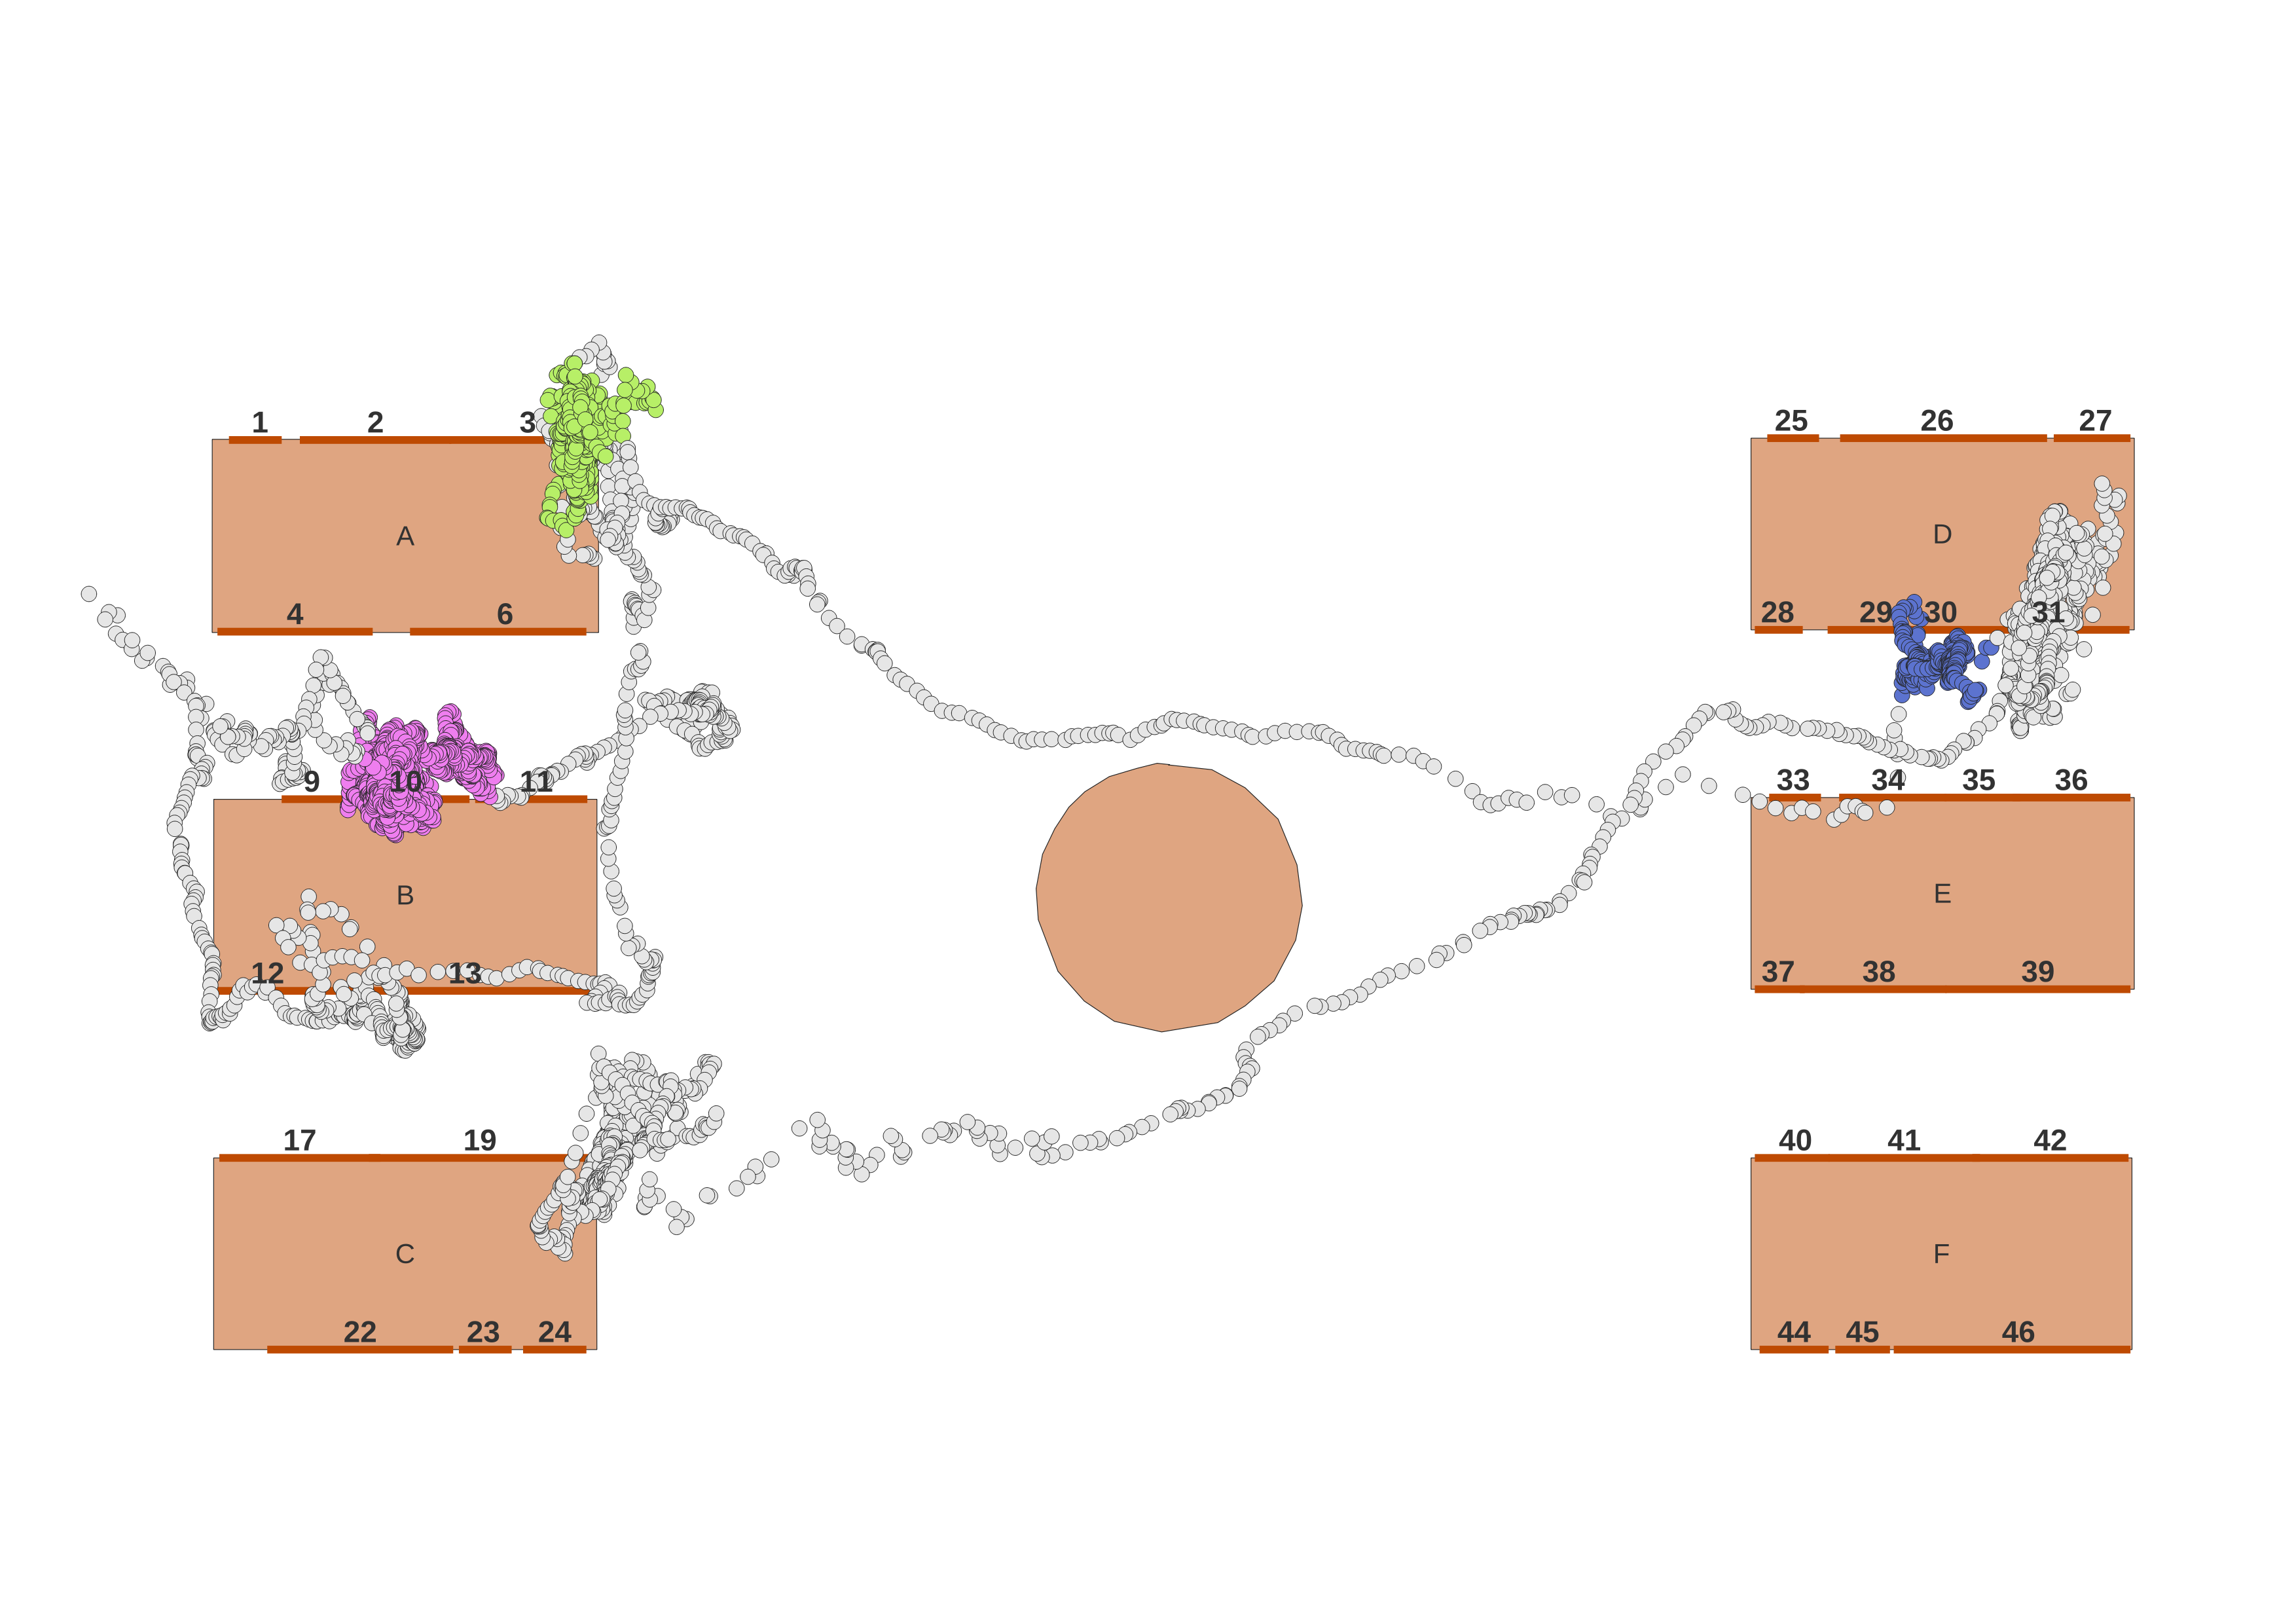
\includegraphics[width=\textwidth]{images/stop_points_p67_SOC_eps1_tau30_minMov05.png}
        \caption{Parametri: eps=1, tau=30, minMov=0.5. Fermate individuate: 3.}
        \label{stop_points_p67_SOC_eps1_tau30_minMov05}
    \end{subfigure}
    \hfill
    \begin{subfigure}[b]{0.45\textwidth}
        \centering
        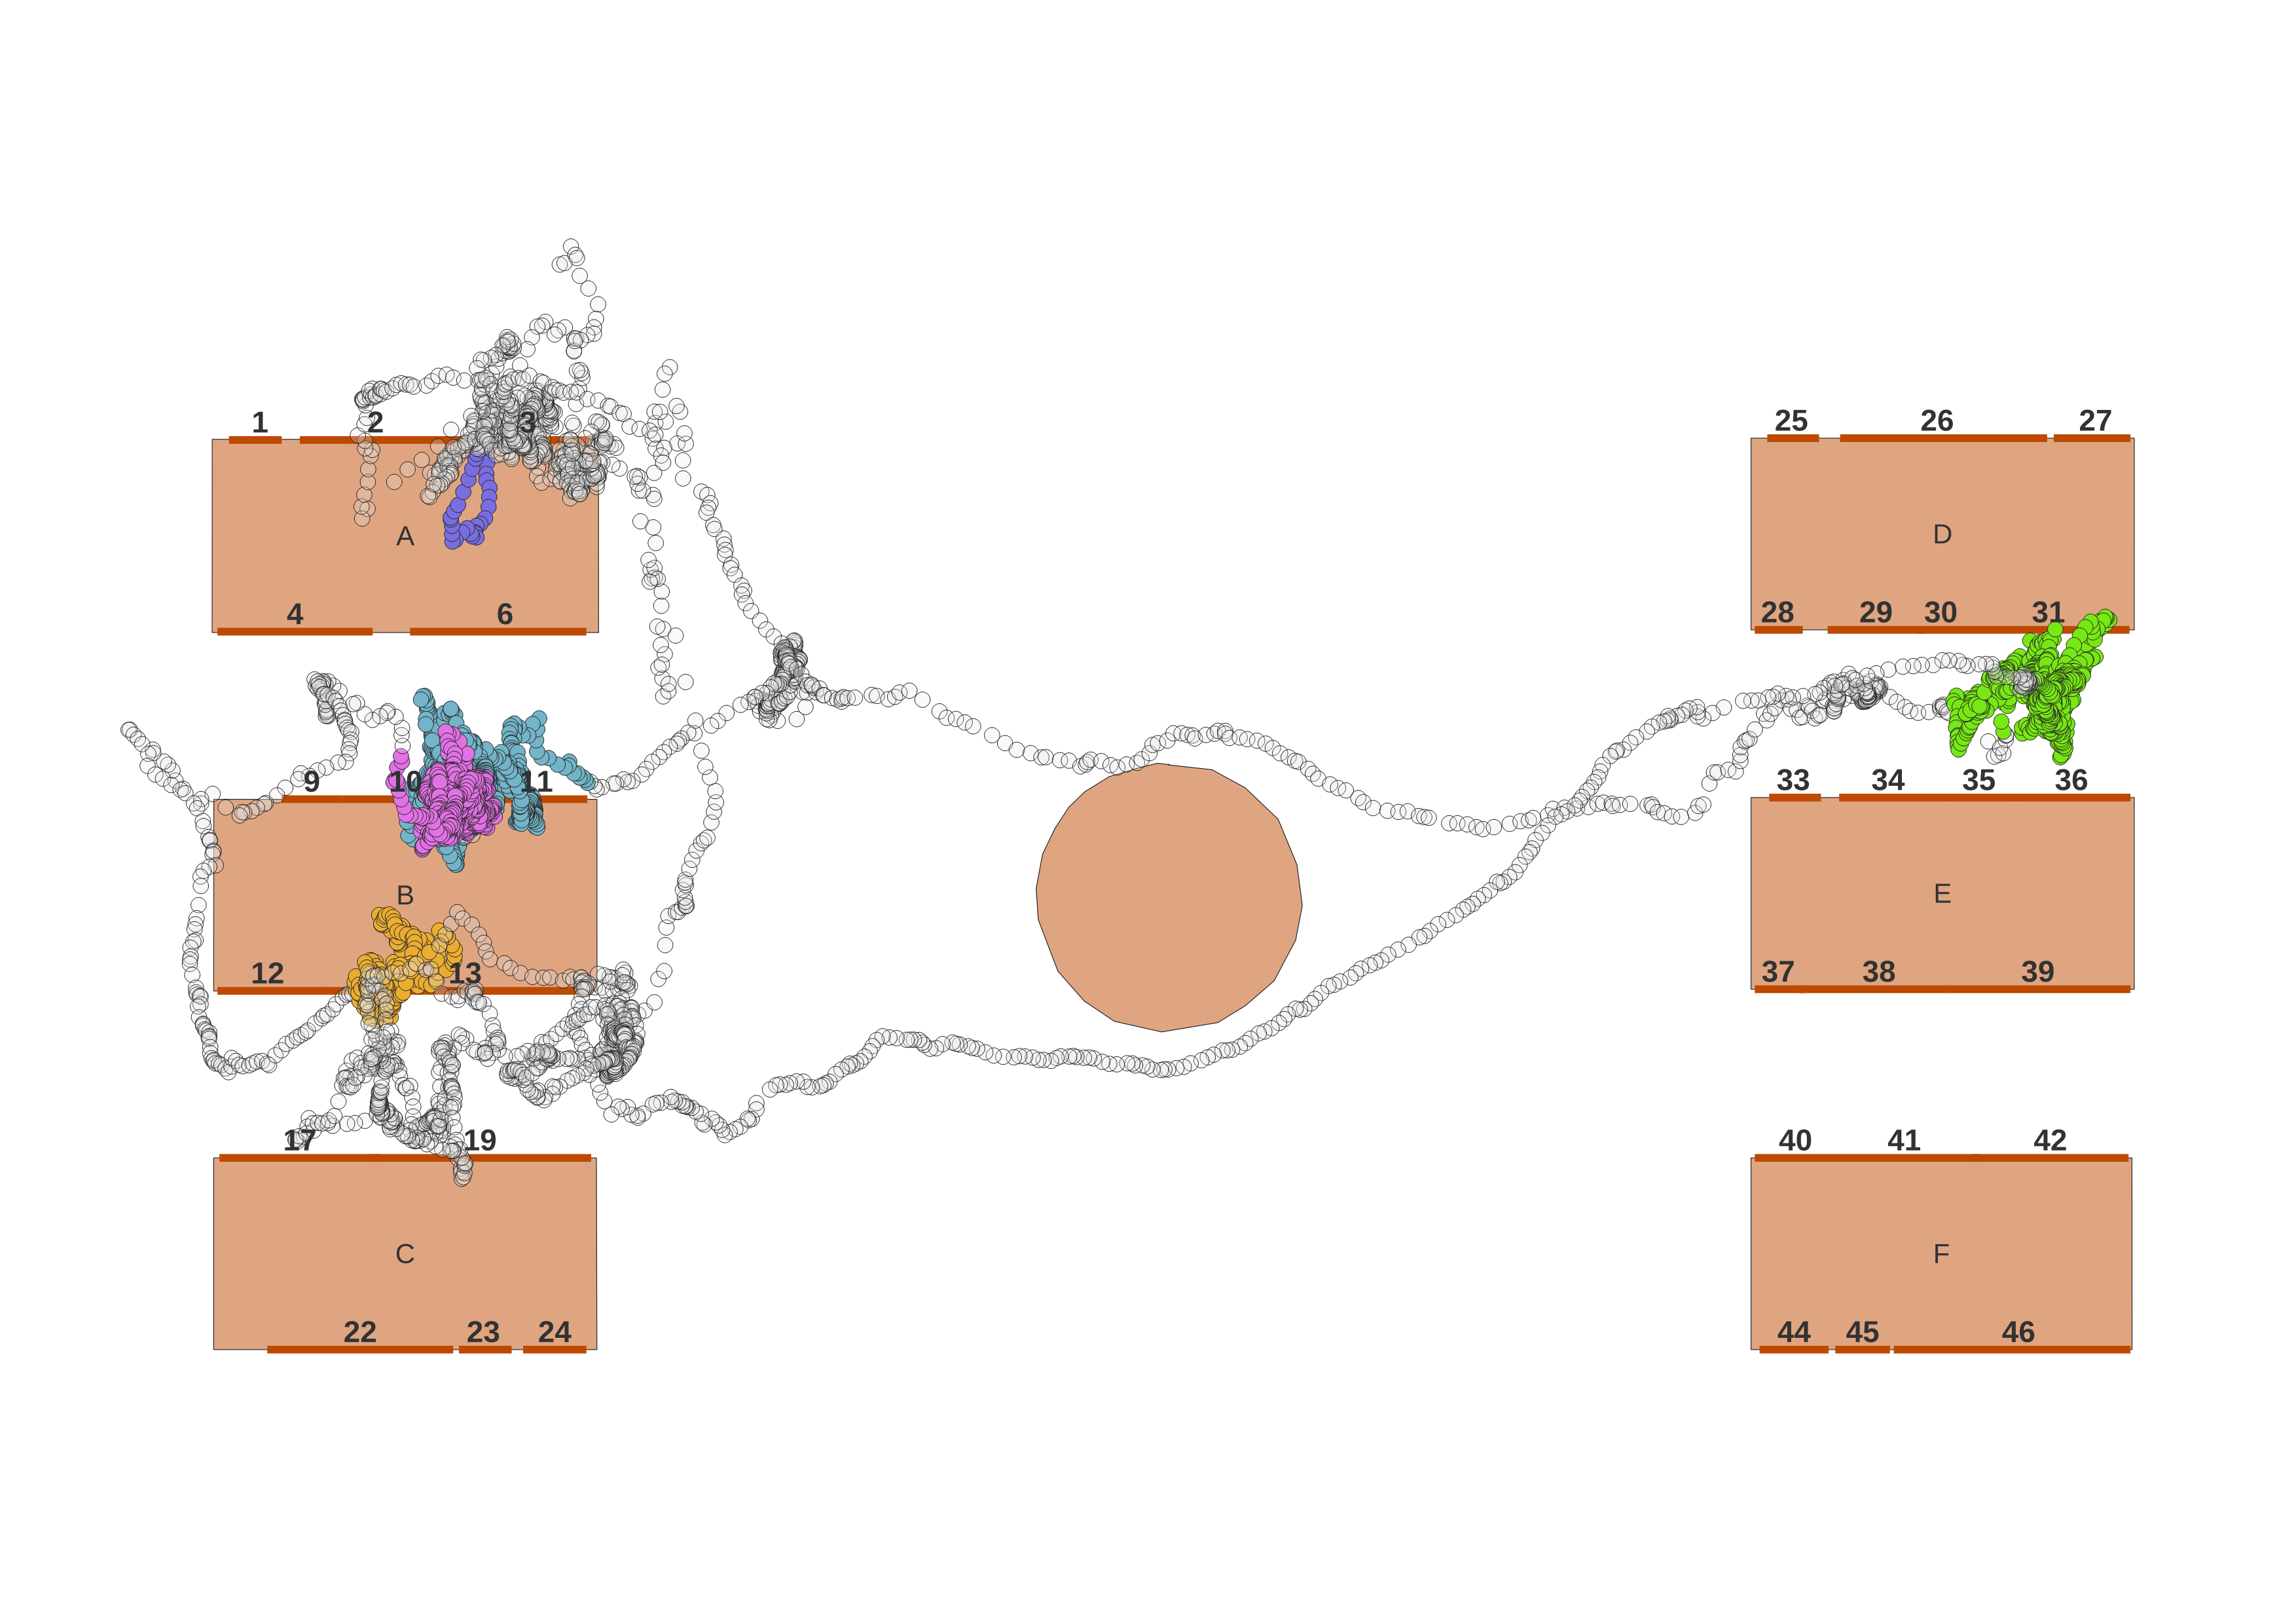
\includegraphics[width=\textwidth]{images/stop_points_p68_SOC_eps1_tau20_minMov05.png}
        \caption{Parametri: eps=1, tau=20, minMov=0.5. Fermate individuate: 5.}
        \label{stop_points_p68_SOC_eps1_tau20_minMov05}
    \end{subfigure}
    \hfill
    \begin{subfigure}[b]{0.45\textwidth}
        \centering
        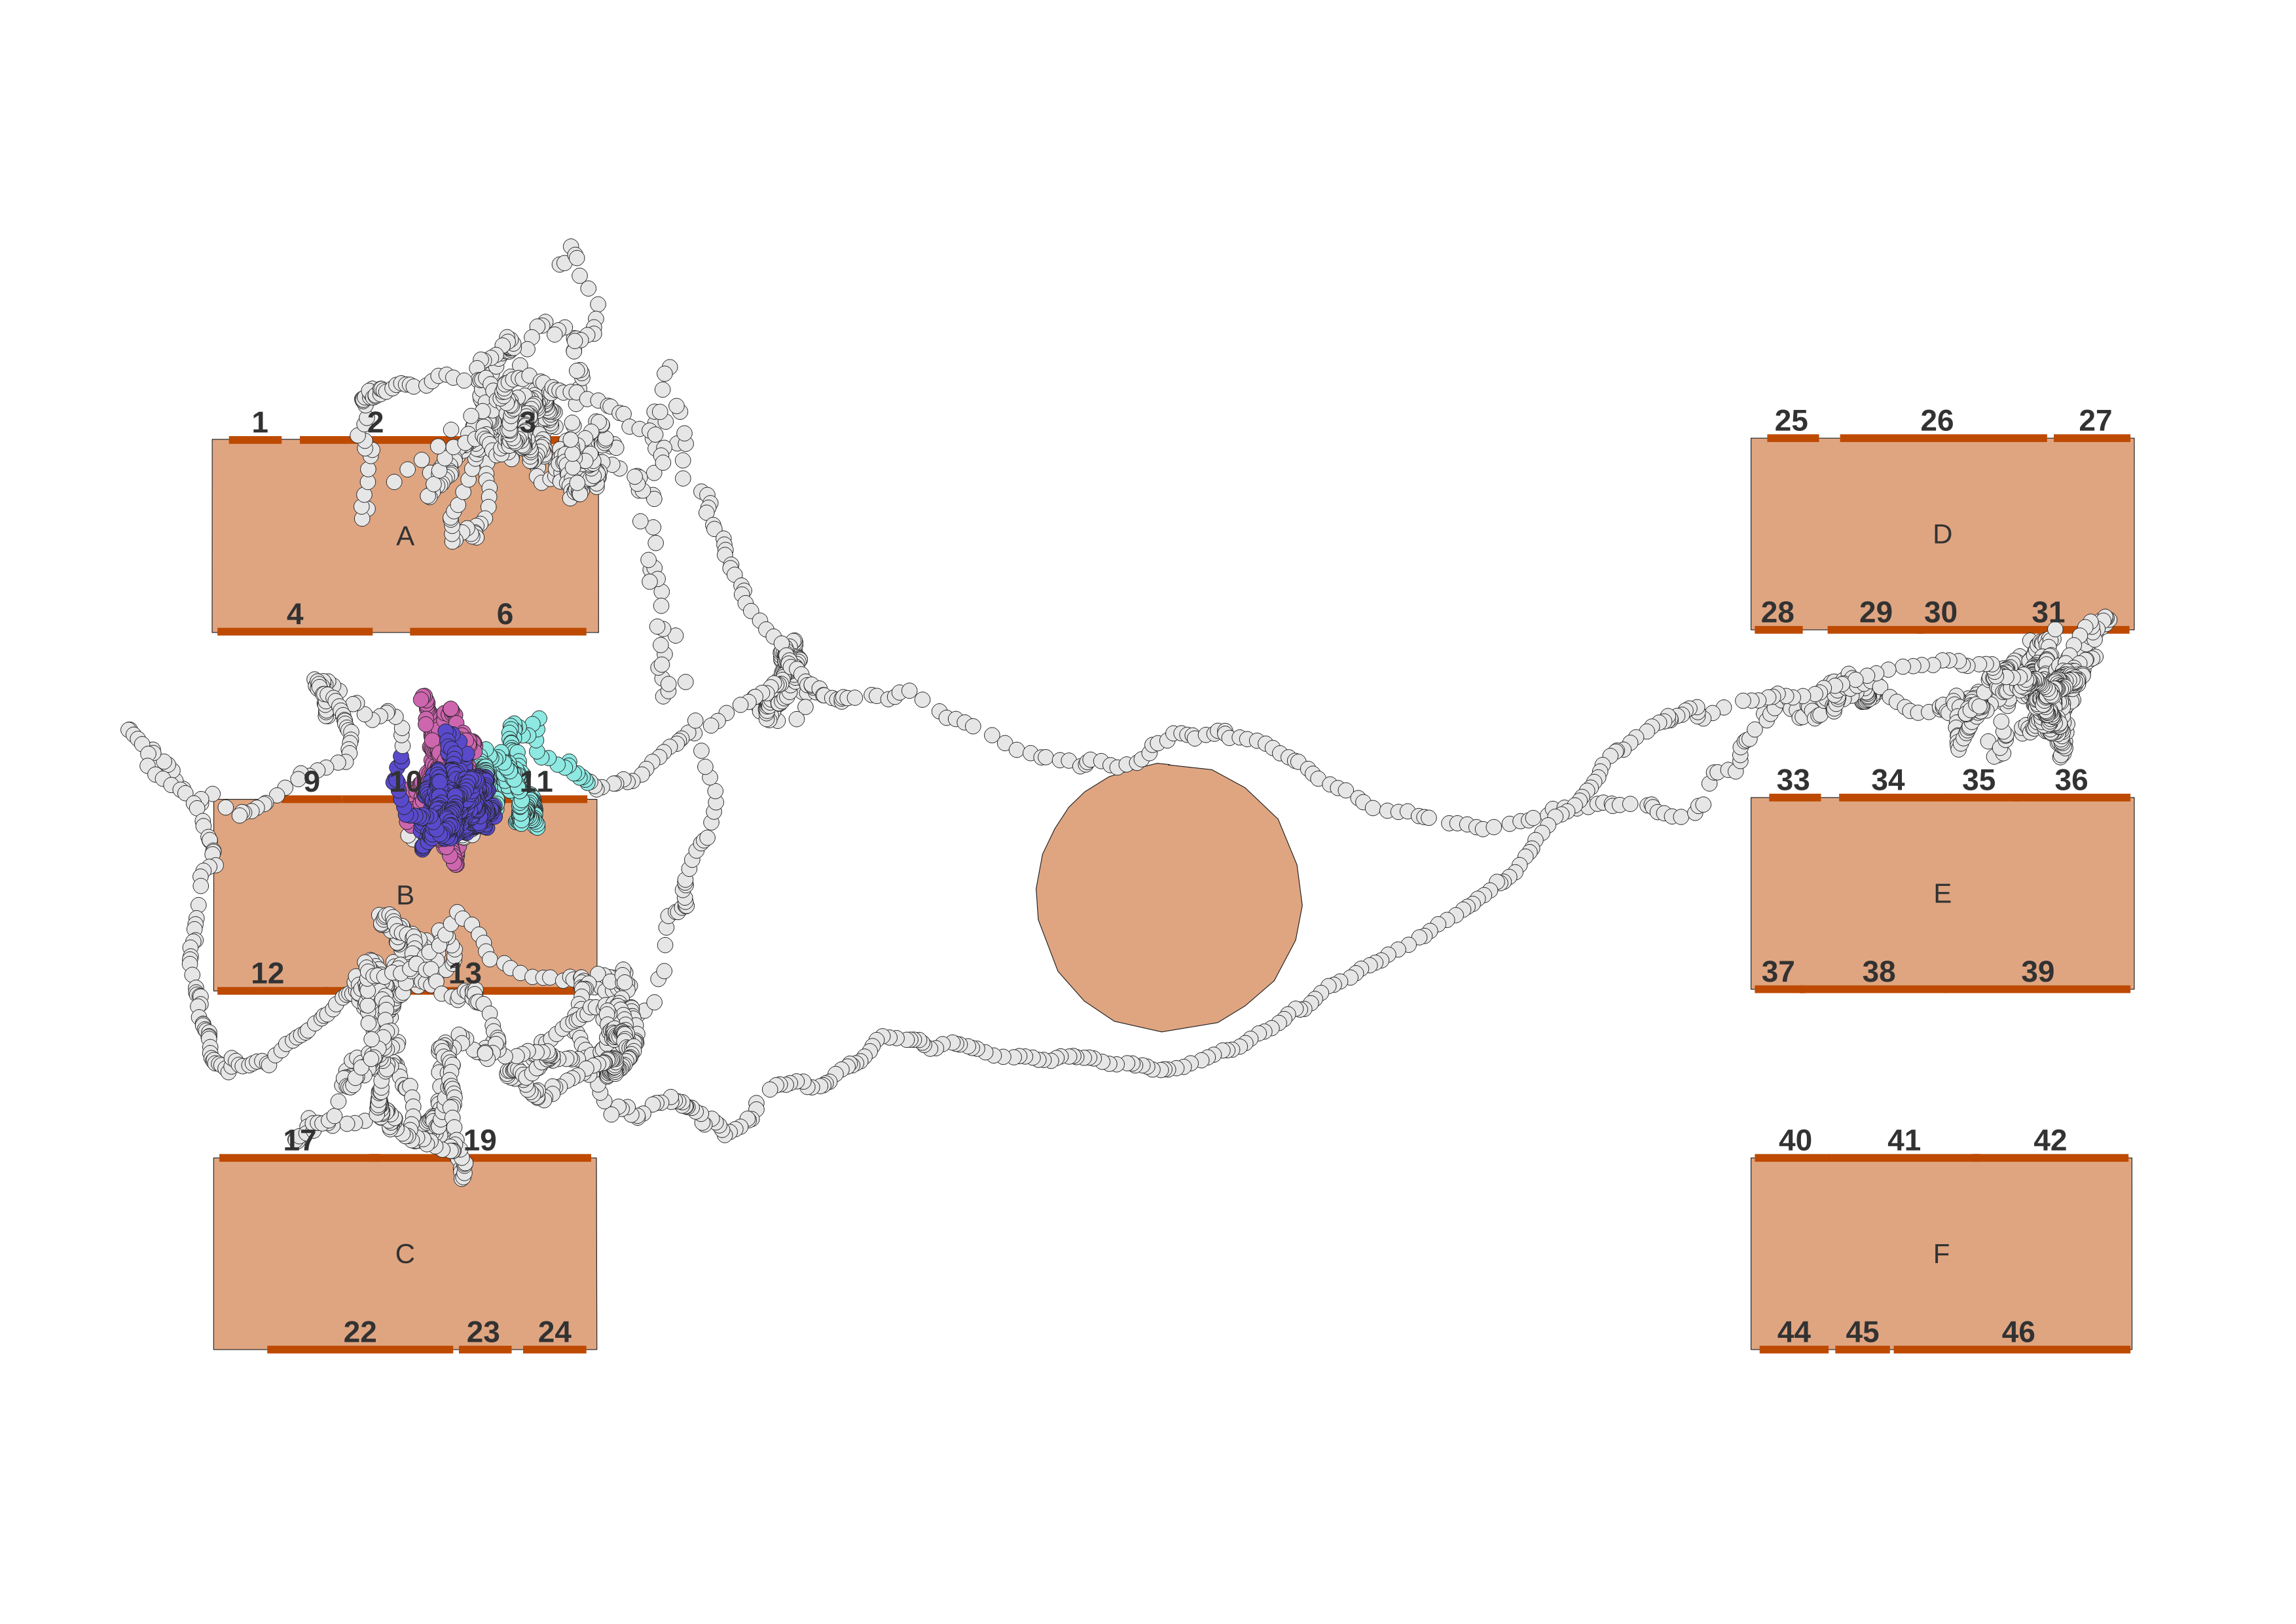
\includegraphics[width=\textwidth]{images/stop_points_p68_SOC_eps1_tau30_minMov05.png}
        \caption{Parametri: eps=1, tau=30, minMov=0.5. Fermate individuate: 3.}
        \label{stop_points_p68_SOC_eps1_tau30_minMov05}
    \end{subfigure}
    \hfill
    \caption{Punti di stop della persona 57 (a,b), della persona 67 (c,d) e della persona 68 (e,f), individuati con l'algoritmo SOC.}
    \label{stop_points_SOC}
\end{figure}


\begin{figure}[htb!]
    \centering
    \begin{subfigure}[b]{0.3\textwidth}
        \centering
        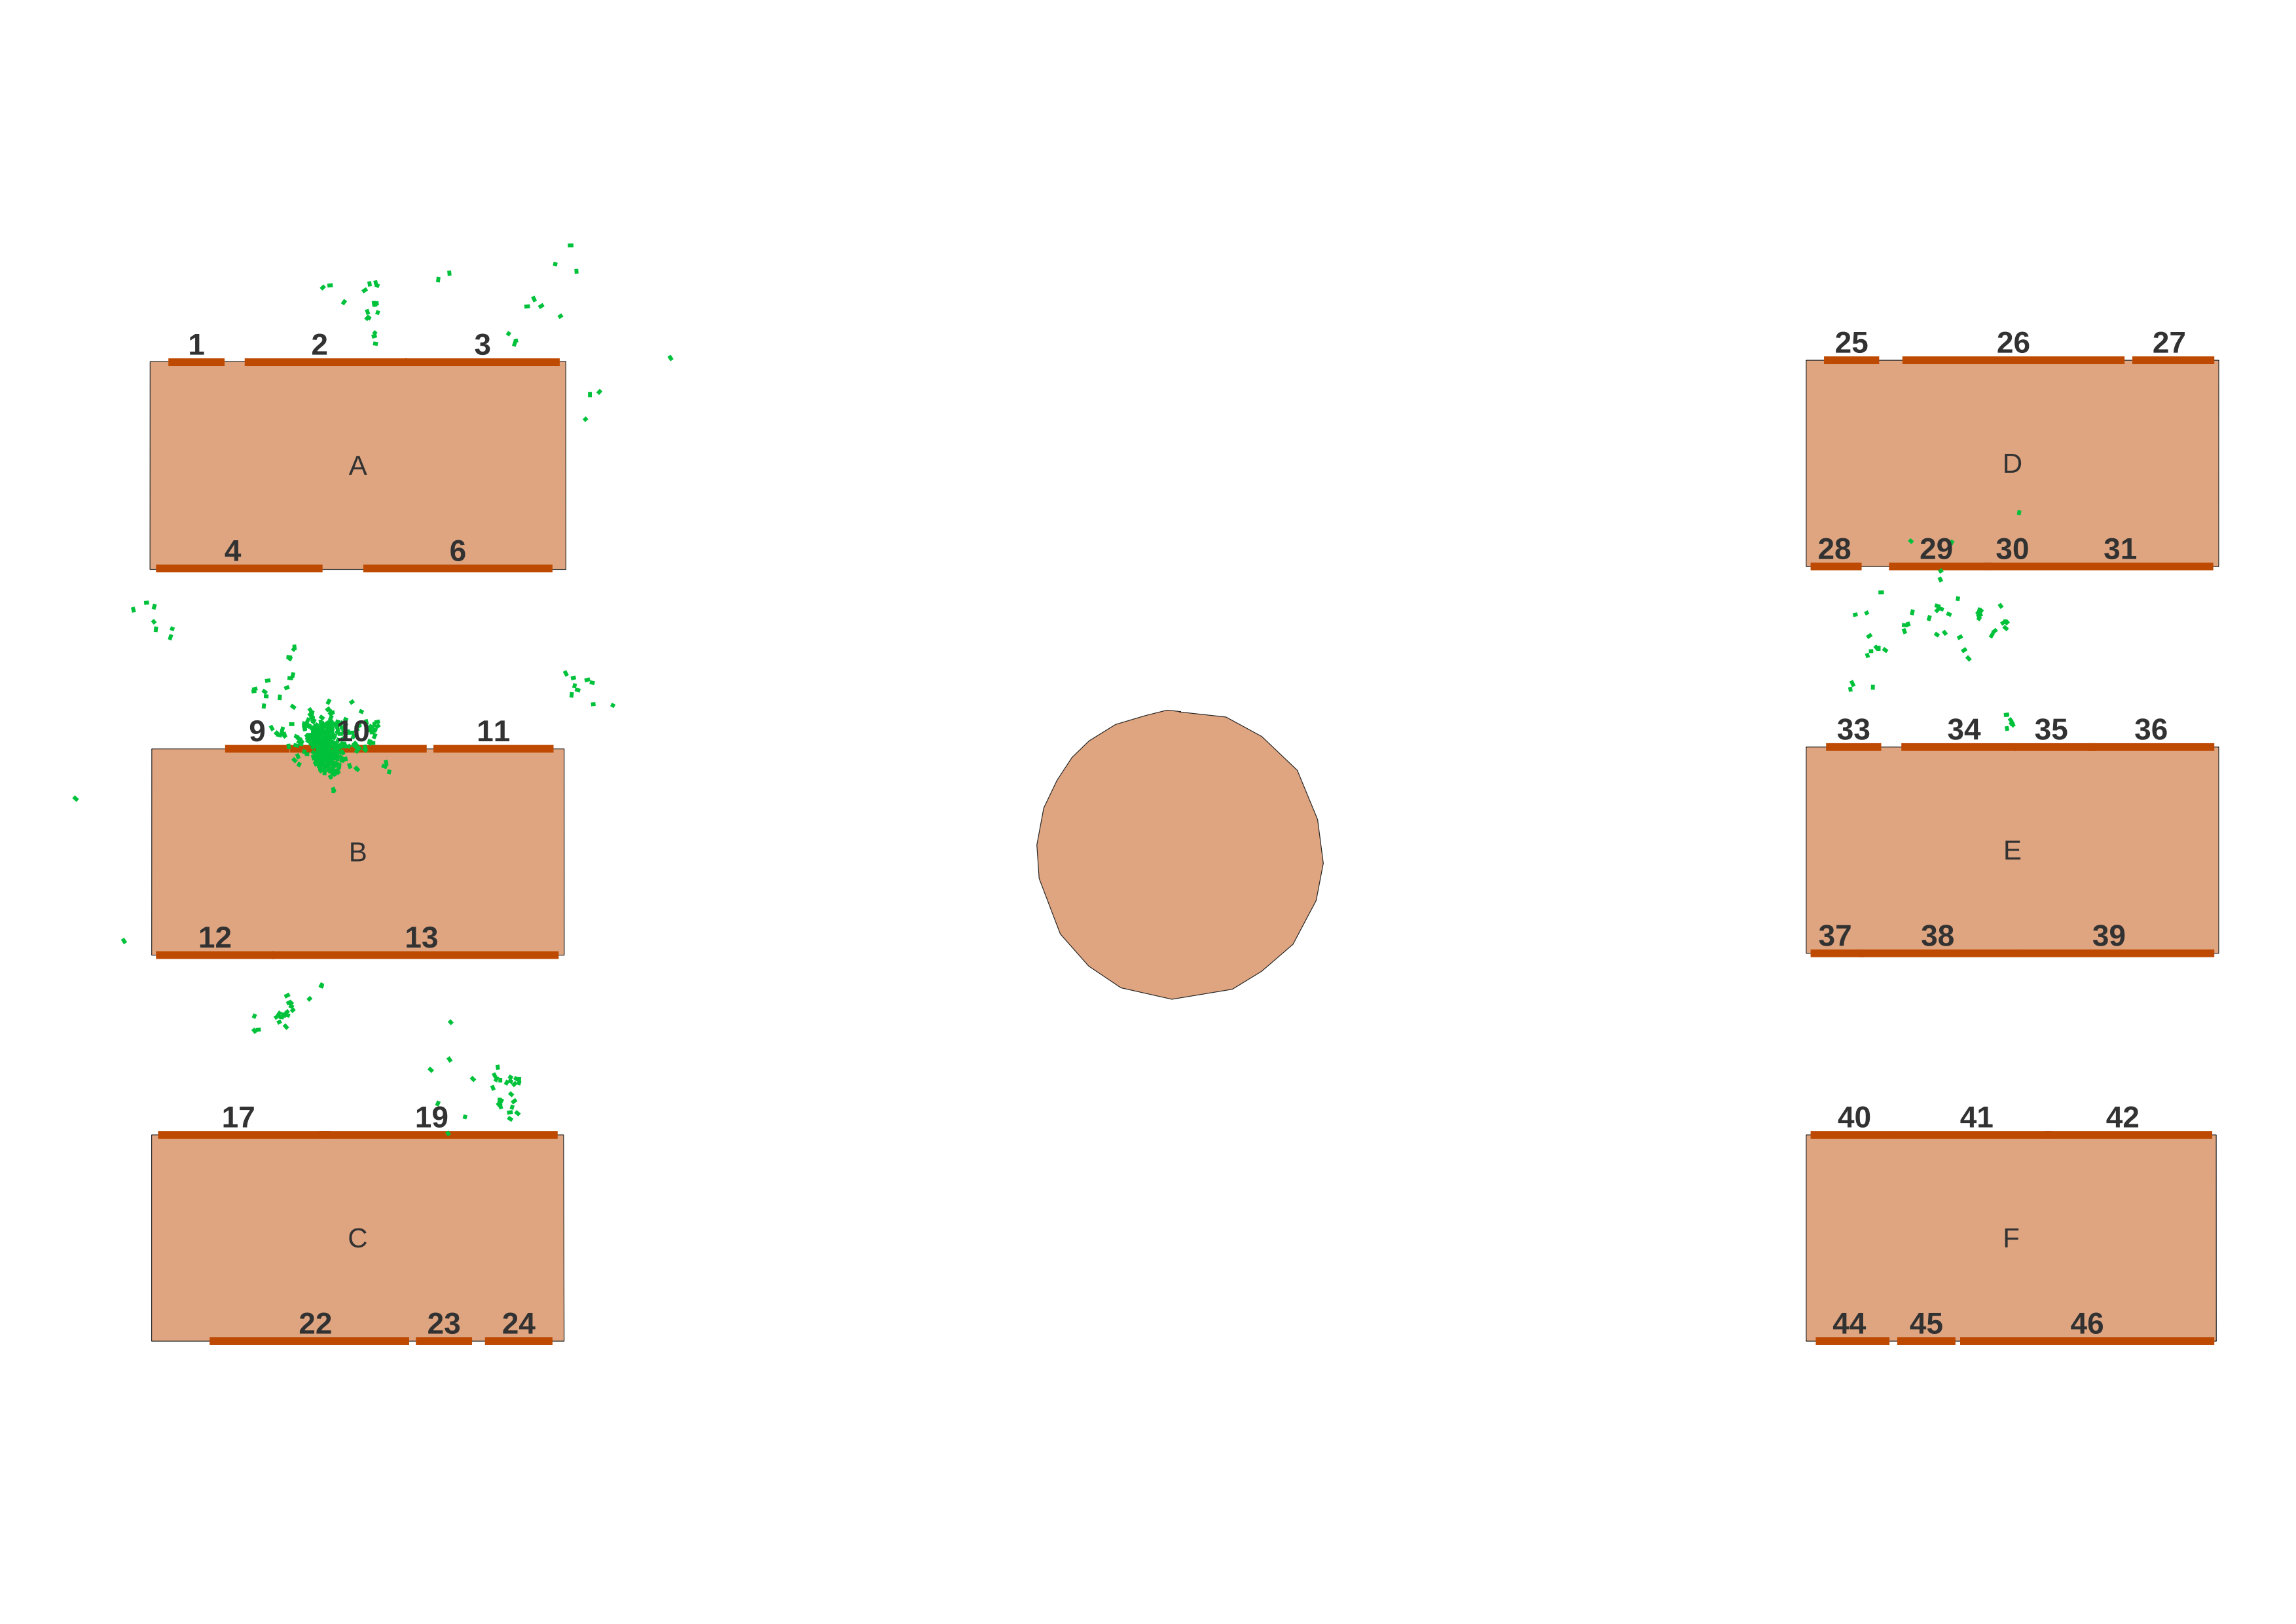
\includegraphics[width=\textwidth]{images/stop_points_p57_MSN.png}
        \caption{}
        \label{stop_segments_p57_MSN}
    \end{subfigure}
    \hfill
    \begin{subfigure}[b]{0.3\textwidth}
        \centering
        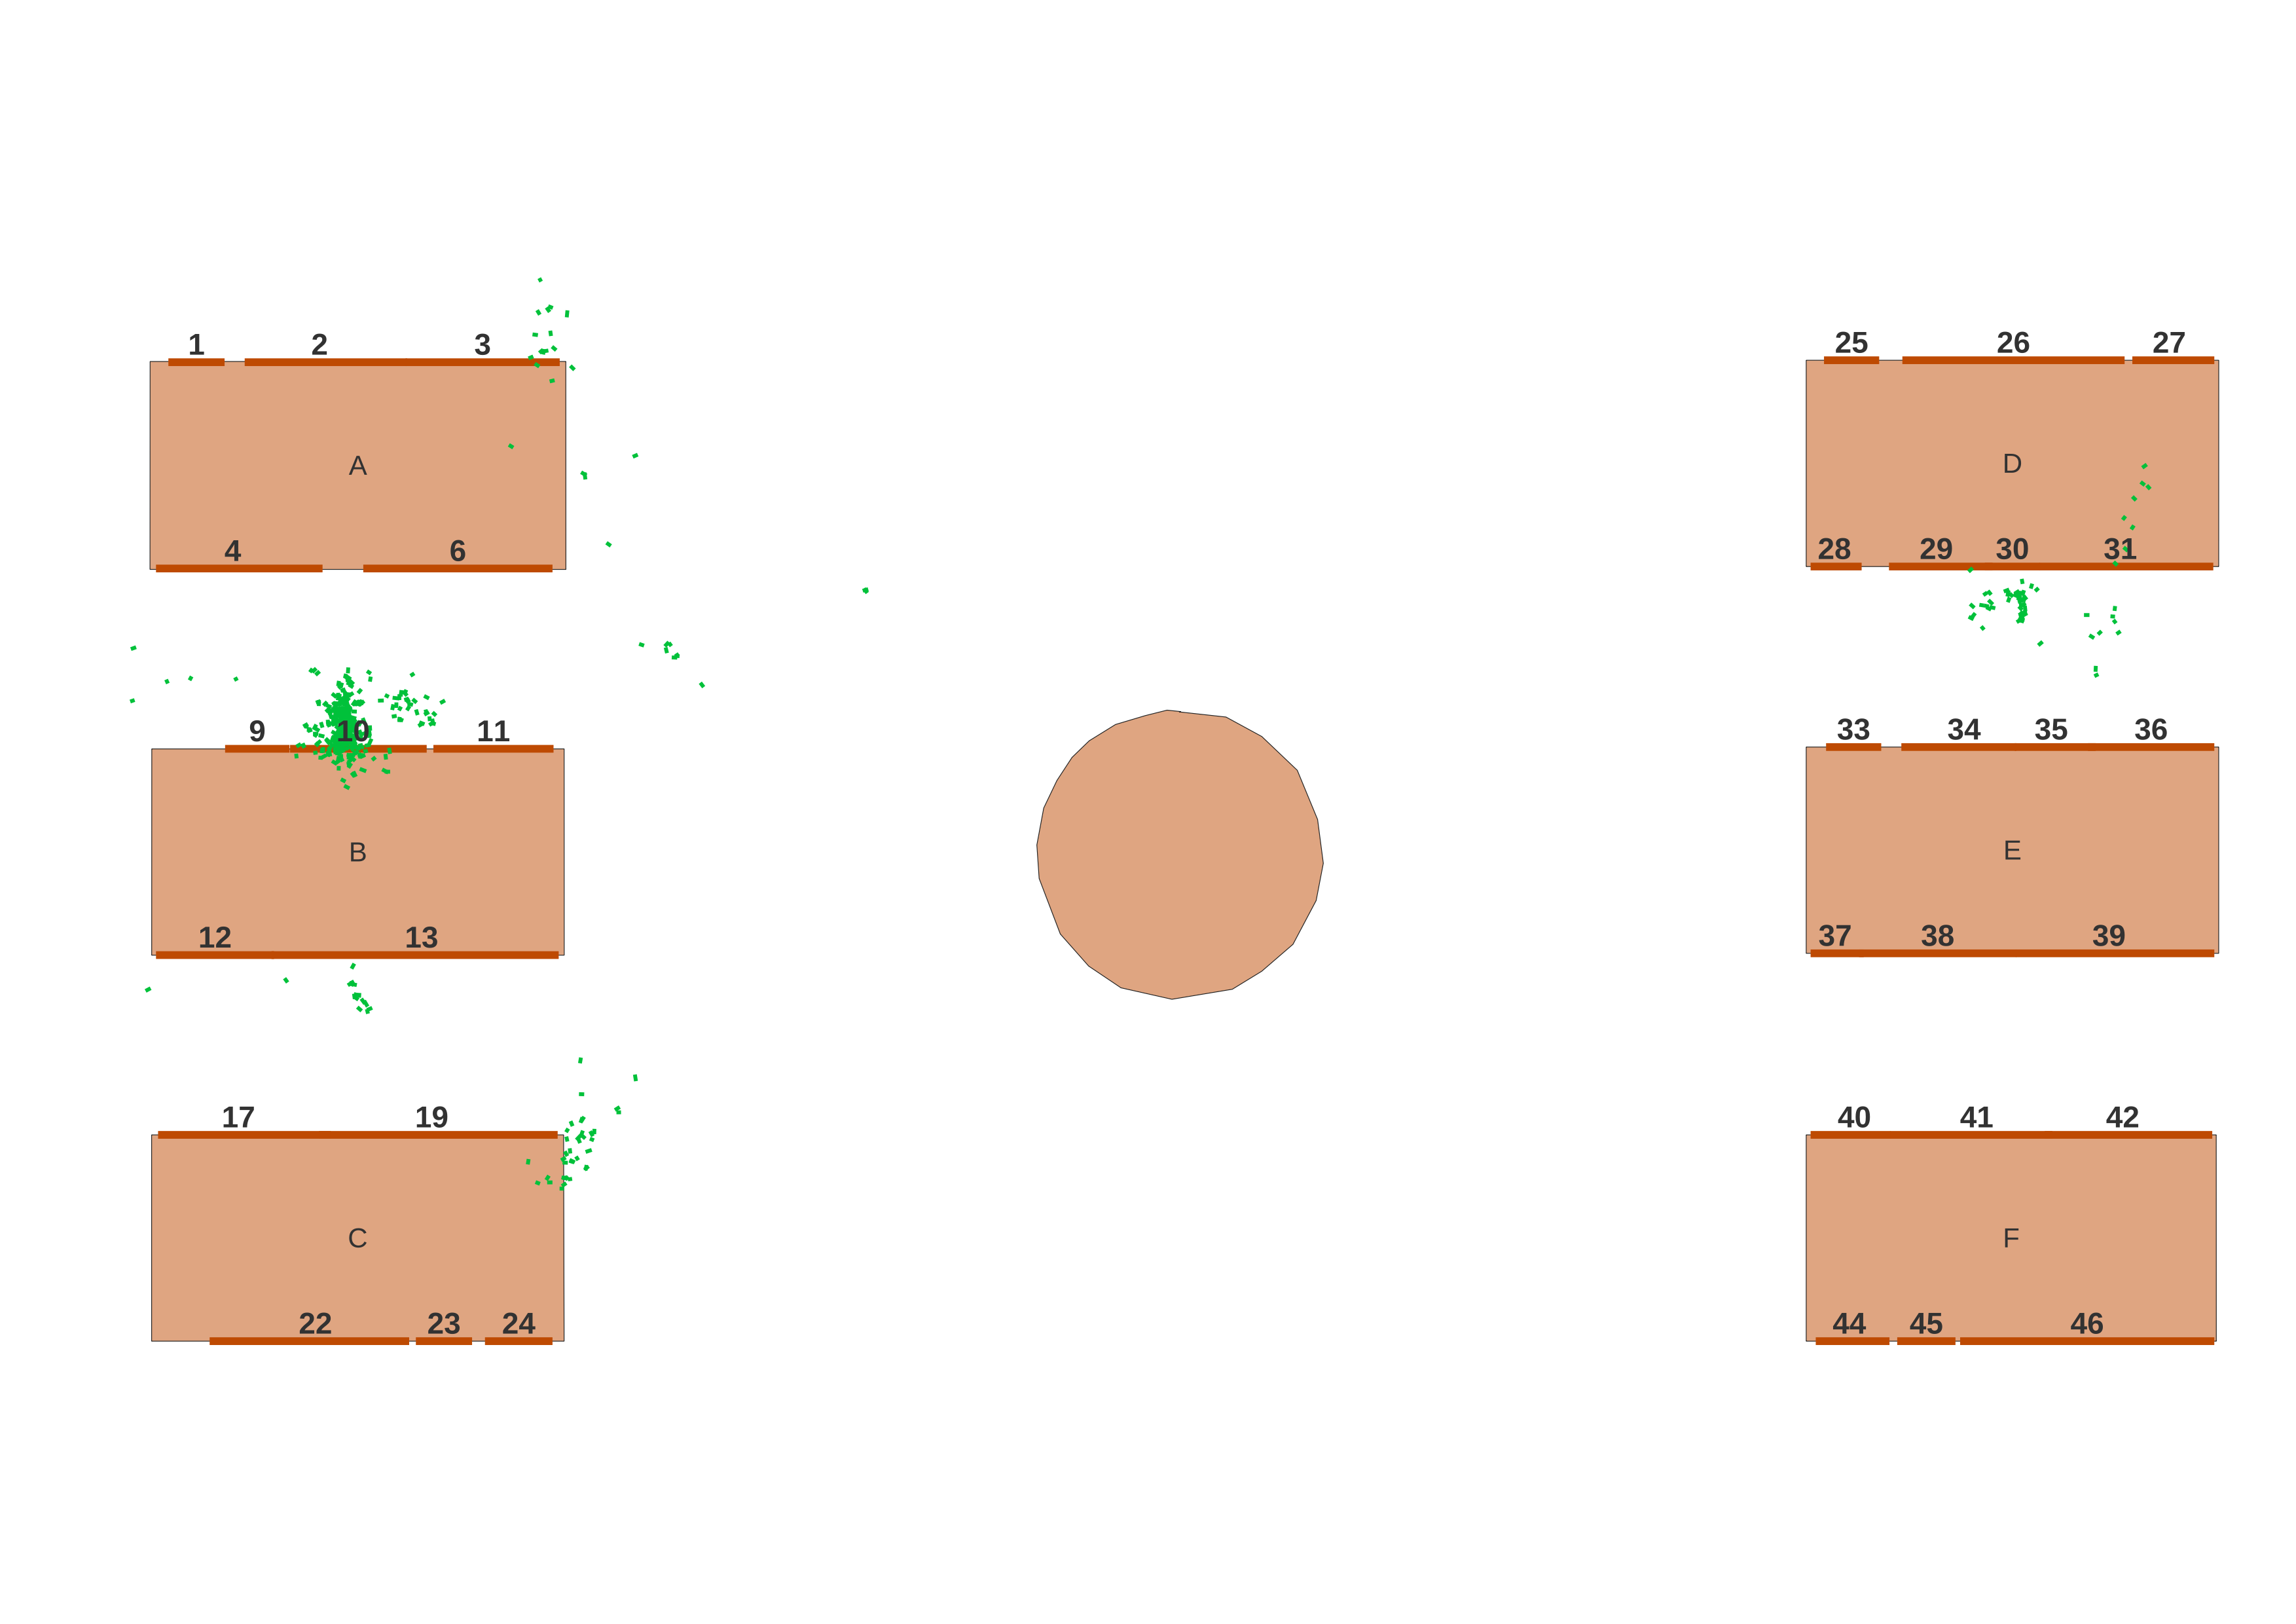
\includegraphics[width=\textwidth]{images/stop_points_p67_MSN.png}
        \caption{}
        \label{stop_segments_p67_MSN}
    \end{subfigure}
    \hfill
    \begin{subfigure}[b]{0.3\textwidth}
        \centering
        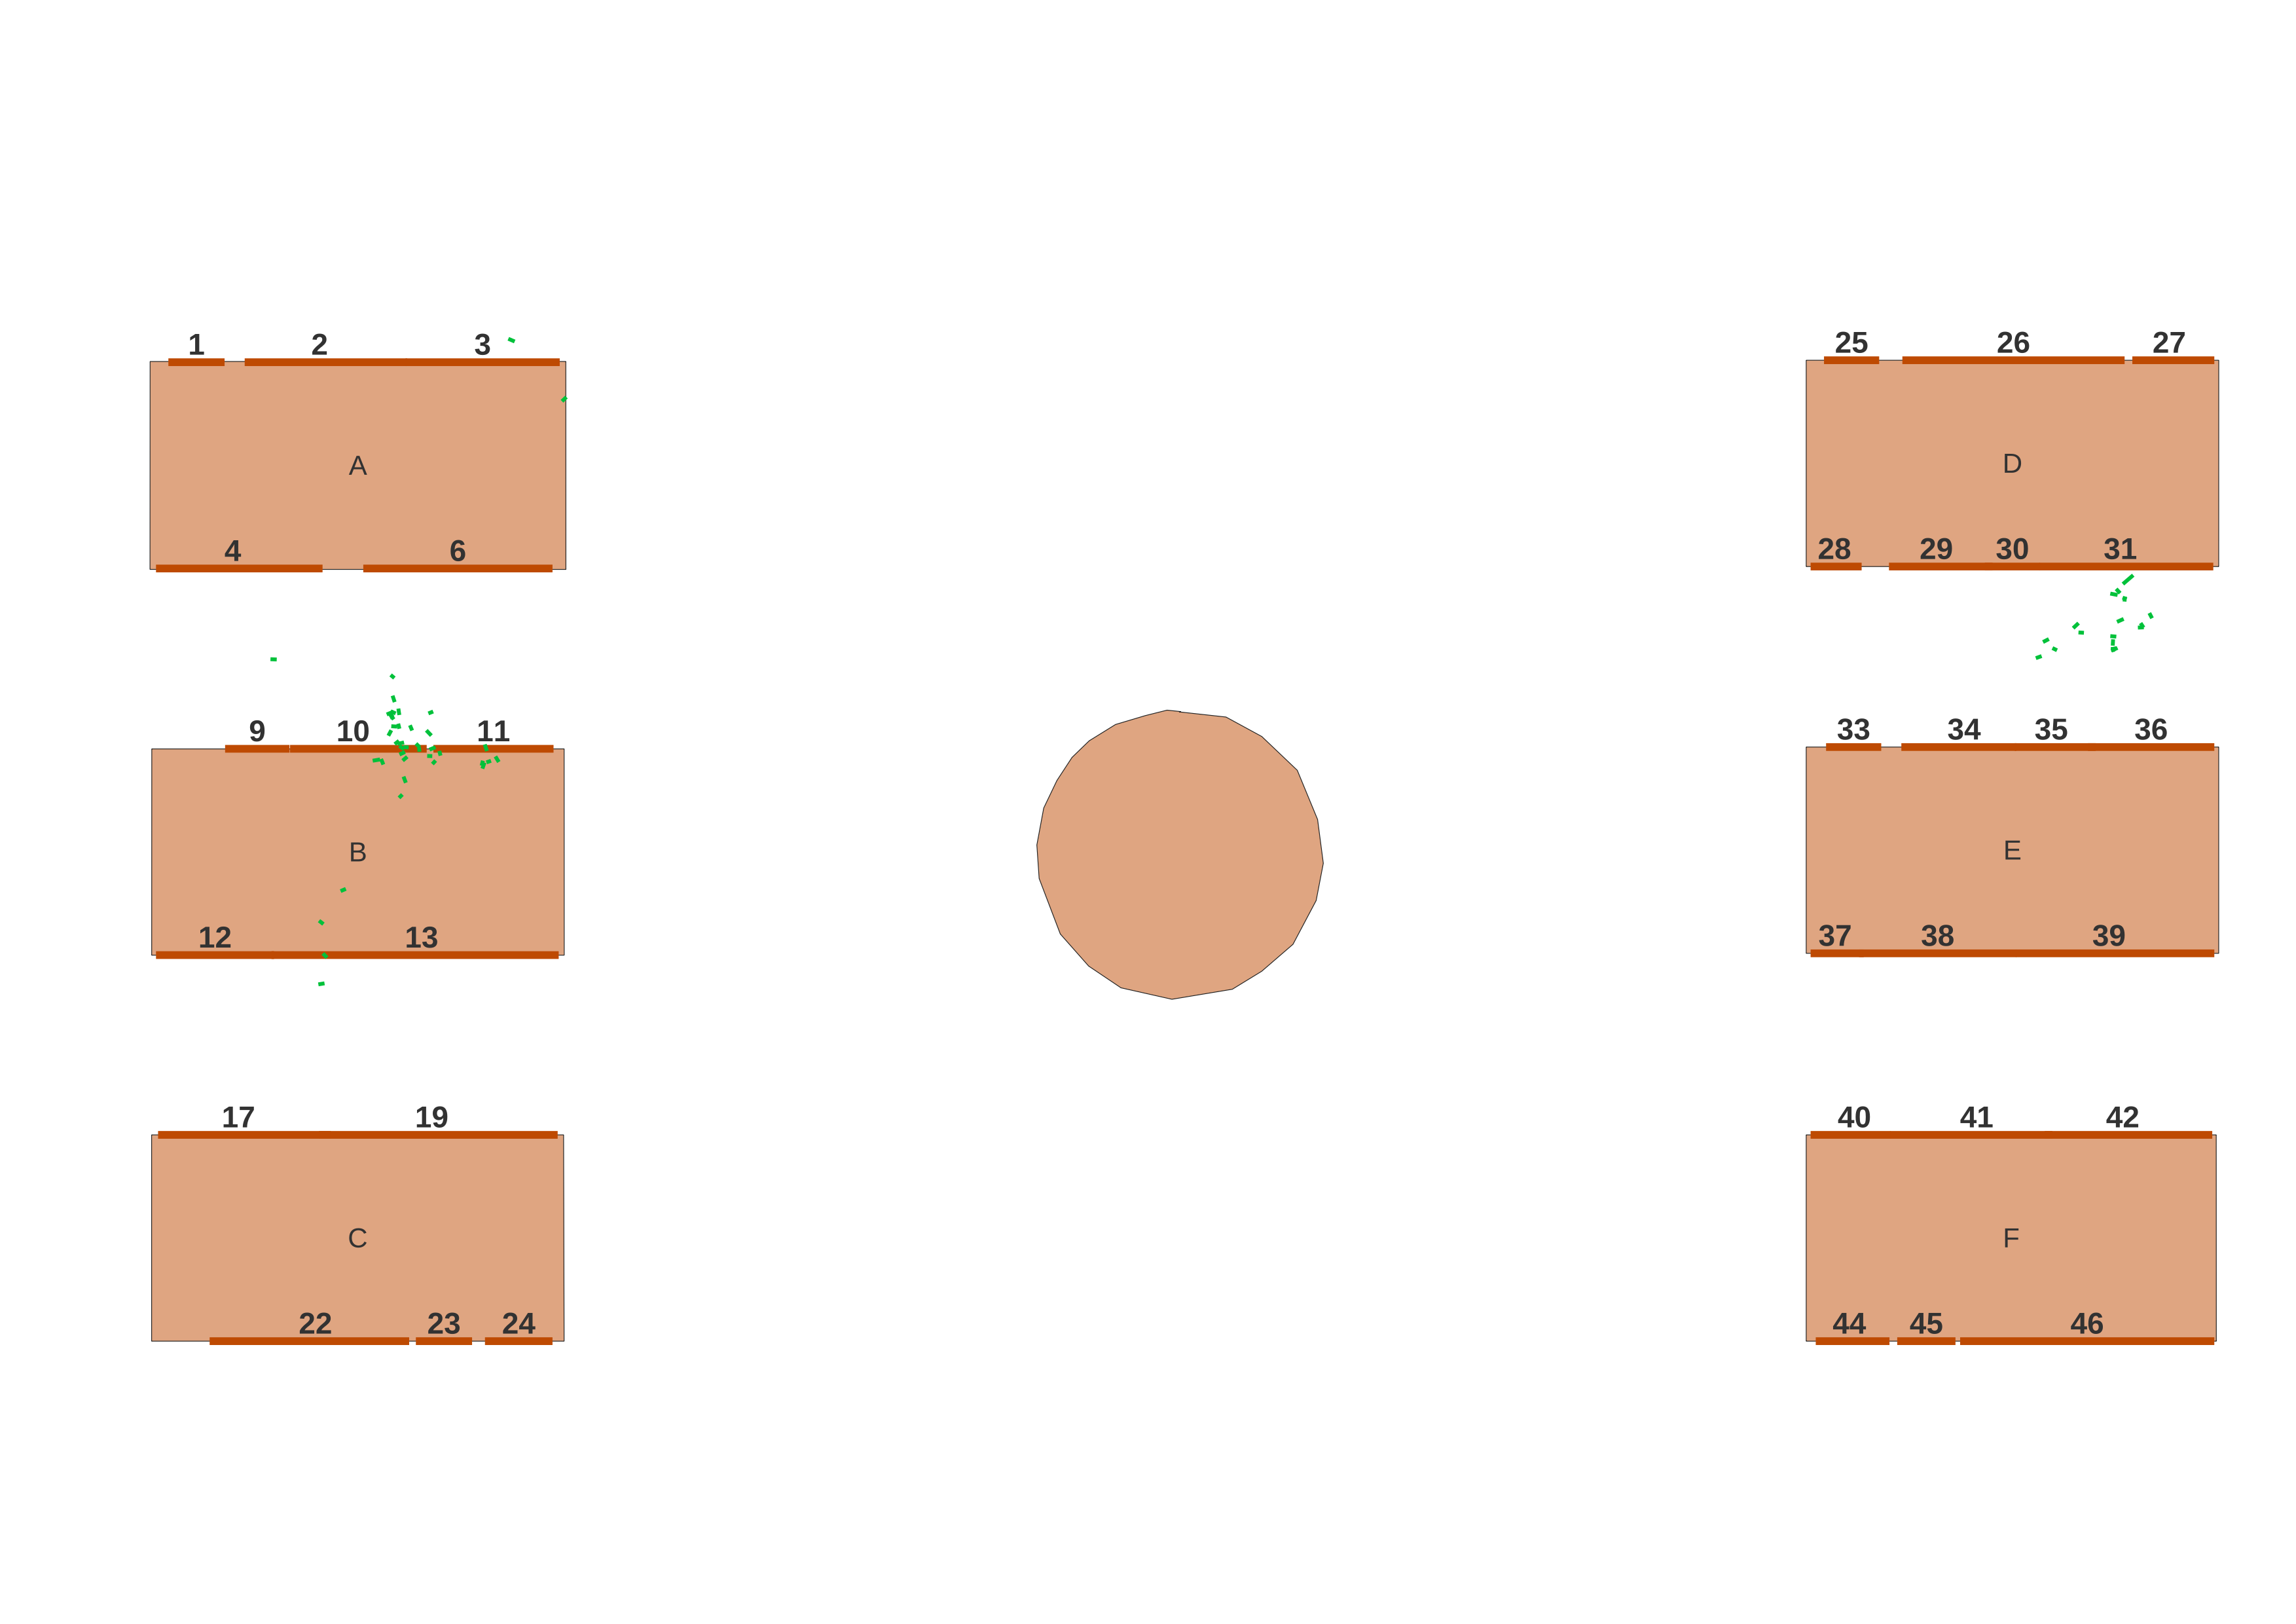
\includegraphics[width=\textwidth]{images/stop_points_p68_MSN.png}
        \caption{}
        \label{stop_segments_p68_MSN}
    \end{subfigure}
    \hfill
    \caption{Segmenti di stop della persona 57 (a), della persona 67 (b) e della persona 68 (c), individuati con l'algoritmo MSN.}
    \label{stop_segments_MSN}
\end{figure}

\clearpage

\section{Calcolo dei tempi di osservazione}\label{calcolo_tempi}
Parte delle analisi eseguite sui risultati dell'algoritmo SOC riguardano il calcolo dei seguenti tempi di osservazione:
\begin{enumerate}
    \item per ogni persona, calcolare per quanto tempo ha osservato ciascuna esibizione del museo, tenendo conto dei soli punti di fermata;
    \item per ogni esibizione del museo, calcolare il tempo totale di osservazione delle persone nei suoi pressi, tenendo conto dei soli punti di fermata.
\end{enumerate}
Nelle analisi abbiamo tenuto conto delle seguenti assunzioni:
\begin{itemize}
    \item un visitatore osserva un'esibizione se si trova a una distanza di al più 0.7 metri dalla stessa;
    \item un visitatore, dopo aver visitato un'esibizione, non torna a visitarla in un secondo momento.
\end{itemize}
Come prima cosa abbiamo creato dei buffer di raggio $0.7$ metri intorno alle geometrie delle esibizioni, come mostrato in Figura \ref{tables_with_exhibits_buffer}, per poter tenere nelle analisi solo dei punti che intersecano tali buffer.
Successivamente, abbiamo disambiguato l'esibizione a cui fanno riferimento i punti che intersecano due o più esibizioni, considerando l'esibizione che ha distanza punto-centroide dell'esibizione più corta.
Poi, abbiamo calcolato i tempi di visita relativi a ciascun visitatore e i tempi totali di visita delle esibizioni, ottenendo i risultati in Tabella \ref{persons_time_visiting} e in Tabella \ref{exhibits_time_visiting}.
Infine, per tener conto anche della presenza di rumore nei dati, abbiamo ripetuto le analisi considerando tutti i punti di tutti i cluster i cui centroidi intersecano i buffer delle esibizioni, ottenendo i risultati in Tabella \ref{persons_time_visiting_cluster} e in Tabella \ref{exhibits_time_visiting_cluster}.

\begin{figure}[htb!]
    \centering
    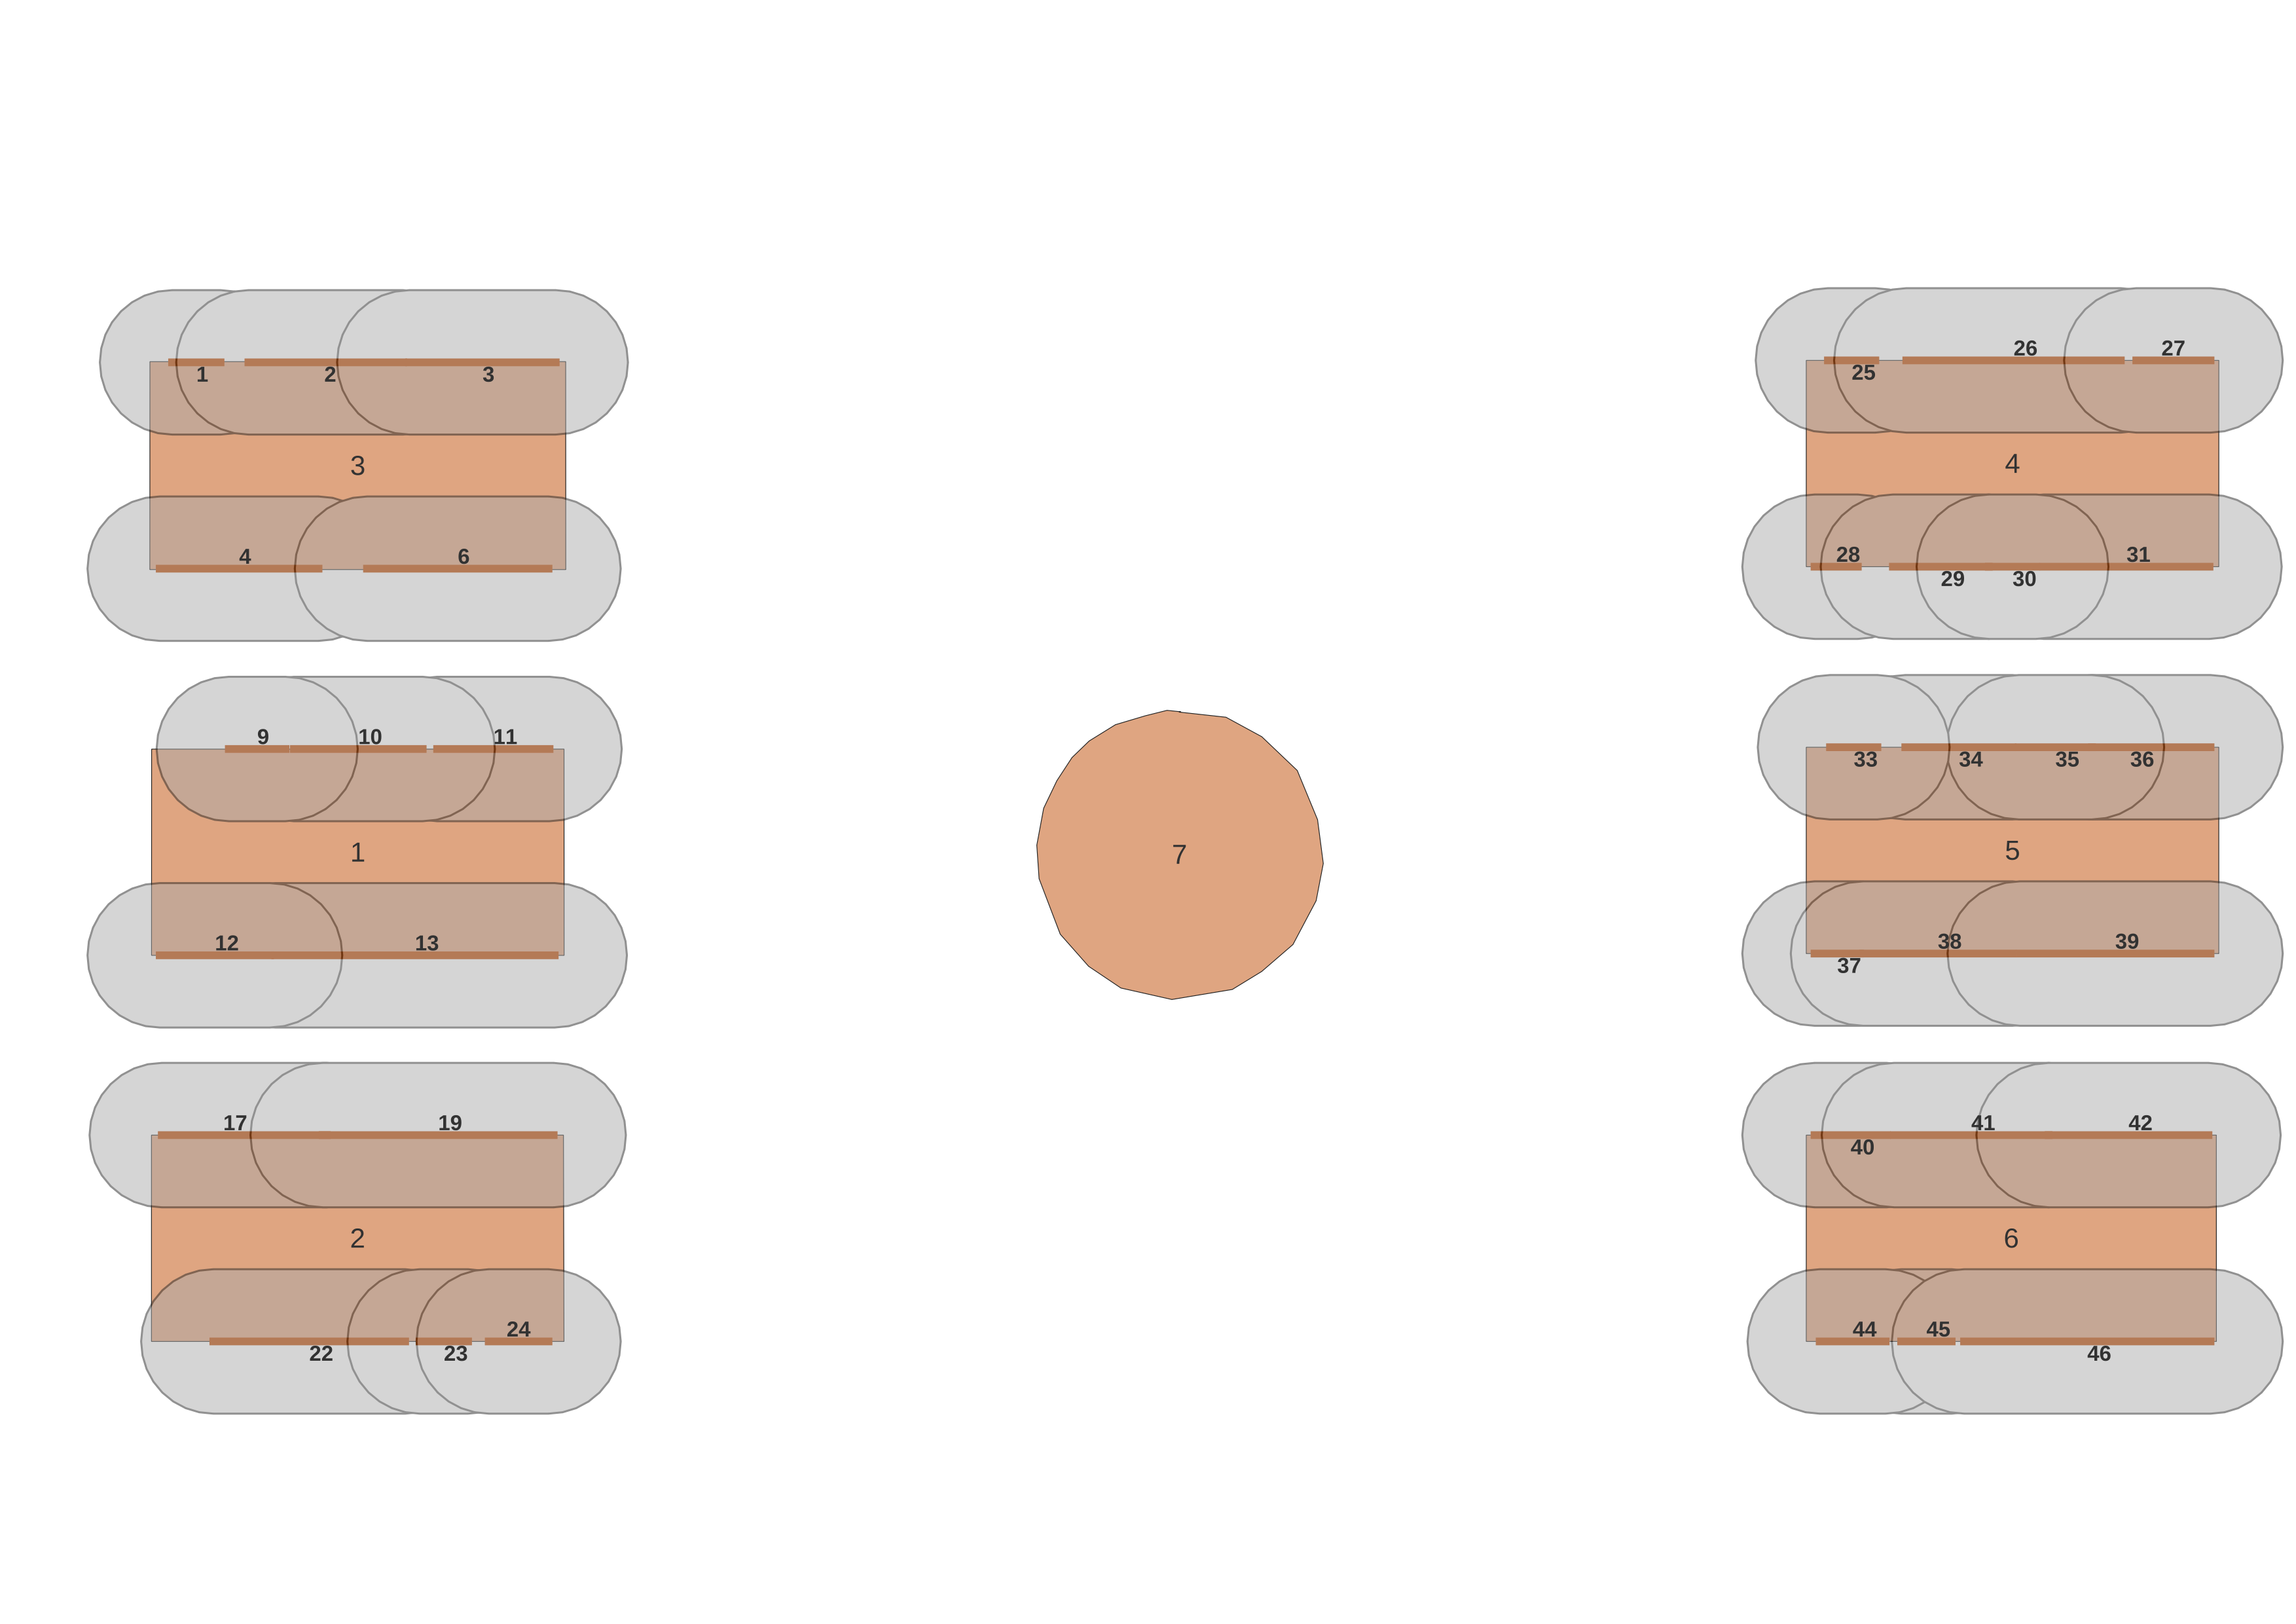
\includegraphics[width=0.35\textwidth]{images/tables_with_exhibits_buffer.png}
    \caption{Buffer di raggio 0.7 delle esibizioni.}
    \label{tables_with_exhibits_buffer}
\end{figure}

\begin{table}[!ht]
    \centering
    \begin{tabular}{|c|c|c|}
        \hline
        \textbf{Visitatore} & \textbf{Esibizione} & \textbf{Tempo di visita} \\ \hline
        57                  & 2.00                & 18.75                    \\ \hline
        57                  & 3.00                & 15.07                    \\ \hline
        57                  & 9.00                & 39.20                    \\ \hline
        57                  & 10.00               & 284.75                   \\ \hline
        57                  & 11.00               & 0.07                     \\ \hline
        57                  & 12.00               & 15.25                    \\ \hline
        57                  & 13.00               & 4.82                     \\ \hline
        57                  & 29.00               & 24.07                    \\ \hline
        57                  & 30.00               & 20.74                    \\ \hline
        67                  & 3.00                & 37.24                    \\ \hline
        67                  & 9                   & 5.85                     \\ \hline
        67                  & 10                  & 310.78                   \\ \hline
        67                  & 11                  & 8.25                     \\ \hline
        67                  & 29                  & 2.86                     \\ \hline
        67                  & 30                  & 30.53                    \\ \hline
        67                  & 31                  & 17.10                    \\ \hline
        68                  & 3                   & 2.43                     \\ \hline
        68                  & 6                   & 0.07                     \\ \hline
        68                  & 10                  & 204.66                   \\ \hline
        68                  & 11                  & 116.69                   \\ \hline
        68                  & 12                  & 0.86                     \\ \hline
        68                  & 13                  & 17.46                    \\ \hline
        68                  & 30                  & 2.32                     \\ \hline
        68                  & 31                  & 45.70                    \\ \hline
        68                  & 35                  & 0.57                     \\ \hline
        68                  & 36                  & 4.14                     \\ \hline
    \end{tabular}
    \caption{Tempo di visita delle esibizioni per ciascun visitatore.}
    \label{persons_time_visiting}
\end{table}

\begin{table}[!ht]
    \centering
    \begin{tabular}{|c|c|c|}
        \hline
        \textbf{Visitatore} & \textbf{Esibizione} & \textbf{Tempo di visita} \\ \hline
        57                  & 2.00                & 24.17                    \\ \hline
        57                  & 3.00                & 7.93                     \\ \hline
        57                  & 10.00               & 330.42                   \\ \hline
        57                  & 12.00               & 20.67                    \\ \hline
        57                  & 29.00               & 25.32                    \\ \hline
        57                  & 30.00               & 20.74                    \\ \hline
        67                  & 3.00                & 37.24                    \\ \hline
        67                  & 10.00               & 327.35                   \\ \hline
        67                  & 30.00               & 34.74                    \\ \hline
        67                  & 31.00               & 17.10                    \\ \hline
        68                  & 3.00                & 2.43                     \\ \hline
        68                  & 10.00               & 189.06                   \\ \hline
        68                  & 11.00               & 141.29                   \\ \hline
        68                  & 13                  & 18.75                    \\ \hline
        68                  & 31                  & 67.13                    \\ \hline
        67                  & 31                  & 17.10                    \\ \hline
        68                  & 3                   & 2.43                     \\ \hline
        68                  & 6                   & 0.07                     \\ \hline
        68                  & 10                  & 204.66                   \\ \hline
        68                  & 11                  & 116.69                   \\ \hline
        68                  & 12                  & 0.86                     \\ \hline
        68                  & 13                  & 17.46                    \\ \hline
        68                  & 30                  & 2.32                     \\ \hline
        68                  & 31                  & 45.70                    \\ \hline
        68                  & 35                  & 0.57                     \\ \hline
        68                  & 36                  & 4.14                     \\ \hline
    \end{tabular}
    \caption{Tempo di visita delle esibizioni per ciascun visitatore, considerando tutti i punti dei cluster i cui centroidi intersecano i buffer delle esibizioni.}
    \label{persons_time_visiting_cluster}
\end{table}

\begin{table}[!ht]
    \centering
    \begin{tabular}{|c|c|}
        \hline
        \textbf{Esibizione} & \textbf{Tempo di visita} \\ \hline
        2                   & 18.75                    \\ \hline
        3                   & 54.74                    \\ \hline
        6                   & 0.07                     \\ \hline
        9                   & 45.06                    \\ \hline
        10                  & 800.19                   \\ \hline
        11                  & 125.00                   \\ \hline
        12                  & 16.10                    \\ \hline
        13                  & 22.28                    \\ \hline
        29                  & 26.92                    \\ \hline
        30                  & 53.59                    \\ \hline
        31                  & 62.81                    \\ \hline
        35                  & 0.57                     \\ \hline
        36                  & 4.14                     \\ \hline
    \end{tabular}
    \caption{Tempo totale di visita delle esibizioni.}
    \label{exhibits_time_visiting}
\end{table}

\begin{table}[!ht]
    \centering
    \begin{tabular}{|c|c|}
        \hline
        \textbf{Esibizione} & \textbf{Tempo di visita} \\ \hline
        2                   & 24.17                    \\ \hline
        3                   & 47.60                    \\ \hline
        10                  & 846.82                   \\ \hline
        11                  & 141.29                   \\ \hline
        12                  & 20.67                    \\ \hline
        13                  & 18.75                    \\ \hline
        29                  & 25.32                    \\ \hline
        30                  & 55.49                    \\ \hline
        31                  & 84.23                    \\ \hline
    \end{tabular}
    \caption{Tempo totale di visita delle esibizioni, considerando tutti i punti dei cluster i cui centroidi intersecano i buffer delle esibizioni.}
    \label{exhibits_time_visiting_cluster}
\end{table}

\section{Osservazione congiunta dei visitatori}
L'analisi si conclude con il trovare, per ogni esibizione del museo, il numero di persone che la osservano congiuntamente nel tempo.
Per rispondere a questo quesito ci siamo serviti di MobilityDB \cite{MobilityDBTODS2020}, una piattaforma per la gestione e l'analisi di traiettorie geospaziali.
MobilityDB estende PostgreSQL e PostGIS con tipi di dato temporali (\emph{ttype}) e geometrie temporali (\emph{tgeom}) che semplificano l'analisi delle traiettorie.
Dai punti disambiguati che intersecano i buffer delle esibizioni abbiamo creato le geometrie temporali che rappresento i punti di fermata davanti alle esibizioni di ciascun visitatore.
Su queste geometrie abbiamo poi applicato la funzione \emph{tcount}, la quale esegue l'interpolazione \emph{stepwise} per descrivere l'evoluzione temporale dei valori.
Nel nostro caso, viene restituito un \emph{tint} che rappresenta la variazione nel tempo del numero di visitatori che osservano l'esibizione (Figura \ref{person_over_time}).
La struttura delle tabelle utilizzate, la query eseguita e il diagramma a blocchi riassuntivo sono descritti nella Sezione \ref{section_query}.
Un esempio di \emph{tint} è data dalla sequenza temporale: \\
{[1@2021-12-13 12:08:52.424+01, 2@2021-12-13 12:08:55.537+01, 3@2021-12-13 12:09:25.787+01, 3@2021-12-13 12:14:20.27+01], (2@2021-12-13 12:14:20.2\\7+01, 2@2021-12-13 12:14:20.349+01], (1@2021-12-13 12:14:20.349+01, 1@20\\21-12-13 12:14:24.962+01]}.\\
Il valore di una sequenza temporale è interpretato assumendo che l'intervallo di tempo definito da ciascuna coppia di valori consecutivi sia chiuso a sinistra e aperto a destra, a meno che non siano la prima o l'ultima istanza della sequenza: in quel caso si applica il tipo di intervallo dell'intera sequenza.
Quindi la precedente sequenza viene interpretata nel seguente modo:
\begin{itemize}
    \item l'esibizione è osservata da 1 visitatore dall'istante 2021-12-13 12:08:52.\\424+01 all'istante precedente a 2021-12-13 12:08:55.537+01;
    \item l'esibizione è osservata da 2 visitatori dall'istante 2021-12-13 12:08:55.\\537+01 all'istante precedente a 2021-12-13 12:09:25.787+01;
    \item l'esibizione è osservata da 3 visitatori dall'istante 2021-12-13 12:09:25.\\787+01 all'istante 2021-12-13 12:14:20.27+01;
    \item l'esibizione ritorna ad essere visitata da 2 visitatori dall'istante successivo a 2021-12-13 12:14:20.27+01 all'istante 2021-12-13 12:14:20.349+01.
\end{itemize}

\begin{figure}[!h]
    \centering
    \resizebox{0.7\textwidth}{!}{%
        \tikzset{every picture/.style={line width=0.75pt}} %set default line width to 0.75pt        

    \begin{tikzpicture}[x=0.75pt,y=0.75pt,yscale=-1,xscale=1]
        %uncomment if require: \path (0,1104); %set diagram left start at 0, and has height of 1104

        %Straight Lines [id:da4285063956632724] 
        \draw [line width=0.75]    (155.21,1044.82) -- (155.21,15) ;
        \draw [shift={(155.21,13)}, rotate = 90] [color={rgb, 255:red, 0; green, 0; blue, 0 }  ][line width=0.75]    (10.93,-3.29) .. controls (6.95,-1.4) and (3.31,-0.3) .. (0,0) .. controls (3.31,0.3) and (6.95,1.4) .. (10.93,3.29)   ;
        %Straight Lines [id:da16719921511658842] 
        \draw [line width=0.75]    (155.21,1044.82) -- (608.23,1044.82) ;
        \draw [shift={(610.23,1044.82)}, rotate = 180] [color={rgb, 255:red, 0; green, 0; blue, 0 }  ][line width=0.75]    (10.93,-3.29) .. controls (6.95,-1.4) and (3.31,-0.3) .. (0,0) .. controls (3.31,0.3) and (6.95,1.4) .. (10.93,3.29)   ;
        %Straight Lines [id:da7351868924662883] 
        \draw [line width=0.75]  [dash pattern={on 0.84pt off 2.51pt}]  (181.95,1044.62) -- (181.95,38.83) ;
        %Straight Lines [id:da0481202130494327] 
        \draw [line width=0.75]  [dash pattern={on 0.84pt off 2.51pt}]  (216.74,1044.62) -- (216.74,36.98) ;
        %Straight Lines [id:da9228474331817789] 
        \draw [line width=0.75]  [dash pattern={on 0.84pt off 2.51pt}]  (251.53,1044.62) -- (251.53,39.75) ;
        %Straight Lines [id:da9466132010483053] 
        \draw [line width=0.75]  [dash pattern={on 0.84pt off 2.51pt}]  (286.32,1044.62) -- (286.32,37.91) ;
        %Straight Lines [id:da24183906778422548] 
        \draw [line width=0.75]  [dash pattern={on 0.84pt off 2.51pt}]  (321.1,1044.62) -- (321.1,37.91) ;
        %Straight Lines [id:da8096611504325302] 
        \draw [line width=0.75]  [dash pattern={on 0.84pt off 2.51pt}]  (355.89,1044.62) -- (355.89,38.8) ;
        %Straight Lines [id:da4891313983154093] 
        \draw [line width=0.75]  [dash pattern={on 0.84pt off 2.51pt}]  (390.68,1044.62) -- (390.68,39.75) ;
        %Straight Lines [id:da03406843300524032] 
        \draw [line width=0.75]  [dash pattern={on 0.84pt off 2.51pt}]  (425.47,1044.62) -- (425.47,36.98) ;
        %Straight Lines [id:da18686644469791314] 
        \draw [line width=0.75]  [dash pattern={on 0.84pt off 2.51pt}]  (460.26,1044.62) -- (460.26,39.75) ;
        %Straight Lines [id:da6803761167757145] 
        \draw [line width=0.75]  [dash pattern={on 0.84pt off 2.51pt}]  (495.05,1044.62) -- (495.05,37.66) ;
        %Straight Lines [id:da5818994143269787] 
        \draw [line width=0.75]  [dash pattern={on 0.84pt off 2.51pt}]  (529.84,1044.62) -- (529.84,36.98) ;
        %Straight Lines [id:da7848156626347245] 
        \draw [line width=0.75]  [dash pattern={on 0.84pt off 2.51pt}]  (564.59,1044.62) -- (564.59,37.91) ;
        %Straight Lines [id:da4763505635433185] 
        \draw [line width=0.75]  [dash pattern={on 0.84pt off 2.51pt}]  (154.98,38.8) -- (588.05,38.8) ;
        %Straight Lines [id:da4824053991560693] 
        \draw [line width=0.75]  [dash pattern={on 0.84pt off 2.51pt}]  (154.98,57.34) -- (589.58,57.34) ;
        %Straight Lines [id:da5271460434887383] 
        \draw [line width=0.75]  [dash pattern={on 0.84pt off 2.51pt}]  (154.98,76.64) -- (588.05,76.64) ;
        %Straight Lines [id:da5458239867412016] 
        \draw [line width=0.75]  [dash pattern={on 0.84pt off 2.51pt}]  (154.98,115.24) -- (539.92,115.24) -- (588.82,115.24) ;
        %Straight Lines [id:da5632985371562877] 
        \draw [line width=0.75]  [dash pattern={on 0.84pt off 2.51pt}]  (154.98,95.18) -- (585.76,95.18) ;
        %Straight Lines [id:da5707745000563671] 
        \draw [line width=0.75]  [dash pattern={on 0.84pt off 2.51pt}]  (154.98,133.01) -- (588.82,133.01) ;
        %Straight Lines [id:da2926384549360359] 
        \draw [line width=0.75]  [dash pattern={on 0.84pt off 2.51pt}]  (154.98,153.08) -- (586.52,153.08) ;
        %Straight Lines [id:da589912928613511] 
        \draw [line width=0.75]  [dash pattern={on 0.84pt off 2.51pt}]  (154.98,171.64) -- (587.29,171.64) ;
        %Straight Lines [id:da8579202919756228] 
        \draw [line width=0.75]  [dash pattern={on 0.84pt off 2.51pt}]  (154.98,191.22) -- (588.05,191.22) ;
        %Straight Lines [id:da7168924785842634] 
        \draw [line width=0.75]  [dash pattern={on 0.84pt off 2.51pt}]  (154.98,229.82) -- (587.29,229.82) ;
        %Straight Lines [id:da8258585628603379] 
        \draw [line width=0.75]  [dash pattern={on 0.84pt off 2.51pt}]  (154.98,210.52) -- (587.29,210.52) ;
        %Straight Lines [id:da9805329590621166] 
        \draw [line width=0.75]  [dash pattern={on 0.84pt off 2.51pt}]  (154.98,249.12) -- (589.58,249.12) ;
        %Straight Lines [id:da985059360165109] 
        \draw [line width=0.75]  [dash pattern={on 0.84pt off 2.51pt}]  (154.98,271.48) -- (587.29,271.48) ;
        %Straight Lines [id:da548679774333608] 
        \draw [line width=0.75]  [dash pattern={on 0.84pt off 2.51pt}]  (154.98,290.78) -- (587.29,290.78) ;
        %Straight Lines [id:da6973212672619638] 
        \draw [line width=0.75]  [dash pattern={on 0.84pt off 2.51pt}]  (154.98,313.13) -- (586.52,313.13) ;
        %Straight Lines [id:da630933001377677] 
        \draw [line width=0.75]  [dash pattern={on 0.84pt off 2.51pt}]  (154.98,351.73) -- (585.99,351.73) ;
        %Straight Lines [id:da3682868840686775] 
        \draw [line width=0.75]  [dash pattern={on 0.84pt off 2.51pt}]  (154.98,331.67) -- (587.8,331.67) ;
        %Straight Lines [id:da07705556436355843] 
        \draw [line width=0.75]  [dash pattern={on 0.84pt off 2.51pt}]  (154.98,371.03) -- (586.27,371.03) ;
        %Straight Lines [id:da7640788026245149] 
        \draw [line width=0.75]  [dash pattern={on 0.84pt off 2.51pt}]  (154.98,390.33) -- (586.27,390.33) ;
        %Straight Lines [id:da1768555629047135] 
        \draw [line width=0.75]  [dash pattern={on 0.84pt off 2.51pt}]  (154.98,408.89) -- (585.51,408.89) ;
        %Straight Lines [id:da9235602629829138] 
        \draw [line width=0.75]  [dash pattern={on 0.84pt off 2.51pt}]  (154.98,427.99) -- (585.51,427.99) ;
        %Straight Lines [id:da07823059949190969] 
        \draw [line width=0.75]  [dash pattern={on 0.84pt off 2.51pt}]  (154.98,466.59) -- (587.8,466.59) ;
        %Straight Lines [id:da9795041096661918] 
        \draw [line width=0.75]  [dash pattern={on 0.84pt off 2.51pt}]  (154.98,447.29) -- (586.27,447.29) ;
        %Straight Lines [id:da9603425390657119] 
        \draw [line width=0.75]  [dash pattern={on 0.84pt off 2.51pt}]  (154.98,485.12) -- (586.27,485.12) ;
        %Straight Lines [id:da11357057934807546] 
        \draw [line width=0.75]  [dash pattern={on 0.84pt off 2.51pt}]  (154.98,504.43) -- (587.03,504.43) ;
        %Straight Lines [id:da0877676004246235] 
        \draw [line width=0.75]  [dash pattern={on 0.84pt off 2.51pt}]  (154.98,522.96) -- (587.03,522.96) ;
        %Straight Lines [id:da1005696146093149] 
        \draw [line width=0.75]  [dash pattern={on 0.84pt off 2.51pt}]  (154.98,543.03) -- (586.27,543.03) ;
        %Straight Lines [id:da34373525912461766] 
        \draw [line width=0.75]  [dash pattern={on 0.84pt off 2.51pt}]  (154.98,583.92) -- (586.27,583.92) ;
        %Straight Lines [id:da42765356750798755] 
        \draw [line width=0.75]  [dash pattern={on 0.84pt off 2.51pt}]  (154.98,561.56) -- (587.03,561.56) ;
        %Straight Lines [id:da9288315583294633] 
        \draw [line width=0.75]  [dash pattern={on 0.84pt off 2.51pt}]  (154.98,603.98) -- (587.8,603.98) ;
        %Straight Lines [id:da43082427185331307] 
        \draw [line width=0.75]  [dash pattern={on 0.84pt off 2.51pt}]  (154.98,622.52) -- (587.8,622.52) ;
        %Straight Lines [id:da26221987636573485] 
        \draw [line width=0.75]  [dash pattern={on 0.84pt off 2.51pt}]  (155.74,645.66) -- (587.03,645.66) ;
        %Straight Lines [id:da19644500274539745] 
        \draw [line width=0.75]  [dash pattern={on 0.84pt off 2.51pt}]  (154.98,664.92) -- (587.8,664.92) ;
        %Straight Lines [id:da8502517532339078] 
        \draw [line width=0.75]  [dash pattern={on 0.84pt off 2.51pt}]  (154.98,702.76) -- (587.8,702.76) ;
        %Straight Lines [id:da32105573723835223] 
        \draw [line width=0.75]  [dash pattern={on 0.84pt off 2.51pt}]  (154.98,683.46) -- (358.65,683.46) -- (589.32,683.46) ;
        %Straight Lines [id:da6132267822513868] 
        \draw [line width=0.75]  [dash pattern={on 0.84pt off 2.51pt}]  (154.98,722.06) -- (587.8,722.06) ;
        %Straight Lines [id:da6407404443219546] 
        \draw [line width=0.75]  [dash pattern={on 0.84pt off 2.51pt}]  (154.96,741.36) -- (589.3,741.36) ;
        %Straight Lines [id:da09882833143492253] 
        \draw [line width=0.75]  [dash pattern={on 0.84pt off 2.51pt}]  (154.96,759.13) -- (587.01,759.13) ;
        %Straight Lines [id:da08500047425611523] 
        \draw [line width=0.75]  [dash pattern={on 0.84pt off 2.51pt}]  (155.72,779.96) -- (589.3,779.96) ;
        %Straight Lines [id:da06396461875145154] 
        \draw [line width=0.75]  [dash pattern={on 0.84pt off 2.51pt}]  (154.96,817.8) -- (589.05,817.8) ;
        %Straight Lines [id:da32706515032602845] 
        \draw [line width=0.75]  [dash pattern={on 0.84pt off 2.51pt}]  (154.96,797.73) -- (587.52,797.73) ;
        %Straight Lines [id:da08655957402802872] 
        \draw [line width=0.75]  [dash pattern={on 0.84pt off 2.51pt}]  (154.96,837.1) -- (585.99,837.1) ;
        %Straight Lines [id:da4247774077454849] 
        \draw [line width=0.75]  [dash pattern={on 0.84pt off 2.51pt}]  (154.96,856.4) -- (589.05,856.4) ;
        %Straight Lines [id:da35373939578202784] 
        \draw [line width=0.75]  [dash pattern={on 0.84pt off 2.51pt}]  (154.96,874.96) -- (586.76,874.96) ;
        %Straight Lines [id:da2079073204839481] 
        \draw [line width=0.75]  [dash pattern={on 0.84pt off 2.51pt}]  (154.96,894.28) -- (586.76,894.28) ;
        %Straight Lines [id:da4252580420184242] 
        \draw [line width=0.75]  [dash pattern={on 0.84pt off 2.51pt}]  (154.96,932.11) -- (586.76,932.11) ;
        %Straight Lines [id:da22719292519764278] 
        \draw [line width=0.75]  [dash pattern={on 0.84pt off 2.51pt}]  (154.96,912.81) -- (589.05,912.81) ;
        %Straight Lines [id:da9067065412694346] 
        \draw [line width=0.75]  [dash pattern={on 0.84pt off 2.51pt}]  (154.96,950.65) -- (587.52,950.65) ;
        %Straight Lines [id:da1217660666895668] 
        \draw [line width=0.75]  [dash pattern={on 0.84pt off 2.51pt}]  (154.96,970.72) -- (586.76,970.72) ;
        %Straight Lines [id:da2899777577447651] 
        \draw [line width=0.75]  [dash pattern={on 0.84pt off 2.51pt}]  (154.96,989.25) -- (589.05,989.25) ;
        %Straight Lines [id:da4685100479538862] 
        \draw [line width=0.75]  [dash pattern={on 0.84pt off 2.51pt}]  (154.96,1008.55) -- (587.52,1008.55) ;
        %Straight Lines [id:da4681619634102727] 
        \draw [line width=0.75]  [dash pattern={on 0.84pt off 2.51pt}]  (154.96,1027.09) -- (588.28,1027.09) ;
        %Shape: Ellipse [id:dp003254073135735558] 
        \draw  [fill={rgb, 255:red, 0; green, 0; blue, 0 }  ,fill opacity=1 ][line width=0.75]  (167.89,499.8) .. controls (167.89,499.11) and (168.48,498.55) .. (169.19,498.55) .. controls (169.91,498.55) and (170.49,499.11) .. (170.49,499.8) .. controls (170.49,500.5) and (169.91,501.06) .. (169.19,501.06) .. controls (168.48,501.06) and (167.89,500.5) .. (167.89,499.8) -- cycle ;
        %Straight Lines [id:da3820293934103769] 
        \draw [line width=0.75]    (169.19,501.06) -- (169.19,504.33) ;
        \draw  [line width=0.75]  (167.18,507.97) -- (169.1,504.13) -- (171.02,507.97) ;
        %Straight Lines [id:da3912803495675188] 
        \draw [line width=0.75]    (169.19,501.06) -- (171.78,503.26) ;
        %Straight Lines [id:da8884433396838356] 
        \draw [line width=0.75]    (169.19,501.06) -- (166,503.42) ;

        %Shape: Ellipse [id:dp8845779403105463] 
        \draw  [fill={rgb, 255:red, 0; green, 0; blue, 0 }  ,fill opacity=1 ][line width=0.75]  (167.13,424.95) .. controls (167.13,424.26) and (167.71,423.7) .. (168.43,423.7) .. controls (169.15,423.7) and (169.73,424.26) .. (169.73,424.95) .. controls (169.73,425.65) and (169.15,426.21) .. (168.43,426.21) .. controls (167.71,426.21) and (167.13,425.65) .. (167.13,424.95) -- cycle ;
        %Straight Lines [id:da38715730615114996] 
        \draw [line width=0.75]    (168.43,426.21) -- (168.43,429.48) ;
        \draw  [line width=0.75]  (166.41,433.12) -- (168.33,429.28) -- (170.26,433.12) ;
        %Straight Lines [id:da8532403375210493] 
        \draw [line width=0.75]    (168.43,426.21) -- (171.01,428.41) ;
        %Straight Lines [id:da6840435809616525] 
        \draw [line width=0.75]    (168.43,426.21) -- (165.24,428.57) ;

        %Shape: Ellipse [id:dp061924872178056534] 
        \draw  [fill={rgb, 255:red, 0; green, 0; blue, 0 }  ,fill opacity=1 ][line width=0.75]  (199.59,518.13) .. controls (199.59,517.44) and (200.17,516.88) .. (200.89,516.88) .. controls (201.61,516.88) and (202.19,517.44) .. (202.19,518.13) .. controls (202.19,518.83) and (201.61,519.39) .. (200.89,519.39) .. controls (200.17,519.39) and (199.59,518.83) .. (199.59,518.13) -- cycle ;
        %Straight Lines [id:da015596620045700282] 
        \draw [line width=0.75]    (200.89,519.39) -- (200.89,522.66) ;
        \draw  [line width=0.75]  (198.87,526.3) -- (200.79,522.46) -- (202.72,526.3) ;
        %Straight Lines [id:da5074484816697993] 
        \draw [line width=0.75]    (200.89,519.39) -- (203.47,521.59) ;
        %Straight Lines [id:da21485940386259128] 
        \draw [line width=0.75]    (200.89,519.39) -- (197.7,521.75) ;

        %Shape: Ellipse [id:dp7538717207936847] 
        \draw  [fill={rgb, 255:red, 0; green, 0; blue, 0 }  ,fill opacity=1 ][line width=0.75]  (199.59,492.17) .. controls (199.59,491.47) and (200.17,490.91) .. (200.89,490.91) .. controls (201.61,490.91) and (202.19,491.47) .. (202.19,492.17) .. controls (202.19,492.86) and (201.61,493.42) .. (200.89,493.42) .. controls (200.17,493.42) and (199.59,492.86) .. (199.59,492.17) -- cycle ;
        %Straight Lines [id:da26886323798750733] 
        \draw [line width=0.75]    (200.89,493.42) -- (200.89,496.69) ;
        \draw  [line width=0.75]  (198.87,500.34) -- (200.79,496.49) -- (202.72,500.34) ;
        %Straight Lines [id:da6643986310464429] 
        \draw [line width=0.75]    (200.89,493.42) -- (203.47,495.62) ;
        %Straight Lines [id:da8256290240190161] 
        \draw [line width=0.75]    (200.89,493.42) -- (197.7,495.79) ;

        %Shape: Ellipse [id:dp1455482823915062] 
        \draw  [fill={rgb, 255:red, 0; green, 0; blue, 0 }  ,fill opacity=1 ][line width=0.75]  (192.72,480.29) .. controls (192.72,479.6) and (193.3,479.04) .. (194.02,479.04) .. controls (194.73,479.04) and (195.31,479.6) .. (195.31,480.29) .. controls (195.31,480.99) and (194.73,481.55) .. (194.02,481.55) .. controls (193.3,481.55) and (192.72,480.99) .. (192.72,480.29) -- cycle ;
        %Straight Lines [id:da40079528324327685] 
        \draw [line width=0.75]    (194.02,481.55) -- (194.02,484.82) ;
        \draw  [line width=0.75]  (192,488.46) -- (193.92,484.62) -- (195.84,488.46) ;
        %Straight Lines [id:da18577862405335854] 
        \draw [line width=0.75]    (194.02,481.55) -- (196.6,483.75) ;
        %Straight Lines [id:da0681561802730144] 
        \draw [line width=0.75]    (194.02,481.55) -- (190.82,483.91) ;

        %Shape: Ellipse [id:dp41908746909219463] 
        \draw  [fill={rgb, 255:red, 0; green, 0; blue, 0 }  ,fill opacity=1 ][line width=0.75]  (206.46,480.29) .. controls (206.46,479.6) and (207.05,479.04) .. (207.76,479.04) .. controls (208.48,479.04) and (209.06,479.6) .. (209.06,480.29) .. controls (209.06,480.99) and (208.48,481.55) .. (207.76,481.55) .. controls (207.05,481.55) and (206.46,480.99) .. (206.46,480.29) -- cycle ;
        %Straight Lines [id:da4811374045317185] 
        \draw [line width=0.75]    (207.76,481.55) -- (207.76,484.82) ;
        \draw  [line width=0.75]  (205.75,488.46) -- (207.67,484.62) -- (209.59,488.46) ;
        %Straight Lines [id:da977546962288715] 
        \draw [line width=0.75]    (207.76,481.55) -- (210.35,483.75) ;
        %Straight Lines [id:da0765562262829782] 
        \draw [line width=0.75]    (207.76,481.55) -- (204.57,483.91) ;


        %Shape: Ellipse [id:dp11252077919656833] 
        \draw  [fill={rgb, 255:red, 0; green, 0; blue, 0 }  ,fill opacity=1 ][line width=0.75]  (188.52,461.82) .. controls (188.52,461.13) and (189.1,460.57) .. (189.81,460.57) .. controls (190.53,460.57) and (191.11,461.13) .. (191.11,461.82) .. controls (191.11,462.52) and (190.53,463.08) .. (189.81,463.08) .. controls (189.1,463.08) and (188.52,462.52) .. (188.52,461.82) -- cycle ;
        %Straight Lines [id:da6192039345031621] 
        \draw [line width=0.75]    (189.81,463.08) -- (189.81,466.35) ;
        \draw  [line width=0.75]  (187.8,469.99) -- (189.72,466.15) -- (191.64,469.99) ;
        %Straight Lines [id:da33942457448162866] 
        \draw [line width=0.75]    (189.81,463.08) -- (192.4,465.28) ;
        %Straight Lines [id:da16031921137494343] 
        \draw [line width=0.75]    (189.81,463.08) -- (186.62,465.44) ;

        %Shape: Ellipse [id:dp20298320582341978] 
        \draw  [fill={rgb, 255:red, 0; green, 0; blue, 0 }  ,fill opacity=1 ][line width=0.75]  (199.59,461.82) .. controls (199.59,461.13) and (200.17,460.57) .. (200.89,460.57) .. controls (201.61,460.57) and (202.19,461.13) .. (202.19,461.82) .. controls (202.19,462.52) and (201.61,463.08) .. (200.89,463.08) .. controls (200.17,463.08) and (199.59,462.52) .. (199.59,461.82) -- cycle ;
        %Straight Lines [id:da7272044534106346] 
        \draw [line width=0.75]    (200.89,463.08) -- (200.89,466.35) ;
        \draw  [line width=0.75]  (198.87,469.99) -- (200.8,466.15) -- (202.72,469.99) ;
        %Straight Lines [id:da6803713054794869] 
        \draw [line width=0.75]    (200.89,463.08) -- (203.48,465.28) ;
        %Straight Lines [id:da13671752333193776] 
        \draw [line width=0.75]    (200.89,463.08) -- (197.7,465.44) ;

        %Shape: Ellipse [id:dp6330825953640637] 
        \draw  [fill={rgb, 255:red, 0; green, 0; blue, 0 }  ,fill opacity=1 ][line width=0.75]  (210.66,461.82) .. controls (210.66,461.13) and (211.25,460.57) .. (211.96,460.57) .. controls (212.68,460.57) and (213.26,461.13) .. (213.26,461.82) .. controls (213.26,462.52) and (212.68,463.08) .. (211.96,463.08) .. controls (211.25,463.08) and (210.66,462.52) .. (210.66,461.82) -- cycle ;
        %Straight Lines [id:da7610850749940801] 
        \draw [line width=0.75]    (211.96,463.08) -- (211.96,466.35) ;
        \draw  [line width=0.75]  (209.95,469.99) -- (211.87,466.15) -- (213.79,469.99) ;
        %Straight Lines [id:da8640108828404442] 
        \draw [line width=0.75]    (211.96,463.08) -- (214.55,465.28) ;
        %Straight Lines [id:da03936473390365536] 
        \draw [line width=0.75]    (211.96,463.08) -- (208.77,465.44) ;


        %Shape: Ellipse [id:dp034298985975982355] 
        \draw  [fill={rgb, 255:red, 0; green, 0; blue, 0 }  ,fill opacity=1 ][line width=0.75]  (192.72,434.47) .. controls (192.72,433.77) and (193.3,433.21) .. (194.02,433.21) .. controls (194.73,433.21) and (195.31,433.77) .. (195.31,434.47) .. controls (195.31,435.16) and (194.73,435.72) .. (194.02,435.72) .. controls (193.3,435.72) and (192.72,435.16) .. (192.72,434.47) -- cycle ;
        %Straight Lines [id:da07662913591790299] 
        \draw [line width=0.75]    (194.02,435.72) -- (194.02,438.99) ;
        \draw  [line width=0.75]  (192,442.64) -- (193.92,438.79) -- (195.84,442.64) ;
        %Straight Lines [id:da5308030772374308] 
        \draw [line width=0.75]    (194.02,435.72) -- (196.6,437.92) ;
        %Straight Lines [id:da28658648320730107] 
        \draw [line width=0.75]    (194.02,435.72) -- (190.82,438.09) ;

        %Shape: Ellipse [id:dp6065109037908833] 
        \draw  [fill={rgb, 255:red, 0; green, 0; blue, 0 }  ,fill opacity=1 ][line width=0.75]  (206.46,434.47) .. controls (206.46,433.77) and (207.05,433.21) .. (207.76,433.21) .. controls (208.48,433.21) and (209.06,433.77) .. (209.06,434.47) .. controls (209.06,435.16) and (208.48,435.72) .. (207.76,435.72) .. controls (207.05,435.72) and (206.46,435.16) .. (206.46,434.47) -- cycle ;
        %Straight Lines [id:da9778060369229544] 
        \draw [line width=0.75]    (207.76,435.72) -- (207.76,438.99) ;
        \draw  [line width=0.75]  (205.75,442.64) -- (207.67,438.79) -- (209.59,442.64) ;
        %Straight Lines [id:da7037536946641916] 
        \draw [line width=0.75]    (207.76,435.72) -- (210.35,437.92) ;
        %Straight Lines [id:da33204930314009906] 
        \draw [line width=0.75]    (207.76,435.72) -- (204.57,438.09) ;


        %Shape: Ellipse [id:dp8301722472275295] 
        \draw  [fill={rgb, 255:red, 0; green, 0; blue, 0 }  ,fill opacity=1 ][line width=0.75]  (192.72,406.21) .. controls (192.72,405.51) and (193.3,404.95) .. (194.02,404.95) .. controls (194.73,404.95) and (195.31,405.51) .. (195.31,406.21) .. controls (195.31,406.9) and (194.73,407.46) .. (194.02,407.46) .. controls (193.3,407.46) and (192.72,406.9) .. (192.72,406.21) -- cycle ;
        %Straight Lines [id:da8607432253698881] 
        \draw [line width=0.75]    (194.02,407.46) -- (194.02,410.73) ;
        \draw  [line width=0.75]  (192,414.38) -- (193.92,410.53) -- (195.84,414.38) ;
        %Straight Lines [id:da2938359340537482] 
        \draw [line width=0.75]    (194.02,407.46) -- (196.6,409.66) ;
        %Straight Lines [id:da49184701877502857] 
        \draw [line width=0.75]    (194.02,407.46) -- (190.82,409.83) ;

        %Shape: Ellipse [id:dp7199390065889464] 
        \draw  [fill={rgb, 255:red, 0; green, 0; blue, 0 }  ,fill opacity=1 ][line width=0.75]  (206.46,406.21) .. controls (206.46,405.51) and (207.05,404.95) .. (207.76,404.95) .. controls (208.48,404.95) and (209.06,405.51) .. (209.06,406.21) .. controls (209.06,406.9) and (208.48,407.46) .. (207.76,407.46) .. controls (207.05,407.46) and (206.46,406.9) .. (206.46,406.21) -- cycle ;
        %Straight Lines [id:da21824351977924672] 
        \draw [line width=0.75]    (207.76,407.46) -- (207.76,410.73) ;
        \draw  [line width=0.75]  (205.75,414.38) -- (207.67,410.53) -- (209.59,414.38) ;
        %Straight Lines [id:da9711644511973199] 
        \draw [line width=0.75]    (207.76,407.46) -- (210.35,409.66) ;
        %Straight Lines [id:da5799252101501289] 
        \draw [line width=0.75]    (207.76,407.46) -- (204.57,409.83) ;


        %Shape: Ellipse [id:dp1275833353507385] 
        \draw  [fill={rgb, 255:red, 0; green, 0; blue, 0 }  ,fill opacity=1 ][line width=0.75]  (233.2,850.93) .. controls (233.2,850.24) and (233.78,849.67) .. (234.49,849.67) .. controls (235.21,849.67) and (235.79,850.24) .. (235.79,850.93) .. controls (235.79,851.62) and (235.21,852.18) .. (234.49,852.18) .. controls (233.78,852.18) and (233.2,851.62) .. (233.2,850.93) -- cycle ;
        %Straight Lines [id:da8565161678230833] 
        \draw [line width=0.75]    (234.49,852.18) -- (234.49,855.45) ;
        \draw  [line width=0.75]  (232.48,859.1) -- (234.4,855.26) -- (236.32,859.1) ;
        %Straight Lines [id:da7547771453738892] 
        \draw [line width=0.75]    (234.49,852.18) -- (237.08,854.39) ;
        %Straight Lines [id:da9948992414393549] 
        \draw [line width=0.75]    (234.49,852.18) -- (231.3,854.55) ;

        %Shape: Ellipse [id:dp19002918055748896] 
        \draw  [fill={rgb, 255:red, 0; green, 0; blue, 0 }  ,fill opacity=1 ][line width=0.75]  (269.48,890.65) .. controls (269.48,889.95) and (270.06,889.39) .. (270.77,889.39) .. controls (271.49,889.39) and (272.07,889.95) .. (272.07,890.65) .. controls (272.07,891.34) and (271.49,891.9) .. (270.77,891.9) .. controls (270.06,891.9) and (269.48,891.34) .. (269.48,890.65) -- cycle ;
        %Straight Lines [id:da5647325085159394] 
        \draw [line width=0.75]    (270.77,891.9) -- (270.77,895.17) ;
        \draw  [line width=0.75]  (268.76,898.82) -- (270.68,894.97) -- (272.6,898.82) ;
        %Straight Lines [id:da7540903236658041] 
        \draw [line width=0.75]    (270.77,891.9) -- (273.36,894.1) ;
        %Straight Lines [id:da9903867776528081] 
        \draw [line width=0.75]    (270.77,891.9) -- (267.58,894.27) ;

        %Shape: Ellipse [id:dp9484122300037157] 
        \draw  [fill={rgb, 255:red, 0; green, 0; blue, 0 }  ,fill opacity=1 ][line width=0.75]  (261.84,869.05) .. controls (261.84,868.36) and (262.42,867.8) .. (263.14,867.8) .. controls (263.85,867.8) and (264.43,868.36) .. (264.43,869.05) .. controls (264.43,869.74) and (263.85,870.31) .. (263.14,870.31) .. controls (262.42,870.31) and (261.84,869.74) .. (261.84,869.05) -- cycle ;
        %Straight Lines [id:da6887881189945915] 
        \draw [line width=0.75]    (263.14,870.31) -- (263.14,873.58) ;
        \draw  [line width=0.75]  (261.12,877.22) -- (263.04,873.38) -- (264.96,877.22) ;
        %Straight Lines [id:da8244053289254041] 
        \draw [line width=0.75]    (263.14,870.31) -- (265.72,872.51) ;
        %Straight Lines [id:da10320607780857904] 
        \draw [line width=0.75]    (263.14,870.31) -- (259.94,872.67) ;

        %Shape: Ellipse [id:dp4869826880419639] 
        \draw  [fill={rgb, 255:red, 0; green, 0; blue, 0 }  ,fill opacity=1 ][line width=0.75]  (275.59,869.05) .. controls (275.59,868.36) and (276.17,867.8) .. (276.88,867.8) .. controls (277.6,867.8) and (278.18,868.36) .. (278.18,869.05) .. controls (278.18,869.74) and (277.6,870.31) .. (276.88,870.31) .. controls (276.17,870.31) and (275.59,869.74) .. (275.59,869.05) -- cycle ;
        %Straight Lines [id:da3356649358325319] 
        \draw [line width=0.75]    (276.88,870.31) -- (276.88,873.58) ;
        \draw  [line width=0.75]  (274.87,877.22) -- (276.79,873.38) -- (278.71,877.22) ;
        %Straight Lines [id:da0691826512697209] 
        \draw [line width=0.75]    (276.88,870.31) -- (279.47,872.51) ;
        %Straight Lines [id:da9428305033959603] 
        \draw [line width=0.75]    (276.88,870.31) -- (273.69,872.67) ;


        %Shape: Ellipse [id:dp952560772688978] 
        \draw  [fill={rgb, 255:red, 0; green, 0; blue, 0 }  ,fill opacity=1 ][line width=0.75]  (261.84,757.54) .. controls (261.84,756.85) and (262.42,756.29) .. (263.14,756.29) .. controls (263.85,756.29) and (264.43,756.85) .. (264.43,757.54) .. controls (264.43,758.23) and (263.85,758.8) .. (263.14,758.8) .. controls (262.42,758.8) and (261.84,758.23) .. (261.84,757.54) -- cycle ;
        %Straight Lines [id:da09393625627071689] 
        \draw [line width=0.75]    (263.14,758.8) -- (263.14,762.07) ;
        \draw  [line width=0.75]  (261.12,765.71) -- (263.04,761.87) -- (264.96,765.71) ;
        %Straight Lines [id:da8964705461663638] 
        \draw [line width=0.75]    (263.14,758.8) -- (265.72,761) ;
        %Straight Lines [id:da5548143874809002] 
        \draw [line width=0.75]    (263.14,758.8) -- (259.94,761.16) ;

        %Shape: Ellipse [id:dp06605415160909645] 
        \draw  [fill={rgb, 255:red, 0; green, 0; blue, 0 }  ,fill opacity=1 ][line width=0.75]  (275.59,757.54) .. controls (275.59,756.85) and (276.17,756.29) .. (276.88,756.29) .. controls (277.6,756.29) and (278.18,756.85) .. (278.18,757.54) .. controls (278.18,758.23) and (277.6,758.8) .. (276.88,758.8) .. controls (276.17,758.8) and (275.59,758.23) .. (275.59,757.54) -- cycle ;
        %Straight Lines [id:da16928550934402398] 
        \draw [line width=0.75]    (276.88,758.8) -- (276.88,762.07) ;
        \draw  [line width=0.75]  (274.87,765.71) -- (276.79,761.87) -- (278.71,765.71) ;
        %Straight Lines [id:da8421249226042964] 
        \draw [line width=0.75]    (276.88,758.8) -- (279.47,761) ;
        %Straight Lines [id:da4167480008408919] 
        \draw [line width=0.75]    (276.88,758.8) -- (273.69,761.16) ;


        %Shape: Ellipse [id:dp5516763651045054] 
        \draw  [fill={rgb, 255:red, 0; green, 0; blue, 0 }  ,fill opacity=1 ][line width=0.75]  (268.71,737.89) .. controls (268.71,737.2) and (269.29,736.64) .. (270.01,736.64) .. controls (270.73,736.64) and (271.31,737.2) .. (271.31,737.89) .. controls (271.31,738.58) and (270.73,739.15) .. (270.01,739.15) .. controls (269.29,739.15) and (268.71,738.58) .. (268.71,737.89) -- cycle ;
        %Straight Lines [id:da5178265000724755] 
        \draw [line width=0.75]    (270.01,739.15) -- (270.01,742.42) ;
        \draw  [line width=0.75]  (267.99,746.06) -- (269.92,742.22) -- (271.84,746.06) ;
        %Straight Lines [id:da5187249729101207] 
        \draw [line width=0.75]    (270.01,739.15) -- (272.59,741.35) ;
        %Straight Lines [id:da7886446976751997] 
        \draw [line width=0.75]    (270.01,739.15) -- (266.82,741.51) ;

        %Shape: Ellipse [id:dp21793734665287734] 
        \draw  [fill={rgb, 255:red, 0; green, 0; blue, 0 }  ,fill opacity=1 ][line width=0.75]  (304.23,1005.21) .. controls (304.23,1004.52) and (304.81,1003.96) .. (305.53,1003.96) .. controls (306.24,1003.96) and (306.82,1004.52) .. (306.82,1005.21) .. controls (306.82,1005.9) and (306.24,1006.47) .. (305.53,1006.47) .. controls (304.81,1006.47) and (304.23,1005.9) .. (304.23,1005.21) -- cycle ;
        %Straight Lines [id:da744312058419029] 
        \draw [line width=0.75]    (305.53,1006.47) -- (305.53,1009.74) ;
        \draw  [line width=0.75]  (303.51,1013.38) -- (305.43,1009.54) -- (307.35,1013.38) ;
        %Straight Lines [id:da7341898091276151] 
        \draw [line width=0.75]    (305.53,1006.47) -- (308.11,1008.67) ;
        %Straight Lines [id:da4583844293132002] 
        \draw [line width=0.75]    (305.53,1006.47) -- (302.33,1008.83) ;

        %Shape: Ellipse [id:dp4003161923645444] 
        \draw  [fill={rgb, 255:red, 0; green, 0; blue, 0 }  ,fill opacity=1 ][line width=0.75]  (304.23,958.62) .. controls (304.23,957.93) and (304.81,957.37) .. (305.53,957.37) .. controls (306.24,957.37) and (306.82,957.93) .. (306.82,958.62) .. controls (306.82,959.31) and (306.24,959.88) .. (305.53,959.88) .. controls (304.81,959.88) and (304.23,959.31) .. (304.23,958.62) -- cycle ;
        %Straight Lines [id:da9473291667546118] 
        \draw [line width=0.75]    (305.53,959.88) -- (305.53,963.15) ;
        \draw  [line width=0.75]  (303.51,966.79) -- (305.43,962.95) -- (307.35,966.79) ;
        %Straight Lines [id:da7727713444322108] 
        \draw [line width=0.75]    (305.53,959.88) -- (308.11,962.08) ;
        %Straight Lines [id:da23350860576589483] 
        \draw [line width=0.75]    (305.53,959.88) -- (302.33,962.24) ;

        %Shape: Ellipse [id:dp9120341851706357] 
        \draw  [fill={rgb, 255:red, 0; green, 0; blue, 0 }  ,fill opacity=1 ][line width=0.75]  (296.59,946.19) .. controls (296.59,945.5) and (297.17,944.94) .. (297.89,944.94) .. controls (298.61,944.94) and (299.19,945.5) .. (299.19,946.19) .. controls (299.19,946.89) and (298.61,947.45) .. (297.89,947.45) .. controls (297.17,947.45) and (296.59,946.89) .. (296.59,946.19) -- cycle ;
        %Straight Lines [id:da7387015789916189] 
        \draw [line width=0.75]    (297.89,947.45) -- (297.89,950.72) ;
        \draw  [line width=0.75]  (295.87,954.36) -- (297.79,950.52) -- (299.72,954.36) ;
        %Straight Lines [id:da19810481162030302] 
        \draw [line width=0.75]    (297.89,947.45) -- (300.47,949.65) ;
        %Straight Lines [id:da35779279332371083] 
        \draw [line width=0.75]    (297.89,947.45) -- (294.7,949.81) ;

        %Shape: Ellipse [id:dp7993890385265785] 
        \draw  [fill={rgb, 255:red, 0; green, 0; blue, 0 }  ,fill opacity=1 ][line width=0.75]  (310.34,946.19) .. controls (310.34,945.5) and (310.92,944.94) .. (311.64,944.94) .. controls (312.35,944.94) and (312.93,945.5) .. (312.93,946.19) .. controls (312.93,946.89) and (312.35,947.45) .. (311.64,947.45) .. controls (310.92,947.45) and (310.34,946.89) .. (310.34,946.19) -- cycle ;
        %Straight Lines [id:da9931689414516394] 
        \draw [line width=0.75]    (311.64,947.45) -- (311.64,950.72) ;
        \draw  [line width=0.75]  (309.62,954.36) -- (311.54,950.52) -- (313.46,954.36) ;
        %Straight Lines [id:da22457700727140506] 
        \draw [line width=0.75]    (311.64,947.45) -- (314.22,949.65) ;
        %Straight Lines [id:da8583409037256406] 
        \draw [line width=0.75]    (311.64,947.45) -- (308.44,949.81) ;


        %Shape: Ellipse [id:dp8449067355089133] 
        \draw  [fill={rgb, 255:red, 0; green, 0; blue, 0 }  ,fill opacity=1 ][line width=0.75]  (296.59,920.99) .. controls (296.59,920.3) and (297.17,919.73) .. (297.89,919.73) .. controls (298.61,919.73) and (299.19,920.3) .. (299.19,920.99) .. controls (299.19,921.68) and (298.61,922.24) .. (297.89,922.24) .. controls (297.17,922.24) and (296.59,921.68) .. (296.59,920.99) -- cycle ;
        %Straight Lines [id:da13095311325813985] 
        \draw [line width=0.75]    (297.89,922.24) -- (297.89,925.51) ;
        \draw  [line width=0.75]  (295.87,929.16) -- (297.79,925.31) -- (299.72,929.16) ;
        %Straight Lines [id:da1871957292978923] 
        \draw [line width=0.75]    (297.89,922.24) -- (300.47,924.45) ;
        %Straight Lines [id:da022205078766301956] 
        \draw [line width=0.75]    (297.89,922.24) -- (294.7,924.61) ;

        %Shape: Ellipse [id:dp3271939761474034] 
        \draw  [fill={rgb, 255:red, 0; green, 0; blue, 0 }  ,fill opacity=1 ][line width=0.75]  (310.34,920.99) .. controls (310.34,920.3) and (310.92,919.73) .. (311.64,919.73) .. controls (312.35,919.73) and (312.93,920.3) .. (312.93,920.99) .. controls (312.93,921.68) and (312.35,922.24) .. (311.64,922.24) .. controls (310.92,922.24) and (310.34,921.68) .. (310.34,920.99) -- cycle ;
        %Straight Lines [id:da2641232347572102] 
        \draw [line width=0.75]    (311.64,922.24) -- (311.64,925.51) ;
        \draw  [line width=0.75]  (309.62,929.16) -- (311.54,925.31) -- (313.46,929.16) ;
        %Straight Lines [id:da21958320732723124] 
        \draw [line width=0.75]    (311.64,922.24) -- (314.22,924.45) ;
        %Straight Lines [id:da3430561308405111] 
        \draw [line width=0.75]    (311.64,922.24) -- (308.44,924.61) ;


        %Shape: Ellipse [id:dp9681720548155599] 
        \draw  [fill={rgb, 255:red, 0; green, 0; blue, 0 }  ,fill opacity=1 ][line width=0.75]  (292.39,908.63) .. controls (292.39,907.94) and (292.97,907.37) .. (293.69,907.37) .. controls (294.4,907.37) and (294.99,907.94) .. (294.99,908.63) .. controls (294.99,909.32) and (294.4,909.88) .. (293.69,909.88) .. controls (292.97,909.88) and (292.39,909.32) .. (292.39,908.63) -- cycle ;
        %Straight Lines [id:da6713951370622246] 
        \draw [line width=0.75]    (293.69,909.88) -- (293.69,913.15) ;
        \draw  [line width=0.75]  (291.67,916.8) -- (293.59,912.96) -- (295.52,916.8) ;
        %Straight Lines [id:da8040310085739306] 
        \draw [line width=0.75]    (293.69,909.88) -- (296.27,912.09) ;
        %Straight Lines [id:da9395823069153928] 
        \draw [line width=0.75]    (293.69,909.88) -- (290.5,912.25) ;

        %Shape: Ellipse [id:dp5790176512631369] 
        \draw  [fill={rgb, 255:red, 0; green, 0; blue, 0 }  ,fill opacity=1 ][line width=0.75]  (303.47,908.63) .. controls (303.47,907.94) and (304.05,907.37) .. (304.76,907.37) .. controls (305.48,907.37) and (306.06,907.94) .. (306.06,908.63) .. controls (306.06,909.32) and (305.48,909.88) .. (304.76,909.88) .. controls (304.05,909.88) and (303.47,909.32) .. (303.47,908.63) -- cycle ;
        %Straight Lines [id:da646122967878417] 
        \draw [line width=0.75]    (304.76,909.88) -- (304.76,913.15) ;
        \draw  [line width=0.75]  (302.75,916.8) -- (304.67,912.96) -- (306.59,916.8) ;
        %Straight Lines [id:da08168866806511743] 
        \draw [line width=0.75]    (304.76,909.88) -- (307.35,912.09) ;
        %Straight Lines [id:da5100801070675862] 
        \draw [line width=0.75]    (304.76,909.88) -- (301.57,912.25) ;

        %Shape: Ellipse [id:dp03986577929441393] 
        \draw  [fill={rgb, 255:red, 0; green, 0; blue, 0 }  ,fill opacity=1 ][line width=0.75]  (314.54,908.63) .. controls (314.54,907.94) and (315.12,907.37) .. (315.84,907.37) .. controls (316.55,907.37) and (317.14,907.94) .. (317.14,908.63) .. controls (317.14,909.32) and (316.55,909.88) .. (315.84,909.88) .. controls (315.12,909.88) and (314.54,909.32) .. (314.54,908.63) -- cycle ;
        %Straight Lines [id:da5739082644453861] 
        \draw [line width=0.75]    (315.84,909.88) -- (315.84,913.15) ;
        \draw  [line width=0.75]  (313.82,916.8) -- (315.74,912.96) -- (317.66,916.8) ;
        %Straight Lines [id:da8482136300435856] 
        \draw [line width=0.75]    (315.84,909.88) -- (318.42,912.09) ;
        %Straight Lines [id:da3040339330785309] 
        \draw [line width=0.75]    (315.84,909.88) -- (312.64,912.25) ;


        %Shape: Ellipse [id:dp6441939915691768] 
        \draw  [fill={rgb, 255:red, 0; green, 0; blue, 0 }  ,fill opacity=1 ][line width=0.75]  (292.39,795.59) .. controls (292.39,794.9) and (292.97,794.34) .. (293.69,794.34) .. controls (294.4,794.34) and (294.99,794.9) .. (294.99,795.59) .. controls (294.99,796.28) and (294.4,796.85) .. (293.69,796.85) .. controls (292.97,796.85) and (292.39,796.28) .. (292.39,795.59) -- cycle ;
        %Straight Lines [id:da3058586535875032] 
        \draw [line width=0.75]    (293.69,796.85) -- (293.69,800.12) ;
        \draw  [line width=0.75]  (291.67,803.76) -- (293.59,799.92) -- (295.52,803.76) ;
        %Straight Lines [id:da4964214825980855] 
        \draw [line width=0.75]    (293.69,796.85) -- (296.27,799.05) ;
        %Straight Lines [id:da5496542428732687] 
        \draw [line width=0.75]    (293.69,796.85) -- (290.5,799.21) ;

        %Shape: Ellipse [id:dp13945058466672955] 
        \draw  [fill={rgb, 255:red, 0; green, 0; blue, 0 }  ,fill opacity=1 ][line width=0.75]  (303.47,795.59) .. controls (303.47,794.9) and (304.05,794.34) .. (304.76,794.34) .. controls (305.48,794.34) and (306.06,794.9) .. (306.06,795.59) .. controls (306.06,796.28) and (305.48,796.85) .. (304.76,796.85) .. controls (304.05,796.85) and (303.47,796.28) .. (303.47,795.59) -- cycle ;
        %Straight Lines [id:da4820750642569229] 
        \draw [line width=0.75]    (304.76,796.85) -- (304.76,800.12) ;
        \draw  [line width=0.75]  (302.75,803.76) -- (304.67,799.92) -- (306.59,803.76) ;
        %Straight Lines [id:da3880038025799508] 
        \draw [line width=0.75]    (304.76,796.85) -- (307.35,799.05) ;
        %Straight Lines [id:da9385694592668092] 
        \draw [line width=0.75]    (304.76,796.85) -- (301.57,799.21) ;

        %Shape: Ellipse [id:dp8631792124268747] 
        \draw  [fill={rgb, 255:red, 0; green, 0; blue, 0 }  ,fill opacity=1 ][line width=0.75]  (314.54,795.59) .. controls (314.54,794.9) and (315.12,794.34) .. (315.84,794.34) .. controls (316.55,794.34) and (317.14,794.9) .. (317.14,795.59) .. controls (317.14,796.28) and (316.55,796.85) .. (315.84,796.85) .. controls (315.12,796.85) and (314.54,796.28) .. (314.54,795.59) -- cycle ;
        %Straight Lines [id:da6653019571345609] 
        \draw [line width=0.75]    (315.84,796.85) -- (315.84,800.12) ;
        \draw  [line width=0.75]  (313.82,803.76) -- (315.74,799.92) -- (317.66,803.76) ;
        %Straight Lines [id:da5938786858925575] 
        \draw [line width=0.75]    (315.84,796.85) -- (318.42,799.05) ;
        %Straight Lines [id:da30734224344861505] 
        \draw [line width=0.75]    (315.84,796.85) -- (312.64,799.21) ;


        %Shape: Ellipse [id:dp8434626727917478] 
        \draw  [fill={rgb, 255:red, 0; green, 0; blue, 0 }  ,fill opacity=1 ][line width=0.75]  (296.59,778.93) .. controls (296.59,778.23) and (297.17,777.67) .. (297.89,777.67) .. controls (298.61,777.67) and (299.19,778.23) .. (299.19,778.93) .. controls (299.19,779.62) and (298.61,780.18) .. (297.89,780.18) .. controls (297.17,780.18) and (296.59,779.62) .. (296.59,778.93) -- cycle ;
        %Straight Lines [id:da9712237532447305] 
        \draw [line width=0.75]    (297.89,780.18) -- (297.89,783.45) ;
        \draw  [line width=0.75]  (295.87,787.1) -- (297.79,783.25) -- (299.72,787.1) ;
        %Straight Lines [id:da22466450309136698] 
        \draw [line width=0.75]    (297.89,780.18) -- (300.47,782.38) ;
        %Straight Lines [id:da31019220007513115] 
        \draw [line width=0.75]    (297.89,780.18) -- (294.7,782.55) ;

        %Shape: Ellipse [id:dp12331768926164477] 
        \draw  [fill={rgb, 255:red, 0; green, 0; blue, 0 }  ,fill opacity=1 ][line width=0.75]  (310.34,778.93) .. controls (310.34,778.23) and (310.92,777.67) .. (311.64,777.67) .. controls (312.35,777.67) and (312.93,778.23) .. (312.93,778.93) .. controls (312.93,779.62) and (312.35,780.18) .. (311.64,780.18) .. controls (310.92,780.18) and (310.34,779.62) .. (310.34,778.93) -- cycle ;
        %Straight Lines [id:da644476075959298] 
        \draw [line width=0.75]    (311.64,780.18) -- (311.64,783.45) ;
        \draw  [line width=0.75]  (309.62,787.1) -- (311.54,783.25) -- (313.46,787.1) ;
        %Straight Lines [id:da08876536160237158] 
        \draw [line width=0.75]    (311.64,780.18) -- (314.22,782.38) ;
        %Straight Lines [id:da9646081330728447] 
        \draw [line width=0.75]    (311.64,780.18) -- (308.44,782.55) ;


        %Shape: Ellipse [id:dp9551728021619976] 
        \draw  [fill={rgb, 255:red, 0; green, 0; blue, 0 }  ,fill opacity=1 ][line width=0.75]  (303.46,765.39) .. controls (303.46,764.69) and (304.04,764.13) .. (304.76,764.13) .. controls (305.48,764.13) and (306.06,764.69) .. (306.06,765.39) .. controls (306.06,766.08) and (305.48,766.64) .. (304.76,766.64) .. controls (304.04,766.64) and (303.46,766.08) .. (303.46,765.39) -- cycle ;
        %Straight Lines [id:da38106684778415567] 
        \draw [line width=0.75]    (304.76,766.64) -- (304.76,769.91) ;
        \draw  [line width=0.75]  (302.75,773.56) -- (304.67,769.71) -- (306.59,773.56) ;
        %Straight Lines [id:da9788568392952877] 
        \draw [line width=0.75]    (304.76,766.64) -- (307.35,768.84) ;
        %Straight Lines [id:da4767998809052647] 
        \draw [line width=0.75]    (304.76,766.64) -- (301.57,769.01) ;

        %Shape: Ellipse [id:dp971470053643871] 
        \draw  [fill={rgb, 255:red, 0; green, 0; blue, 0 }  ,fill opacity=1 ][line width=0.75]  (303.46,718.8) .. controls (303.46,718.1) and (304.04,717.54) .. (304.76,717.54) .. controls (305.48,717.54) and (306.06,718.1) .. (306.06,718.8) .. controls (306.06,719.49) and (305.48,720.05) .. (304.76,720.05) .. controls (304.04,720.05) and (303.46,719.49) .. (303.46,718.8) -- cycle ;
        %Straight Lines [id:da8899924965615589] 
        \draw [line width=0.75]    (304.76,720.05) -- (304.76,723.32) ;
        \draw  [line width=0.75]  (302.75,726.97) -- (304.67,723.12) -- (306.59,726.97) ;
        %Straight Lines [id:da4084559612817342] 
        \draw [line width=0.75]    (304.76,720.05) -- (307.35,722.25) ;
        %Straight Lines [id:da5074716713145813] 
        \draw [line width=0.75]    (304.76,720.05) -- (301.57,722.42) ;

        %Shape: Ellipse [id:dp860946254643904] 
        \draw  [fill={rgb, 255:red, 0; green, 0; blue, 0 }  ,fill opacity=1 ][line width=0.75]  (338.6,1038.82) .. controls (338.6,1038.12) and (339.18,1037.56) .. (339.9,1037.56) .. controls (340.61,1037.56) and (341.19,1038.12) .. (341.19,1038.82) .. controls (341.19,1039.51) and (340.61,1040.07) .. (339.9,1040.07) .. controls (339.18,1040.07) and (338.6,1039.51) .. (338.6,1038.82) -- cycle ;
        %Straight Lines [id:da5703789218696624] 
        \draw [line width=0.75]    (339.9,1040.07) -- (339.9,1043.34) ;
        \draw  [line width=0.75]  (337.88,1046.99) -- (339.8,1043.14) -- (341.72,1046.99) ;
        %Straight Lines [id:da40113907962728024] 
        \draw [line width=0.75]    (339.9,1040.07) -- (342.48,1042.27) ;
        %Straight Lines [id:da06481563882180263] 
        \draw [line width=0.75]    (339.9,1040.07) -- (336.7,1042.44) ;

        %Shape: Ellipse [id:dp890148113541493] 
        \draw  [fill={rgb, 255:red, 0; green, 0; blue, 0 }  ,fill opacity=1 ][line width=0.75]  (338.6,1023.54) .. controls (338.6,1022.85) and (339.18,1022.29) .. (339.9,1022.29) .. controls (340.61,1022.29) and (341.19,1022.85) .. (341.19,1023.54) .. controls (341.19,1024.23) and (340.61,1024.8) .. (339.9,1024.8) .. controls (339.18,1024.8) and (338.6,1024.23) .. (338.6,1023.54) -- cycle ;
        %Straight Lines [id:da75311447748112] 
        \draw [line width=0.75]    (339.9,1024.8) -- (339.9,1028.07) ;
        \draw  [line width=0.75]  (337.88,1031.71) -- (339.8,1027.87) -- (341.72,1031.71) ;
        %Straight Lines [id:da7970309779849447] 
        \draw [line width=0.75]    (339.9,1024.8) -- (342.48,1027) ;
        %Straight Lines [id:da35072798084375956] 
        \draw [line width=0.75]    (339.9,1024.8) -- (336.7,1027.16) ;

        %Shape: Ellipse [id:dp7225742278063372] 
        \draw  [fill={rgb, 255:red, 0; green, 0; blue, 0 }  ,fill opacity=1 ][line width=0.75]  (338.6,986.12) .. controls (338.6,985.42) and (339.18,984.86) .. (339.9,984.86) .. controls (340.61,984.86) and (341.19,985.42) .. (341.19,986.12) .. controls (341.19,986.81) and (340.61,987.37) .. (339.9,987.37) .. controls (339.18,987.37) and (338.6,986.81) .. (338.6,986.12) -- cycle ;
        %Straight Lines [id:da9649389009262601] 
        \draw [line width=0.75]    (339.9,987.37) -- (339.9,990.64) ;
        \draw  [line width=0.75]  (337.88,994.29) -- (339.8,990.44) -- (341.72,994.29) ;
        %Straight Lines [id:da7996732679874838] 
        \draw [line width=0.75]    (339.9,987.37) -- (342.48,989.57) ;
        %Straight Lines [id:da7214674786861914] 
        \draw [line width=0.75]    (339.9,987.37) -- (336.7,989.74) ;

        %Shape: Ellipse [id:dp7698807624290469] 
        \draw  [fill={rgb, 255:red, 0; green, 0; blue, 0 }  ,fill opacity=1 ][line width=0.75]  (339.36,918.9) .. controls (339.36,918.21) and (339.94,917.65) .. (340.66,917.65) .. controls (341.38,917.65) and (341.96,918.21) .. (341.96,918.9) .. controls (341.96,919.6) and (341.38,920.16) .. (340.66,920.16) .. controls (339.94,920.16) and (339.36,919.6) .. (339.36,918.9) -- cycle ;
        %Straight Lines [id:da4292953583204435] 
        \draw [line width=0.75]    (340.66,920.16) -- (340.66,923.43) ;
        \draw  [line width=0.75]  (338.64,927.08) -- (340.56,923.23) -- (342.49,927.08) ;
        %Straight Lines [id:da28471593736769574] 
        \draw [line width=0.75]    (340.66,920.16) -- (343.24,922.36) ;
        %Straight Lines [id:da28789964668955714] 
        \draw [line width=0.75]    (340.66,920.16) -- (337.47,922.53) ;

        %Shape: Ellipse [id:dp8318249918375213] 
        \draw  [fill={rgb, 255:red, 0; green, 0; blue, 0 }  ,fill opacity=1 ][line width=0.75]  (338.6,815.03) .. controls (338.6,814.34) and (339.18,813.78) .. (339.9,813.78) .. controls (340.61,813.78) and (341.19,814.34) .. (341.19,815.03) .. controls (341.19,815.73) and (340.61,816.29) .. (339.9,816.29) .. controls (339.18,816.29) and (338.6,815.73) .. (338.6,815.03) -- cycle ;
        %Straight Lines [id:da1766771241001912] 
        \draw [line width=0.75]    (339.9,816.29) -- (339.9,819.56) ;
        \draw  [line width=0.75]  (337.88,823.2) -- (339.8,819.36) -- (341.72,823.2) ;
        %Straight Lines [id:da5158667828078092] 
        \draw [line width=0.75]    (339.9,816.29) -- (342.48,818.49) ;
        %Straight Lines [id:da6905480201192589] 
        \draw [line width=0.75]    (339.9,816.29) -- (336.7,818.65) ;

        %Shape: Ellipse [id:dp42101510816706633] 
        \draw  [fill={rgb, 255:red, 0; green, 0; blue, 0 }  ,fill opacity=1 ][line width=0.75]  (331.72,966.05) .. controls (331.72,965.36) and (332.3,964.8) .. (333.02,964.8) .. controls (333.74,964.8) and (334.32,965.36) .. (334.32,966.05) .. controls (334.32,966.74) and (333.74,967.3) .. (333.02,967.3) .. controls (332.3,967.3) and (331.72,966.74) .. (331.72,966.05) -- cycle ;
        %Straight Lines [id:da29155540441240246] 
        \draw [line width=0.75]    (333.02,967.3) -- (333.02,970.57) ;
        \draw  [line width=0.75]  (331,974.22) -- (332.93,970.38) -- (334.85,974.22) ;
        %Straight Lines [id:da9612413377067992] 
        \draw [line width=0.75]    (333.02,967.3) -- (335.61,969.51) ;
        %Straight Lines [id:da49636029601194975] 
        \draw [line width=0.75]    (333.02,967.3) -- (329.83,969.67) ;

        %Shape: Ellipse [id:dp030858455793146833] 
        \draw  [fill={rgb, 255:red, 0; green, 0; blue, 0 }  ,fill opacity=1 ][line width=0.75]  (345.47,966.05) .. controls (345.47,965.36) and (346.05,964.8) .. (346.77,964.8) .. controls (347.49,964.8) and (348.07,965.36) .. (348.07,966.05) .. controls (348.07,966.74) and (347.49,967.3) .. (346.77,967.3) .. controls (346.05,967.3) and (345.47,966.74) .. (345.47,966.05) -- cycle ;
        %Straight Lines [id:da49158626794485394] 
        \draw [line width=0.75]    (346.77,967.3) -- (346.77,970.57) ;
        \draw  [line width=0.75]  (344.75,974.22) -- (346.67,970.38) -- (348.6,974.22) ;
        %Straight Lines [id:da9209030735539954] 
        \draw [line width=0.75]    (346.77,967.3) -- (349.35,969.51) ;
        %Straight Lines [id:da39780640408539414] 
        \draw [line width=0.75]    (346.77,967.3) -- (343.58,969.67) ;


        %Shape: Ellipse [id:dp34624670400861857] 
        \draw  [fill={rgb, 255:red, 0; green, 0; blue, 0 }  ,fill opacity=1 ][line width=0.75]  (331.72,930.92) .. controls (331.72,930.22) and (332.3,929.66) .. (333.02,929.66) .. controls (333.74,929.66) and (334.32,930.22) .. (334.32,930.92) .. controls (334.32,931.61) and (333.74,932.17) .. (333.02,932.17) .. controls (332.3,932.17) and (331.72,931.61) .. (331.72,930.92) -- cycle ;
        %Straight Lines [id:da435265422389292] 
        \draw [line width=0.75]    (333.02,932.17) -- (333.02,935.44) ;
        \draw  [line width=0.75]  (331,939.09) -- (332.93,935.24) -- (334.85,939.09) ;
        %Straight Lines [id:da12138721057939827] 
        \draw [line width=0.75]    (333.02,932.17) -- (335.61,934.37) ;
        %Straight Lines [id:da8068180196819263] 
        \draw [line width=0.75]    (333.02,932.17) -- (329.83,934.54) ;

        %Shape: Ellipse [id:dp39209916854892923] 
        \draw  [fill={rgb, 255:red, 0; green, 0; blue, 0 }  ,fill opacity=1 ][line width=0.75]  (345.47,930.92) .. controls (345.47,930.22) and (346.05,929.66) .. (346.77,929.66) .. controls (347.49,929.66) and (348.07,930.22) .. (348.07,930.92) .. controls (348.07,931.61) and (347.49,932.17) .. (346.77,932.17) .. controls (346.05,932.17) and (345.47,931.61) .. (345.47,930.92) -- cycle ;
        %Straight Lines [id:da9637123350480845] 
        \draw [line width=0.75]    (346.77,932.17) -- (346.77,935.44) ;
        \draw  [line width=0.75]  (344.75,939.09) -- (346.67,935.24) -- (348.6,939.09) ;
        %Straight Lines [id:da27131763318330515] 
        \draw [line width=0.75]    (346.77,932.17) -- (349.35,934.37) ;
        %Straight Lines [id:da44264480624487734] 
        \draw [line width=0.75]    (346.77,932.17) -- (343.58,934.54) ;


        %Shape: Ellipse [id:dp5851233629068151] 
        \draw  [fill={rgb, 255:red, 0; green, 0; blue, 0 }  ,fill opacity=1 ][line width=0.75]  (374.11,699.7) .. controls (374.11,699.01) and (374.69,698.45) .. (375.41,698.45) .. controls (376.13,698.45) and (376.71,699.01) .. (376.71,699.7) .. controls (376.71,700.4) and (376.13,700.96) .. (375.41,700.96) .. controls (374.69,700.96) and (374.11,700.4) .. (374.11,699.7) -- cycle ;
        %Straight Lines [id:da18300482277235375] 
        \draw [line width=0.75]    (375.41,700.96) -- (375.41,704.23) ;
        \draw  [line width=0.75]  (373.39,707.87) -- (375.32,704.03) -- (377.24,707.87) ;
        %Straight Lines [id:da10500747366446794] 
        \draw [line width=0.75]    (375.41,700.96) -- (378,703.16) ;
        %Straight Lines [id:da9352534157969974] 
        \draw [line width=0.75]    (375.41,700.96) -- (372.22,703.32) ;

        %Shape: Ellipse [id:dp12938656687040306] 
        \draw  [fill={rgb, 255:red, 0; green, 0; blue, 0 }  ,fill opacity=1 ][line width=0.75]  (373.35,671.44) .. controls (373.35,670.75) and (373.93,670.19) .. (374.65,670.19) .. controls (375.36,670.19) and (375.95,670.75) .. (375.95,671.44) .. controls (375.95,672.14) and (375.36,672.7) .. (374.65,672.7) .. controls (373.93,672.7) and (373.35,672.14) .. (373.35,671.44) -- cycle ;
        %Straight Lines [id:da42356170989012587] 
        \draw [line width=0.75]    (374.65,672.7) -- (374.65,675.97) ;
        \draw  [line width=0.75]  (372.63,679.61) -- (374.55,675.77) -- (376.47,679.61) ;
        %Straight Lines [id:da3611470581115299] 
        \draw [line width=0.75]    (374.65,672.7) -- (377.23,674.9) ;
        %Straight Lines [id:da12074821225284094] 
        \draw [line width=0.75]    (374.65,672.7) -- (371.45,675.06) ;

        %Shape: Ellipse [id:dp24931649475272555] 
        \draw  [fill={rgb, 255:red, 0; green, 0; blue, 0 }  ,fill opacity=1 ][line width=0.75]  (367.24,662.83) .. controls (367.24,662.14) and (367.82,661.58) .. (368.54,661.58) .. controls (369.25,661.58) and (369.84,662.14) .. (369.84,662.83) .. controls (369.84,663.53) and (369.25,664.09) .. (368.54,664.09) .. controls (367.82,664.09) and (367.24,663.53) .. (367.24,662.83) -- cycle ;
        %Straight Lines [id:da8091836447545211] 
        \draw [line width=0.75]    (368.54,664.09) -- (368.54,667.36) ;
        \draw  [line width=0.75]  (366.52,671) -- (368.44,667.16) -- (370.36,671) ;
        %Straight Lines [id:da44733018995159335] 
        \draw [line width=0.75]    (368.54,664.09) -- (371.12,666.29) ;
        %Straight Lines [id:da3384124066965841] 
        \draw [line width=0.75]    (368.54,664.09) -- (365.34,666.45) ;

        %Shape: Ellipse [id:dp21006575721508458] 
        \draw  [fill={rgb, 255:red, 0; green, 0; blue, 0 }  ,fill opacity=1 ][line width=0.75]  (380.99,662.83) .. controls (380.99,662.14) and (381.57,661.58) .. (382.28,661.58) .. controls (383,661.58) and (383.58,662.14) .. (383.58,662.83) .. controls (383.58,663.53) and (383,664.09) .. (382.28,664.09) .. controls (381.57,664.09) and (380.99,663.53) .. (380.99,662.83) -- cycle ;
        %Straight Lines [id:da12380886243082467] 
        \draw [line width=0.75]    (382.28,664.09) -- (382.28,667.36) ;
        \draw  [line width=0.75]  (380.27,671) -- (382.19,667.16) -- (384.11,671) ;
        %Straight Lines [id:da37693030608095723] 
        \draw [line width=0.75]    (382.28,664.09) -- (384.87,666.29) ;
        %Straight Lines [id:da9643586268347077] 
        \draw [line width=0.75]    (382.28,664.09) -- (379.09,666.45) ;


        %Shape: Ellipse [id:dp5138662277435506] 
        \draw  [fill={rgb, 255:red, 0; green, 0; blue, 0 }  ,fill opacity=1 ][line width=0.75]  (365.71,620.06) .. controls (365.71,619.37) and (366.29,618.81) .. (367.01,618.81) .. controls (367.73,618.81) and (368.31,619.37) .. (368.31,620.06) .. controls (368.31,620.76) and (367.73,621.32) .. (367.01,621.32) .. controls (366.29,621.32) and (365.71,620.76) .. (365.71,620.06) -- cycle ;
        %Straight Lines [id:da9105668202761876] 
        \draw [line width=0.75]    (367.01,621.32) -- (367.01,624.59) ;
        \draw  [line width=0.75]  (364.99,628.23) -- (366.91,624.39) -- (368.84,628.23) ;
        %Straight Lines [id:da8642289951650894] 
        \draw [line width=0.75]    (367.01,621.32) -- (369.59,623.52) ;
        %Straight Lines [id:da5049225294042101] 
        \draw [line width=0.75]    (367.01,621.32) -- (363.82,623.68) ;

        %Shape: Ellipse [id:dp7385063615689356] 
        \draw  [fill={rgb, 255:red, 0; green, 0; blue, 0 }  ,fill opacity=1 ][line width=0.75]  (379.46,620.06) .. controls (379.46,619.37) and (380.04,618.81) .. (380.76,618.81) .. controls (381.47,618.81) and (382.06,619.37) .. (382.06,620.06) .. controls (382.06,620.76) and (381.47,621.32) .. (380.76,621.32) .. controls (380.04,621.32) and (379.46,620.76) .. (379.46,620.06) -- cycle ;
        %Straight Lines [id:da9955889140067435] 
        \draw [line width=0.75]    (380.76,621.32) -- (380.76,624.59) ;
        \draw  [line width=0.75]  (378.74,628.23) -- (380.66,624.39) -- (382.58,628.23) ;
        %Straight Lines [id:da4262268479526792] 
        \draw [line width=0.75]    (380.76,621.32) -- (383.34,623.52) ;
        %Straight Lines [id:da7546846632549515] 
        \draw [line width=0.75]    (380.76,621.32) -- (377.57,623.68) ;


        %Shape: Ellipse [id:dp7554601884128731] 
        \draw  [fill={rgb, 255:red, 0; green, 0; blue, 0 }  ,fill opacity=1 ][line width=0.75]  (373.35,610.34) .. controls (373.35,609.65) and (373.93,609.09) .. (374.65,609.09) .. controls (375.36,609.09) and (375.95,609.65) .. (375.95,610.34) .. controls (375.95,611.03) and (375.36,611.6) .. (374.65,611.6) .. controls (373.93,611.6) and (373.35,611.03) .. (373.35,610.34) -- cycle ;
        %Straight Lines [id:da969514595613] 
        \draw [line width=0.75]    (374.65,611.6) -- (374.65,614.87) ;
        \draw  [line width=0.75]  (372.63,618.51) -- (374.55,614.67) -- (376.47,618.51) ;
        %Straight Lines [id:da5297119881163808] 
        \draw [line width=0.75]    (374.65,611.6) -- (377.23,613.8) ;
        %Straight Lines [id:da5760457906376235] 
        \draw [line width=0.75]    (374.65,611.6) -- (371.45,613.96) ;

        %Shape: Ellipse [id:dp7982664931464831] 
        \draw  [fill={rgb, 255:red, 0; green, 0; blue, 0 }  ,fill opacity=1 ][line width=0.75]  (373.35,591.25) .. controls (373.35,590.55) and (373.93,589.99) .. (374.65,589.99) .. controls (375.36,589.99) and (375.95,590.55) .. (375.95,591.25) .. controls (375.95,591.94) and (375.36,592.5) .. (374.65,592.5) .. controls (373.93,592.5) and (373.35,591.94) .. (373.35,591.25) -- cycle ;
        %Straight Lines [id:da09774640250161748] 
        \draw [line width=0.75]    (374.65,592.5) -- (374.65,595.77) ;
        \draw  [line width=0.75]  (372.63,599.42) -- (374.55,595.57) -- (376.47,599.42) ;
        %Straight Lines [id:da45937935319012735] 
        \draw [line width=0.75]    (374.65,592.5) -- (377.23,594.71) ;
        %Straight Lines [id:da5280984411961847] 
        \draw [line width=0.75]    (374.65,592.5) -- (371.45,594.87) ;

        %Shape: Ellipse [id:dp4176635157378672] 
        \draw  [fill={rgb, 255:red, 0; green, 0; blue, 0 }  ,fill opacity=1 ][line width=0.75]  (366.47,579.58) .. controls (366.47,578.89) and (367.06,578.33) .. (367.77,578.33) .. controls (368.49,578.33) and (369.07,578.89) .. (369.07,579.58) .. controls (369.07,580.28) and (368.49,580.84) .. (367.77,580.84) .. controls (367.06,580.84) and (366.47,580.28) .. (366.47,579.58) -- cycle ;
        %Straight Lines [id:da39348625472053755] 
        \draw [line width=0.75]    (367.77,580.84) -- (367.77,584.11) ;
        \draw  [line width=0.75]  (365.76,587.75) -- (367.68,583.91) -- (369.6,587.75) ;
        %Straight Lines [id:da15422276507213306] 
        \draw [line width=0.75]    (367.77,580.84) -- (370.36,583.04) ;
        %Straight Lines [id:da18018521030801016] 
        \draw [line width=0.75]    (367.77,580.84) -- (364.58,583.2) ;

        %Shape: Ellipse [id:dp42716321505353605] 
        \draw  [fill={rgb, 255:red, 0; green, 0; blue, 0 }  ,fill opacity=1 ][line width=0.75]  (380.22,579.58) .. controls (380.22,578.89) and (380.8,578.33) .. (381.52,578.33) .. controls (382.24,578.33) and (382.82,578.89) .. (382.82,579.58) .. controls (382.82,580.28) and (382.24,580.84) .. (381.52,580.84) .. controls (380.8,580.84) and (380.22,580.28) .. (380.22,579.58) -- cycle ;
        %Straight Lines [id:da9816743238870351] 
        \draw [line width=0.75]    (381.52,580.84) -- (381.52,584.11) ;
        \draw  [line width=0.75]  (379.5,587.75) -- (381.43,583.91) -- (383.35,587.75) ;
        %Straight Lines [id:da2189802123821072] 
        \draw [line width=0.75]    (381.52,580.84) -- (384.11,583.04) ;
        %Straight Lines [id:da05066023715343748] 
        \draw [line width=0.75]    (381.52,580.84) -- (378.33,583.2) ;


        %Shape: Ellipse [id:dp001842873004758161] 
        \draw  [fill={rgb, 255:red, 0; green, 0; blue, 0 }  ,fill opacity=1 ][line width=0.75]  (373.35,566.04) .. controls (373.35,565.35) and (373.93,564.79) .. (374.65,564.79) .. controls (375.36,564.79) and (375.95,565.35) .. (375.95,566.04) .. controls (375.95,566.74) and (375.36,567.3) .. (374.65,567.3) .. controls (373.93,567.3) and (373.35,566.74) .. (373.35,566.04) -- cycle ;
        %Straight Lines [id:da03562836300981198] 
        \draw [line width=0.75]    (374.65,567.3) -- (374.65,570.57) ;
        \draw  [line width=0.75]  (372.63,574.21) -- (374.55,570.37) -- (376.47,574.21) ;
        %Straight Lines [id:da4034211172134108] 
        \draw [line width=0.75]    (374.65,567.3) -- (377.23,569.5) ;
        %Straight Lines [id:da68707909924693] 
        \draw [line width=0.75]    (374.65,567.3) -- (371.45,569.66) ;

        %Shape: Ellipse [id:dp975409460931633] 
        \draw  [fill={rgb, 255:red, 0; green, 0; blue, 0 }  ,fill opacity=1 ][line width=0.75]  (406.95,677.55) .. controls (406.95,676.86) and (407.54,676.3) .. (408.25,676.3) .. controls (408.97,676.3) and (409.55,676.86) .. (409.55,677.55) .. controls (409.55,678.25) and (408.97,678.81) .. (408.25,678.81) .. controls (407.54,678.81) and (406.95,678.25) .. (406.95,677.55) -- cycle ;
        %Straight Lines [id:da40156686712442813] 
        \draw [line width=0.75]    (408.25,678.81) -- (408.25,682.08) ;
        \draw  [line width=0.75]  (406.24,685.72) -- (408.16,681.88) -- (410.08,685.72) ;
        %Straight Lines [id:da40517845324390267] 
        \draw [line width=0.75]    (408.25,678.81) -- (410.84,681.01) ;
        %Straight Lines [id:da12748055937752967] 
        \draw [line width=0.75]    (408.25,678.81) -- (405.06,681.17) ;

        %Shape: Ellipse [id:dp6732498417585924] 
        \draw  [fill={rgb, 255:red, 0; green, 0; blue, 0 }  ,fill opacity=1 ][line width=0.75]  (407.72,652.35) .. controls (407.72,651.66) and (408.3,651.09) .. (409.02,651.09) .. controls (409.73,651.09) and (410.32,651.66) .. (410.32,652.35) .. controls (410.32,653.04) and (409.73,653.6) .. (409.02,653.6) .. controls (408.3,653.6) and (407.72,653.04) .. (407.72,652.35) -- cycle ;
        %Straight Lines [id:da7727883817228871] 
        \draw [line width=0.75]    (409.02,653.6) -- (409.02,656.87) ;
        \draw  [line width=0.75]  (407,660.52) -- (408.92,656.68) -- (410.84,660.52) ;
        %Straight Lines [id:da1435348862516279] 
        \draw [line width=0.75]    (409.02,653.6) -- (411.6,655.81) ;
        %Straight Lines [id:da17223513727011341] 
        \draw [line width=0.75]    (409.02,653.6) -- (405.82,655.97) ;

        %Shape: Ellipse [id:dp20338813109640874] 
        \draw  [fill={rgb, 255:red, 0; green, 0; blue, 0 }  ,fill opacity=1 ][line width=0.75]  (400.84,640.68) .. controls (400.84,639.99) and (401.43,639.43) .. (402.14,639.43) .. controls (402.86,639.43) and (403.44,639.99) .. (403.44,640.68) .. controls (403.44,641.38) and (402.86,641.94) .. (402.14,641.94) .. controls (401.43,641.94) and (400.84,641.38) .. (400.84,640.68) -- cycle ;
        %Straight Lines [id:da2556605761790032] 
        \draw [line width=0.75]    (402.14,641.94) -- (402.14,645.21) ;
        \draw  [line width=0.75]  (400.13,648.86) -- (402.05,645.01) -- (403.97,648.86) ;
        %Straight Lines [id:da4334834114642059] 
        \draw [line width=0.75]    (402.14,641.94) -- (404.73,644.14) ;
        %Straight Lines [id:da5319401773515984] 
        \draw [line width=0.75]    (402.14,641.94) -- (398.95,644.3) ;

        %Shape: Ellipse [id:dp8149466760880273] 
        \draw  [fill={rgb, 255:red, 0; green, 0; blue, 0 }  ,fill opacity=1 ][line width=0.75]  (414.59,640.68) .. controls (414.59,639.99) and (415.17,639.43) .. (415.89,639.43) .. controls (416.61,639.43) and (417.19,639.99) .. (417.19,640.68) .. controls (417.19,641.38) and (416.61,641.94) .. (415.89,641.94) .. controls (415.17,641.94) and (414.59,641.38) .. (414.59,640.68) -- cycle ;
        %Straight Lines [id:da790501768976112] 
        \draw [line width=0.75]    (415.89,641.94) -- (415.89,645.21) ;
        \draw  [line width=0.75]  (413.87,648.86) -- (415.8,645.01) -- (417.72,648.86) ;
        %Straight Lines [id:da7751549557620898] 
        \draw [line width=0.75]    (415.89,641.94) -- (418.47,644.14) ;
        %Straight Lines [id:da4781447202324811] 
        \draw [line width=0.75]    (415.89,641.94) -- (412.7,644.3) ;


        %Shape: Ellipse [id:dp3029387371132086] 
        \draw  [fill={rgb, 255:red, 0; green, 0; blue, 0 }  ,fill opacity=1 ][line width=0.75]  (400.84,611.66) .. controls (400.84,610.97) and (401.43,610.41) .. (402.14,610.41) .. controls (402.86,610.41) and (403.44,610.97) .. (403.44,611.66) .. controls (403.44,612.35) and (402.86,612.92) .. (402.14,612.92) .. controls (401.43,612.92) and (400.84,612.35) .. (400.84,611.66) -- cycle ;
        %Straight Lines [id:da49207333093083294] 
        \draw [line width=0.75]    (402.14,612.92) -- (402.14,616.19) ;
        \draw  [line width=0.75]  (400.13,619.83) -- (402.05,615.99) -- (403.97,619.83) ;
        %Straight Lines [id:da48809100460311394] 
        \draw [line width=0.75]    (402.14,612.92) -- (404.73,615.12) ;
        %Straight Lines [id:da11300366839661513] 
        \draw [line width=0.75]    (402.14,612.92) -- (398.95,615.28) ;

        %Shape: Ellipse [id:dp5620308293889109] 
        \draw  [fill={rgb, 255:red, 0; green, 0; blue, 0 }  ,fill opacity=1 ][line width=0.75]  (414.59,611.66) .. controls (414.59,610.97) and (415.17,610.41) .. (415.89,610.41) .. controls (416.61,610.41) and (417.19,610.97) .. (417.19,611.66) .. controls (417.19,612.35) and (416.61,612.92) .. (415.89,612.92) .. controls (415.17,612.92) and (414.59,612.35) .. (414.59,611.66) -- cycle ;
        %Straight Lines [id:da8672635020368864] 
        \draw [line width=0.75]    (415.89,612.92) -- (415.89,616.19) ;
        \draw  [line width=0.75]  (413.87,619.83) -- (415.8,615.99) -- (417.72,619.83) ;
        %Straight Lines [id:da32423840473855936] 
        \draw [line width=0.75]    (415.89,612.92) -- (418.47,615.12) ;
        %Straight Lines [id:da6964499412369893] 
        \draw [line width=0.75]    (415.89,612.92) -- (412.7,615.28) ;


        %Shape: Ellipse [id:dp5061704983361872] 
        \draw  [fill={rgb, 255:red, 0; green, 0; blue, 0 }  ,fill opacity=1 ][line width=0.75]  (407.72,598.89) .. controls (407.72,598.19) and (408.3,597.63) .. (409.02,597.63) .. controls (409.73,597.63) and (410.32,598.19) .. (410.32,598.89) .. controls (410.32,599.58) and (409.73,600.14) .. (409.02,600.14) .. controls (408.3,600.14) and (407.72,599.58) .. (407.72,598.89) -- cycle ;
        %Straight Lines [id:da7813854904777027] 
        \draw [line width=0.75]    (409.02,600.14) -- (409.02,603.41) ;
        \draw  [line width=0.75]  (407,607.06) -- (408.92,603.21) -- (410.84,607.06) ;
        %Straight Lines [id:da9137004807676716] 
        \draw [line width=0.75]    (409.02,600.14) -- (411.6,602.34) ;
        %Straight Lines [id:da0036369419992885454] 
        \draw [line width=0.75]    (409.02,600.14) -- (405.82,602.51) ;

        %Shape: Ellipse [id:dp8710959971998717] 
        \draw  [fill={rgb, 255:red, 0; green, 0; blue, 0 }  ,fill opacity=1 ][line width=0.75]  (407.72,540.07) .. controls (407.72,539.38) and (408.3,538.82) .. (409.02,538.82) .. controls (409.73,538.82) and (410.32,539.38) .. (410.32,540.07) .. controls (410.32,540.77) and (409.73,541.33) .. (409.02,541.33) .. controls (408.3,541.33) and (407.72,540.77) .. (407.72,540.07) -- cycle ;
        %Straight Lines [id:da6218661783929114] 
        \draw [line width=0.75]    (409.02,541.33) -- (409.02,544.6) ;
        \draw  [line width=0.75]  (407,548.25) -- (408.92,544.4) -- (410.84,548.25) ;
        %Straight Lines [id:da6155167376842299] 
        \draw [line width=0.75]    (409.02,541.33) -- (411.6,543.53) ;
        %Straight Lines [id:da20890391406899544] 
        \draw [line width=0.75]    (409.02,541.33) -- (405.82,543.7) ;

        %Shape: Ellipse [id:dp5832194977996938] 
        \draw  [fill={rgb, 255:red, 0; green, 0; blue, 0 }  ,fill opacity=1 ][line width=0.75]  (188.52,445.02) .. controls (188.52,444.33) and (189.1,443.77) .. (189.81,443.77) .. controls (190.53,443.77) and (191.11,444.33) .. (191.11,445.02) .. controls (191.11,445.71) and (190.53,446.27) .. (189.81,446.27) .. controls (189.1,446.27) and (188.52,445.71) .. (188.52,445.02) -- cycle ;
        %Straight Lines [id:da809740588402033] 
        \draw [line width=0.75]    (189.81,446.27) -- (189.81,449.54) ;
        \draw  [line width=0.75]  (187.8,453.19) -- (189.72,449.35) -- (191.64,453.19) ;
        %Straight Lines [id:da3854731569133687] 
        \draw [line width=0.75]    (189.81,446.27) -- (192.4,448.48) ;
        %Straight Lines [id:da6667768139386567] 
        \draw [line width=0.75]    (189.81,446.27) -- (186.62,448.64) ;

        %Shape: Ellipse [id:dp8394758001970524] 
        \draw  [fill={rgb, 255:red, 0; green, 0; blue, 0 }  ,fill opacity=1 ][line width=0.75]  (199.59,445.02) .. controls (199.59,444.33) and (200.17,443.77) .. (200.89,443.77) .. controls (201.61,443.77) and (202.19,444.33) .. (202.19,445.02) .. controls (202.19,445.71) and (201.61,446.27) .. (200.89,446.27) .. controls (200.17,446.27) and (199.59,445.71) .. (199.59,445.02) -- cycle ;
        %Straight Lines [id:da6597748303433961] 
        \draw [line width=0.75]    (200.89,446.27) -- (200.89,449.54) ;
        \draw  [line width=0.75]  (198.87,453.19) -- (200.8,449.35) -- (202.72,453.19) ;
        %Straight Lines [id:da23179657677517795] 
        \draw [line width=0.75]    (200.89,446.27) -- (203.48,448.48) ;
        %Straight Lines [id:da33376686455365423] 
        \draw [line width=0.75]    (200.89,446.27) -- (197.7,448.64) ;

        %Shape: Ellipse [id:dp38826245753910404] 
        \draw  [fill={rgb, 255:red, 0; green, 0; blue, 0 }  ,fill opacity=1 ][line width=0.75]  (210.66,445.02) .. controls (210.66,444.33) and (211.25,443.77) .. (211.96,443.77) .. controls (212.68,443.77) and (213.26,444.33) .. (213.26,445.02) .. controls (213.26,445.71) and (212.68,446.27) .. (211.96,446.27) .. controls (211.25,446.27) and (210.66,445.71) .. (210.66,445.02) -- cycle ;
        %Straight Lines [id:da10711941154858651] 
        \draw [line width=0.75]    (211.96,446.27) -- (211.96,449.54) ;
        \draw  [line width=0.75]  (209.95,453.19) -- (211.87,449.35) -- (213.79,453.19) ;
        %Straight Lines [id:da02390599288817552] 
        \draw [line width=0.75]    (211.96,446.27) -- (214.55,448.48) ;
        %Straight Lines [id:da32328191841898146] 
        \draw [line width=0.75]    (211.96,446.27) -- (208.77,448.64) ;


        %Shape: Ellipse [id:dp6471347149758331] 
        \draw  [fill={rgb, 255:red, 0; green, 0; blue, 0 }  ,fill opacity=1 ][line width=0.75]  (198.83,383.71) .. controls (198.83,383.02) and (199.41,382.46) .. (200.13,382.46) .. controls (200.84,382.46) and (201.42,383.02) .. (201.42,383.71) .. controls (201.42,384.4) and (200.84,384.96) .. (200.13,384.96) .. controls (199.41,384.96) and (198.83,384.4) .. (198.83,383.71) -- cycle ;
        %Straight Lines [id:da49393320523682993] 
        \draw [line width=0.75]    (200.13,384.96) -- (200.13,388.23) ;
        \draw  [line width=0.75]  (198.11,391.88) -- (200.03,388.04) -- (201.95,391.88) ;
        %Straight Lines [id:da1868519491439462] 
        \draw [line width=0.75]    (200.13,384.96) -- (202.71,387.17) ;
        %Straight Lines [id:da6241668615713736] 
        \draw [line width=0.75]    (200.13,384.96) -- (196.93,387.33) ;

        %Shape: Ellipse [id:dp46005399240098876] 
        \draw  [fill={rgb, 255:red, 0; green, 0; blue, 0 }  ,fill opacity=1 ][line width=0.75]  (233.2,834.13) .. controls (233.2,833.43) and (233.78,832.87) .. (234.49,832.87) .. controls (235.21,832.87) and (235.79,833.43) .. (235.79,834.13) .. controls (235.79,834.82) and (235.21,835.38) .. (234.49,835.38) .. controls (233.78,835.38) and (233.2,834.82) .. (233.2,834.13) -- cycle ;
        %Straight Lines [id:da04470028964470396] 
        \draw [line width=0.75]    (234.49,835.38) -- (234.49,838.65) ;
        \draw  [line width=0.75]  (232.48,842.3) -- (234.4,838.45) -- (236.32,842.3) ;
        %Straight Lines [id:da21791437744925002] 
        \draw [line width=0.75]    (234.49,835.38) -- (237.08,837.58) ;
        %Straight Lines [id:da8756612098781247] 
        \draw [line width=0.75]    (234.49,835.38) -- (231.3,837.75) ;

        %Shape: Ellipse [id:dp46610634262343065] 
        \draw  [fill={rgb, 255:red, 0; green, 0; blue, 0 }  ,fill opacity=1 ][line width=0.75]  (443.23,368.43) .. controls (443.23,367.74) and (443.81,367.18) .. (444.53,367.18) .. controls (445.25,367.18) and (445.83,367.74) .. (445.83,368.43) .. controls (445.83,369.13) and (445.25,369.69) .. (444.53,369.69) .. controls (443.81,369.69) and (443.23,369.13) .. (443.23,368.43) -- cycle ;
        %Straight Lines [id:da09405345083545558] 
        \draw [line width=0.75]    (444.53,369.69) -- (444.53,372.96) ;
        \draw  [line width=0.75]  (442.52,376.61) -- (444.44,372.76) -- (446.36,376.61) ;
        %Straight Lines [id:da7485539707757356] 
        \draw [line width=0.75]    (444.53,369.69) -- (447.12,371.89) ;
        %Straight Lines [id:da990107204079224] 
        \draw [line width=0.75]    (444.53,369.69) -- (441.34,372.06) ;

        %Shape: Ellipse [id:dp635978657324396] 
        \draw  [fill={rgb, 255:red, 0; green, 0; blue, 0 }  ,fill opacity=1 ][line width=0.75]  (442.47,339.41) .. controls (442.47,338.72) and (443.05,338.16) .. (443.77,338.16) .. controls (444.49,338.16) and (445.07,338.72) .. (445.07,339.41) .. controls (445.07,340.1) and (444.49,340.67) .. (443.77,340.67) .. controls (443.05,340.67) and (442.47,340.1) .. (442.47,339.41) -- cycle ;
        %Straight Lines [id:da7553828784765335] 
        \draw [line width=0.75]    (443.77,340.67) -- (443.77,343.94) ;
        \draw  [line width=0.75]  (441.75,347.58) -- (443.67,343.74) -- (445.6,347.58) ;
        %Straight Lines [id:da5193973977963311] 
        \draw [line width=0.75]    (443.77,340.67) -- (446.35,342.87) ;
        %Straight Lines [id:da5188266556467716] 
        \draw [line width=0.75]    (443.77,340.67) -- (440.58,343.03) ;

        %Shape: Ellipse [id:dp4100052022306717] 
        \draw  [fill={rgb, 255:red, 0; green, 0; blue, 0 }  ,fill opacity=1 ][line width=0.75]  (434.83,328.3) .. controls (434.83,327.61) and (435.41,327.05) .. (436.13,327.05) .. controls (436.85,327.05) and (437.43,327.61) .. (437.43,328.3) .. controls (437.43,329) and (436.85,329.56) .. (436.13,329.56) .. controls (435.41,329.56) and (434.83,329) .. (434.83,328.3) -- cycle ;
        %Straight Lines [id:da2621581505430708] 
        \draw [line width=0.75]    (436.13,329.56) -- (436.13,332.83) ;
        \draw  [line width=0.75]  (434.11,336.47) -- (436.04,332.63) -- (437.96,336.47) ;
        %Straight Lines [id:da4307607471592587] 
        \draw [line width=0.75]    (436.13,329.56) -- (438.71,331.76) ;
        %Straight Lines [id:da9122471391098126] 
        \draw [line width=0.75]    (436.13,329.56) -- (432.94,331.92) ;

        %Shape: Ellipse [id:dp07695083007255388] 
        \draw  [fill={rgb, 255:red, 0; green, 0; blue, 0 }  ,fill opacity=1 ][line width=0.75]  (448.58,328.3) .. controls (448.58,327.61) and (449.16,327.05) .. (449.88,327.05) .. controls (450.6,327.05) and (451.18,327.61) .. (451.18,328.3) .. controls (451.18,329) and (450.6,329.56) .. (449.88,329.56) .. controls (449.16,329.56) and (448.58,329) .. (448.58,328.3) -- cycle ;
        %Straight Lines [id:da17434914243628175] 
        \draw [line width=0.75]    (449.88,329.56) -- (449.88,332.83) ;
        \draw  [line width=0.75]  (447.86,336.47) -- (449.78,332.63) -- (451.71,336.47) ;
        %Straight Lines [id:da46657696568069906] 
        \draw [line width=0.75]    (449.88,329.56) -- (452.46,331.76) ;
        %Straight Lines [id:da41595894767024366] 
        \draw [line width=0.75]    (449.88,329.56) -- (446.69,331.92) ;


        %Shape: Ellipse [id:dp42551386591469376] 
        \draw  [fill={rgb, 255:red, 0; green, 0; blue, 0 }  ,fill opacity=1 ][line width=0.75]  (435.6,258.8) .. controls (435.6,258.11) and (436.18,257.54) .. (436.89,257.54) .. controls (437.61,257.54) and (438.19,258.11) .. (438.19,258.8) .. controls (438.19,259.49) and (437.61,260.05) .. (436.89,260.05) .. controls (436.18,260.05) and (435.6,259.49) .. (435.6,258.8) -- cycle ;
        %Straight Lines [id:da5696994161227955] 
        \draw [line width=0.75]    (436.89,260.05) -- (436.89,263.32) ;
        \draw  [line width=0.75]  (434.88,266.97) -- (436.8,263.13) -- (438.72,266.97) ;
        %Straight Lines [id:da6204276918465654] 
        \draw [line width=0.75]    (436.89,260.05) -- (439.48,262.26) ;
        %Straight Lines [id:da44209651089325086] 
        \draw [line width=0.75]    (436.89,260.05) -- (433.7,262.42) ;

        %Shape: Ellipse [id:dp4256485165439412] 
        \draw  [fill={rgb, 255:red, 0; green, 0; blue, 0 }  ,fill opacity=1 ][line width=0.75]  (449.34,258.8) .. controls (449.34,258.11) and (449.92,257.54) .. (450.64,257.54) .. controls (451.36,257.54) and (451.94,258.11) .. (451.94,258.8) .. controls (451.94,259.49) and (451.36,260.05) .. (450.64,260.05) .. controls (449.92,260.05) and (449.34,259.49) .. (449.34,258.8) -- cycle ;
        %Straight Lines [id:da41339332886084024] 
        \draw [line width=0.75]    (450.64,260.05) -- (450.64,263.32) ;
        \draw  [line width=0.75]  (448.63,266.97) -- (450.55,263.13) -- (452.47,266.97) ;
        %Straight Lines [id:da318945867799985] 
        \draw [line width=0.75]    (450.64,260.05) -- (453.23,262.26) ;
        %Straight Lines [id:da8697413712543458] 
        \draw [line width=0.75]    (450.64,260.05) -- (447.45,262.42) ;


        %Shape: Ellipse [id:dp4593863131700686] 
        \draw  [fill={rgb, 255:red, 0; green, 0; blue, 0 }  ,fill opacity=1 ][line width=0.75]  (442.47,244.7) .. controls (442.47,244.01) and (443.05,243.45) .. (443.77,243.45) .. controls (444.49,243.45) and (445.07,244.01) .. (445.07,244.7) .. controls (445.07,245.4) and (444.49,245.96) .. (443.77,245.96) .. controls (443.05,245.96) and (442.47,245.4) .. (442.47,244.7) -- cycle ;
        %Straight Lines [id:da8339693239332668] 
        \draw [line width=0.75]    (443.77,245.96) -- (443.77,249.23) ;
        \draw  [line width=0.75]  (441.75,252.88) -- (443.67,249.03) -- (445.6,252.88) ;
        %Straight Lines [id:da03983131511026472] 
        \draw [line width=0.75]    (443.77,245.96) -- (446.35,248.16) ;
        %Straight Lines [id:da581930402853037] 
        \draw [line width=0.75]    (443.77,245.96) -- (440.58,248.32) ;

        %Shape: Ellipse [id:dp9929502007473185] 
        \draw  [fill={rgb, 255:red, 0; green, 0; blue, 0 }  ,fill opacity=1 ][line width=0.75]  (440.94,109.52) .. controls (440.94,108.82) and (441.52,108.26) .. (442.24,108.26) .. controls (442.96,108.26) and (443.54,108.82) .. (443.54,109.52) .. controls (443.54,110.21) and (442.96,110.77) .. (442.24,110.77) .. controls (441.52,110.77) and (440.94,110.21) .. (440.94,109.52) -- cycle ;
        %Straight Lines [id:da6774519600082289] 
        \draw [line width=0.75]    (442.24,110.77) -- (442.24,114.04) ;
        \draw  [line width=0.75]  (440.22,117.69) -- (442.15,113.84) -- (444.07,117.69) ;
        %Straight Lines [id:da4569572698914961] 
        \draw [line width=0.75]    (442.24,110.77) -- (444.82,112.97) ;
        %Straight Lines [id:da11658869327388621] 
        \draw [line width=0.75]    (442.24,110.77) -- (439.05,113.14) ;

        %Shape: Ellipse [id:dp5250842515285645] 
        \draw  [fill={rgb, 255:red, 0; green, 0; blue, 0 }  ,fill opacity=1 ][line width=0.75]  (465.76,266.3) .. controls (465.76,265.61) and (466.35,265.04) .. (467.06,265.04) .. controls (467.78,265.04) and (468.36,265.61) .. (468.36,266.3) .. controls (468.36,266.99) and (467.78,267.55) .. (467.06,267.55) .. controls (466.35,267.55) and (465.76,266.99) .. (465.76,266.3) -- cycle ;
        %Straight Lines [id:da788620037285793] 
        \draw [line width=0.75]    (467.06,267.55) -- (467.06,270.82) ;
        \draw  [line width=0.75]  (465.05,274.47) -- (466.97,270.62) -- (468.89,274.47) ;
        %Straight Lines [id:da4742919599276967] 
        \draw [line width=0.75]    (467.06,267.55) -- (469.65,269.76) ;
        %Straight Lines [id:da1972778659273926] 
        \draw [line width=0.75]    (467.06,267.55) -- (463.87,269.92) ;

        %Shape: Ellipse [id:dp23372169109183694] 
        \draw  [fill={rgb, 255:red, 0; green, 0; blue, 0 }  ,fill opacity=1 ][line width=0.75]  (476.84,266.3) .. controls (476.84,265.61) and (477.42,265.04) .. (478.14,265.04) .. controls (478.86,265.04) and (479.44,265.61) .. (479.44,266.3) .. controls (479.44,266.99) and (478.86,267.55) .. (478.14,267.55) .. controls (477.42,267.55) and (476.84,266.99) .. (476.84,266.3) -- cycle ;
        %Straight Lines [id:da7569184706241678] 
        \draw [line width=0.75]    (478.14,267.55) -- (478.14,270.82) ;
        \draw  [line width=0.75]  (476.12,274.47) -- (478.05,270.62) -- (479.97,274.47) ;
        %Straight Lines [id:da9279573342031089] 
        \draw [line width=0.75]    (478.14,267.55) -- (480.72,269.76) ;
        %Straight Lines [id:da6696155348631236] 
        \draw [line width=0.75]    (478.14,267.55) -- (474.95,269.92) ;

        %Shape: Ellipse [id:dp45066384553789796] 
        \draw  [fill={rgb, 255:red, 0; green, 0; blue, 0 }  ,fill opacity=1 ][line width=0.75]  (487.91,266.3) .. controls (487.91,265.61) and (488.49,265.04) .. (489.21,265.04) .. controls (489.93,265.04) and (490.51,265.61) .. (490.51,266.3) .. controls (490.51,266.99) and (489.93,267.55) .. (489.21,267.55) .. controls (488.49,267.55) and (487.91,266.99) .. (487.91,266.3) -- cycle ;
        %Straight Lines [id:da6220492587245574] 
        \draw [line width=0.75]    (489.21,267.55) -- (489.21,270.82) ;
        \draw  [line width=0.75]  (487.2,274.47) -- (489.12,270.62) -- (491.04,274.47) ;
        %Straight Lines [id:da22969129362239116] 
        \draw [line width=0.75]    (489.21,267.55) -- (491.8,269.76) ;
        %Straight Lines [id:da245134067189686] 
        \draw [line width=0.75]    (489.21,267.55) -- (486.02,269.92) ;


        %Shape: Ellipse [id:dp8602502545696225] 
        \draw  [fill={rgb, 255:red, 0; green, 0; blue, 0 }  ,fill opacity=1 ][line width=0.75]  (469.96,278.66) .. controls (469.96,277.96) and (470.55,277.4) .. (471.26,277.4) .. controls (471.98,277.4) and (472.56,277.96) .. (472.56,278.66) .. controls (472.56,279.35) and (471.98,279.91) .. (471.26,279.91) .. controls (470.55,279.91) and (469.96,279.35) .. (469.96,278.66) -- cycle ;
        %Straight Lines [id:da8404777022957752] 
        \draw [line width=0.75]    (471.26,279.91) -- (471.26,283.18) ;
        \draw  [line width=0.75]  (469.25,286.83) -- (471.17,282.98) -- (473.09,286.83) ;
        %Straight Lines [id:da6129261459015181] 
        \draw [line width=0.75]    (471.26,279.91) -- (473.85,282.12) ;
        %Straight Lines [id:da45921558579695265] 
        \draw [line width=0.75]    (471.26,279.91) -- (468.07,282.28) ;

        %Shape: Ellipse [id:dp6114562020725511] 
        \draw  [fill={rgb, 255:red, 0; green, 0; blue, 0 }  ,fill opacity=1 ][line width=0.75]  (483.71,278.66) .. controls (483.71,277.96) and (484.29,277.4) .. (485.01,277.4) .. controls (485.73,277.4) and (486.31,277.96) .. (486.31,278.66) .. controls (486.31,279.35) and (485.73,279.91) .. (485.01,279.91) .. controls (484.29,279.91) and (483.71,279.35) .. (483.71,278.66) -- cycle ;
        %Straight Lines [id:da7323358867402876] 
        \draw [line width=0.75]    (485.01,279.91) -- (485.01,283.18) ;
        \draw  [line width=0.75]  (483,286.83) -- (484.92,282.98) -- (486.84,286.83) ;
        %Straight Lines [id:da5057385929655043] 
        \draw [line width=0.75]    (485.01,279.91) -- (487.6,282.12) ;
        %Straight Lines [id:da8086155331502565] 
        \draw [line width=0.75]    (485.01,279.91) -- (481.82,282.28) ;


        %Shape: Ellipse [id:dp364066759003151] 
        \draw  [fill={rgb, 255:red, 0; green, 0; blue, 0 }  ,fill opacity=1 ][line width=0.75]  (469.2,253.45) .. controls (469.2,252.76) and (469.78,252.2) .. (470.5,252.2) .. controls (471.22,252.2) and (471.8,252.76) .. (471.8,253.45) .. controls (471.8,254.15) and (471.22,254.71) .. (470.5,254.71) .. controls (469.78,254.71) and (469.2,254.15) .. (469.2,253.45) -- cycle ;
        %Straight Lines [id:da21826439733610203] 
        \draw [line width=0.75]    (470.5,254.71) -- (470.5,257.98) ;
        \draw  [line width=0.75]  (468.48,261.62) -- (470.41,257.78) -- (472.33,261.62) ;
        %Straight Lines [id:da16890151503708806] 
        \draw [line width=0.75]    (470.5,254.71) -- (473.08,256.91) ;
        %Straight Lines [id:da9202213612618613] 
        \draw [line width=0.75]    (470.5,254.71) -- (467.31,257.07) ;

        %Shape: Ellipse [id:dp09576074811906787] 
        \draw  [fill={rgb, 255:red, 0; green, 0; blue, 0 }  ,fill opacity=1 ][line width=0.75]  (482.95,253.45) .. controls (482.95,252.76) and (483.53,252.2) .. (484.25,252.2) .. controls (484.96,252.2) and (485.55,252.76) .. (485.55,253.45) .. controls (485.55,254.15) and (484.96,254.71) .. (484.25,254.71) .. controls (483.53,254.71) and (482.95,254.15) .. (482.95,253.45) -- cycle ;
        %Straight Lines [id:da5765246267847015] 
        \draw [line width=0.75]    (484.25,254.71) -- (484.25,257.98) ;
        \draw  [line width=0.75]  (482.23,261.62) -- (484.15,257.78) -- (486.08,261.62) ;
        %Straight Lines [id:da3291184142361683] 
        \draw [line width=0.75]    (484.25,254.71) -- (486.83,256.91) ;
        %Straight Lines [id:da9560951271672973] 
        \draw [line width=0.75]    (484.25,254.71) -- (481.06,257.07) ;


        %Shape: Ellipse [id:dp1384146490079552] 
        \draw  [fill={rgb, 255:red, 0; green, 0; blue, 0 }  ,fill opacity=1 ][line width=0.75]  (467.67,309.21) .. controls (467.67,308.52) and (468.25,307.95) .. (468.97,307.95) .. controls (469.69,307.95) and (470.27,308.52) .. (470.27,309.21) .. controls (470.27,309.9) and (469.69,310.46) .. (468.97,310.46) .. controls (468.25,310.46) and (467.67,309.9) .. (467.67,309.21) -- cycle ;
        %Straight Lines [id:da7344683555037193] 
        \draw [line width=0.75]    (468.97,310.46) -- (468.97,313.73) ;
        \draw  [line width=0.75]  (466.96,317.38) -- (468.88,313.53) -- (470.8,317.38) ;
        %Straight Lines [id:da4199822013044192] 
        \draw [line width=0.75]    (468.97,310.46) -- (471.56,312.67) ;
        %Straight Lines [id:da7403359470195627] 
        \draw [line width=0.75]    (468.97,310.46) -- (465.78,312.83) ;

        %Shape: Ellipse [id:dp8572675720813299] 
        \draw  [fill={rgb, 255:red, 0; green, 0; blue, 0 }  ,fill opacity=1 ][line width=0.75]  (481.42,309.21) .. controls (481.42,308.52) and (482,307.95) .. (482.72,307.95) .. controls (483.44,307.95) and (484.02,308.52) .. (484.02,309.21) .. controls (484.02,309.9) and (483.44,310.46) .. (482.72,310.46) .. controls (482,310.46) and (481.42,309.9) .. (481.42,309.21) -- cycle ;
        %Straight Lines [id:da52896316718743] 
        \draw [line width=0.75]    (482.72,310.46) -- (482.72,313.73) ;
        \draw  [line width=0.75]  (480.7,317.38) -- (482.63,313.53) -- (484.55,317.38) ;
        %Straight Lines [id:da724816824379064] 
        \draw [line width=0.75]    (482.72,310.46) -- (485.3,312.67) ;
        %Straight Lines [id:da9557718363966128] 
        \draw [line width=0.75]    (482.72,310.46) -- (479.53,312.83) ;


        %Shape: Ellipse [id:dp36358205323973314] 
        \draw  [fill={rgb, 255:red, 0; green, 0; blue, 0 }  ,fill opacity=1 ][line width=0.75]  (475.31,319.55) .. controls (475.31,318.86) and (475.89,318.3) .. (476.61,318.3) .. controls (477.33,318.3) and (477.91,318.86) .. (477.91,319.55) .. controls (477.91,320.25) and (477.33,320.81) .. (476.61,320.81) .. controls (475.89,320.81) and (475.31,320.25) .. (475.31,319.55) -- cycle ;
        %Straight Lines [id:da7931390995205732] 
        \draw [line width=0.75]    (476.61,320.81) -- (476.61,324.08) ;
        \draw  [line width=0.75]  (474.59,327.72) -- (476.52,323.88) -- (478.44,327.72) ;
        %Straight Lines [id:da9915445379736987] 
        \draw [line width=0.75]    (476.61,320.81) -- (479.19,323.01) ;
        %Straight Lines [id:da35447405289247036] 
        \draw [line width=0.75]    (476.61,320.81) -- (473.42,323.17) ;

        %Shape: Ellipse [id:dp45244055105292613] 
        \draw  [fill={rgb, 255:red, 0; green, 0; blue, 0 }  ,fill opacity=1 ][line width=0.75]  (476.07,347.05) .. controls (476.07,346.36) and (476.66,345.79) .. (477.37,345.79) .. controls (478.09,345.79) and (478.67,346.36) .. (478.67,347.05) .. controls (478.67,347.74) and (478.09,348.3) .. (477.37,348.3) .. controls (476.66,348.3) and (476.07,347.74) .. (476.07,347.05) -- cycle ;
        %Straight Lines [id:da43292147898890465] 
        \draw [line width=0.75]    (477.37,348.3) -- (477.37,351.57) ;
        \draw  [line width=0.75]  (475.36,355.22) -- (477.28,351.38) -- (479.2,355.22) ;
        %Straight Lines [id:da46730521312491] 
        \draw [line width=0.75]    (477.37,348.3) -- (479.96,350.51) ;
        %Straight Lines [id:da48481323430464407] 
        \draw [line width=0.75]    (477.37,348.3) -- (474.18,350.67) ;

        %Shape: Ellipse [id:dp7703846545436352] 
        \draw  [fill={rgb, 255:red, 0; green, 0; blue, 0 }  ,fill opacity=1 ][line width=0.75]  (471.49,129.72) .. controls (471.49,129.03) and (472.07,128.47) .. (472.79,128.47) .. controls (473.51,128.47) and (474.09,129.03) .. (474.09,129.72) .. controls (474.09,130.41) and (473.51,130.98) .. (472.79,130.98) .. controls (472.07,130.98) and (471.49,130.41) .. (471.49,129.72) -- cycle ;
        %Straight Lines [id:da18801880834303475] 
        \draw [line width=0.75]    (472.79,130.98) -- (472.79,134.25) ;
        \draw  [line width=0.75]  (470.77,137.89) -- (472.7,134.05) -- (474.62,137.89) ;
        %Straight Lines [id:da12280343377677294] 
        \draw [line width=0.75]    (472.79,130.98) -- (475.38,133.18) ;
        %Straight Lines [id:da20216070026602662] 
        \draw [line width=0.75]    (472.79,130.98) -- (469.6,133.34) ;

        %Shape: Ellipse [id:dp2880092618701282] 
        \draw  [fill={rgb, 255:red, 0; green, 0; blue, 0 }  ,fill opacity=1 ][line width=0.75]  (485.24,129.72) .. controls (485.24,129.03) and (485.82,128.47) .. (486.54,128.47) .. controls (487.26,128.47) and (487.84,129.03) .. (487.84,129.72) .. controls (487.84,130.41) and (487.26,130.98) .. (486.54,130.98) .. controls (485.82,130.98) and (485.24,130.41) .. (485.24,129.72) -- cycle ;
        %Straight Lines [id:da06691204696725106] 
        \draw [line width=0.75]    (486.54,130.98) -- (486.54,134.25) ;
        \draw  [line width=0.75]  (484.52,137.89) -- (486.44,134.05) -- (488.37,137.89) ;
        %Straight Lines [id:da5592551267369732] 
        \draw [line width=0.75]    (486.54,130.98) -- (489.12,133.18) ;
        %Straight Lines [id:da448332880689603] 
        \draw [line width=0.75]    (486.54,130.98) -- (483.35,133.34) ;


        %Shape: Ellipse [id:dp5413551702276256] 
        \draw  [fill={rgb, 255:red, 0; green, 0; blue, 0 }  ,fill opacity=1 ][line width=0.75]  (478.37,119.45) .. controls (478.37,118.75) and (478.95,118.19) .. (479.67,118.19) .. controls (480.38,118.19) and (480.96,118.75) .. (480.96,119.45) .. controls (480.96,120.14) and (480.38,120.7) .. (479.67,120.7) .. controls (478.95,120.7) and (478.37,120.14) .. (478.37,119.45) -- cycle ;
        %Straight Lines [id:da327596596809858] 
        \draw [line width=0.75]    (479.67,120.7) -- (479.67,123.97) ;
        \draw  [line width=0.75]  (477.65,127.62) -- (479.57,123.77) -- (481.49,127.62) ;
        %Straight Lines [id:da7877389262853933] 
        \draw [line width=0.75]    (479.67,120.7) -- (482.25,122.9) ;
        %Straight Lines [id:da593205188906845] 
        \draw [line width=0.75]    (479.67,120.7) -- (476.47,123.07) ;

        %Shape: Ellipse [id:dp21793689700999663] 
        \draw  [fill={rgb, 255:red, 0; green, 0; blue, 0 }  ,fill opacity=1 ][line width=0.75]  (476.84,73.62) .. controls (476.84,72.93) and (477.42,72.37) .. (478.14,72.37) .. controls (478.85,72.37) and (479.44,72.93) .. (479.44,73.62) .. controls (479.44,74.31) and (478.85,74.87) .. (478.14,74.87) .. controls (477.42,74.87) and (476.84,74.31) .. (476.84,73.62) -- cycle ;
        %Straight Lines [id:da8482433268786143] 
        \draw [line width=0.75]    (478.14,74.87) -- (478.14,78.14) ;
        \draw  [line width=0.75]  (476.12,81.79) -- (478.04,77.95) -- (479.97,81.79) ;
        %Straight Lines [id:da8167866800788042] 
        \draw [line width=0.75]    (478.14,74.87) -- (480.72,77.08) ;
        %Straight Lines [id:da2945201197222762] 
        \draw [line width=0.75]    (478.14,74.87) -- (474.95,77.24) ;

        %Shape: Ellipse [id:dp5441467166188703] 
        \draw  [fill={rgb, 255:red, 0; green, 0; blue, 0 }  ,fill opacity=1 ][line width=0.75]  (505.48,54.39) .. controls (505.48,53.69) and (506.06,53.13) .. (506.78,53.13) .. controls (507.5,53.13) and (508.08,53.69) .. (508.08,54.39) .. controls (508.08,55.08) and (507.5,55.64) .. (506.78,55.64) .. controls (506.06,55.64) and (505.48,55.08) .. (505.48,54.39) -- cycle ;
        %Straight Lines [id:da6249006832454207] 
        \draw [line width=0.75]    (506.78,55.64) -- (506.78,58.91) ;
        \draw  [line width=0.75]  (504.76,62.56) -- (506.69,58.71) -- (508.61,62.56) ;
        %Straight Lines [id:da25551153480903] 
        \draw [line width=0.75]    (506.78,55.64) -- (509.37,57.84) ;
        %Straight Lines [id:da01943796960452482] 
        \draw [line width=0.75]    (506.78,55.64) -- (503.59,58.01) ;

        %Shape: Ellipse [id:dp6347978336116149] 
        \draw  [fill={rgb, 255:red, 0; green, 0; blue, 0 }  ,fill opacity=1 ][line width=0.75]  (519.23,54.39) .. controls (519.23,53.69) and (519.81,53.13) .. (520.53,53.13) .. controls (521.25,53.13) and (521.83,53.69) .. (521.83,54.39) .. controls (521.83,55.08) and (521.25,55.64) .. (520.53,55.64) .. controls (519.81,55.64) and (519.23,55.08) .. (519.23,54.39) -- cycle ;
        %Straight Lines [id:da7696120657702035] 
        \draw [line width=0.75]    (520.53,55.64) -- (520.53,58.91) ;
        \draw  [line width=0.75]  (518.51,62.56) -- (520.43,58.71) -- (522.36,62.56) ;
        %Straight Lines [id:da5252531115004659] 
        \draw [line width=0.75]    (520.53,55.64) -- (523.11,57.84) ;
        %Straight Lines [id:da2882348265530872] 
        \draw [line width=0.75]    (520.53,55.64) -- (517.34,58.01) ;


        %Shape: Ellipse [id:dp7886822498762456] 
        \draw  [fill={rgb, 255:red, 0; green, 0; blue, 0 }  ,fill opacity=1 ][line width=0.75]  (504.72,187.28) .. controls (504.72,186.59) and (505.3,186.03) .. (506.02,186.03) .. controls (506.73,186.03) and (507.32,186.59) .. (507.32,187.28) .. controls (507.32,187.98) and (506.73,188.54) .. (506.02,188.54) .. controls (505.3,188.54) and (504.72,187.98) .. (504.72,187.28) -- cycle ;
        %Straight Lines [id:da5788027928139532] 
        \draw [line width=0.75]    (506.02,188.54) -- (506.02,191.81) ;
        \draw  [line width=0.75]  (504,195.45) -- (505.92,191.61) -- (507.85,195.45) ;
        %Straight Lines [id:da3415861926685184] 
        \draw [line width=0.75]    (506.02,188.54) -- (508.6,190.74) ;
        %Straight Lines [id:da4871588068655808] 
        \draw [line width=0.75]    (506.02,188.54) -- (502.83,190.9) ;

        %Shape: Ellipse [id:dp2638750839186814] 
        \draw  [fill={rgb, 255:red, 0; green, 0; blue, 0 }  ,fill opacity=1 ][line width=0.75]  (518.47,187.28) .. controls (518.47,186.59) and (519.05,186.03) .. (519.77,186.03) .. controls (520.48,186.03) and (521.06,186.59) .. (521.06,187.28) .. controls (521.06,187.98) and (520.48,188.54) .. (519.77,188.54) .. controls (519.05,188.54) and (518.47,187.98) .. (518.47,187.28) -- cycle ;
        %Straight Lines [id:da9932227288987703] 
        \draw [line width=0.75]    (519.77,188.54) -- (519.77,191.81) ;
        \draw  [line width=0.75]  (517.75,195.45) -- (519.67,191.61) -- (521.59,195.45) ;
        %Straight Lines [id:da19746065796086643] 
        \draw [line width=0.75]    (519.77,188.54) -- (522.35,190.74) ;
        %Straight Lines [id:da5044315389712901] 
        \draw [line width=0.75]    (519.77,188.54) -- (516.57,190.9) ;


        %Shape: Ellipse [id:dp6990746080045827] 
        \draw  [fill={rgb, 255:red, 0; green, 0; blue, 0 }  ,fill opacity=1 ][line width=0.75]  (511.97,227.9) .. controls (511.97,227.21) and (512.55,226.65) .. (513.27,226.65) .. controls (513.99,226.65) and (514.57,227.21) .. (514.57,227.9) .. controls (514.57,228.59) and (513.99,229.16) .. (513.27,229.16) .. controls (512.55,229.16) and (511.97,228.59) .. (511.97,227.9) -- cycle ;
        %Straight Lines [id:da5408523577080395] 
        \draw [line width=0.75]    (513.27,229.16) -- (513.27,232.43) ;
        \draw  [line width=0.75]  (511.25,236.07) -- (513.18,232.23) -- (515.1,236.07) ;
        %Straight Lines [id:da7155342977262547] 
        \draw [line width=0.75]    (513.27,229.16) -- (515.86,231.36) ;
        %Straight Lines [id:da5582134422748453] 
        \draw [line width=0.75]    (513.27,229.16) -- (510.08,231.52) ;

        %Shape: Ellipse [id:dp8690085896366173] 
        \draw  [fill={rgb, 255:red, 0; green, 0; blue, 0 }  ,fill opacity=1 ][line width=0.75]  (511.97,199.64) .. controls (511.97,198.95) and (512.55,198.39) .. (513.27,198.39) .. controls (513.99,198.39) and (514.57,198.95) .. (514.57,199.64) .. controls (514.57,200.33) and (513.99,200.9) .. (513.27,200.9) .. controls (512.55,200.9) and (511.97,200.33) .. (511.97,199.64) -- cycle ;
        %Straight Lines [id:da6764673567565007] 
        \draw [line width=0.75]    (513.27,200.9) -- (513.27,204.17) ;
        \draw  [line width=0.75]  (511.25,207.81) -- (513.18,203.97) -- (515.1,207.81) ;
        %Straight Lines [id:da9913828372133904] 
        \draw [line width=0.75]    (513.27,200.9) -- (515.86,203.1) ;
        %Straight Lines [id:da7828294758683838] 
        \draw [line width=0.75]    (513.27,200.9) -- (510.08,203.26) ;

        %Shape: Ellipse [id:dp9735523566983704] 
        \draw  [fill={rgb, 255:red, 0; green, 0; blue, 0 }  ,fill opacity=1 ][line width=0.75]  (511.21,33.14) .. controls (511.21,32.45) and (511.79,31.89) .. (512.51,31.89) .. controls (513.22,31.89) and (513.81,32.45) .. (513.81,33.14) .. controls (513.81,33.83) and (513.22,34.39) .. (512.51,34.39) .. controls (511.79,34.39) and (511.21,33.83) .. (511.21,33.14) -- cycle ;
        %Straight Lines [id:da31841050043575203] 
        \draw [line width=0.75]    (512.51,34.39) -- (512.51,37.66) ;
        \draw  [line width=0.75]  (510.49,41.31) -- (512.41,37.47) -- (514.34,41.31) ;
        %Straight Lines [id:da5995633238005469] 
        \draw [line width=0.75]    (512.51,34.39) -- (515.09,36.6) ;
        %Straight Lines [id:da6651848899344821] 
        \draw [line width=0.75]    (512.51,34.39) -- (509.32,36.76) ;

        %Shape: Ellipse [id:dp7038804404891608] 
        \draw  [fill={rgb, 255:red, 0; green, 0; blue, 0 }  ,fill opacity=1 ][line width=0.75]  (547.87,285.95) .. controls (547.87,285.25) and (548.45,284.69) .. (549.17,284.69) .. controls (549.89,284.69) and (550.47,285.25) .. (550.47,285.95) .. controls (550.47,286.64) and (549.89,287.2) .. (549.17,287.2) .. controls (548.45,287.2) and (547.87,286.64) .. (547.87,285.95) -- cycle ;
        %Straight Lines [id:da789391607891031] 
        \draw [line width=0.75]    (549.17,287.2) -- (549.17,290.47) ;
        \draw  [line width=0.75]  (547.15,294.12) -- (549.07,290.27) -- (551,294.12) ;
        %Straight Lines [id:da42509747291775213] 
        \draw [line width=0.75]    (549.17,287.2) -- (551.75,289.41) ;
        %Straight Lines [id:da4154613836068253] 
        \draw [line width=0.75]    (549.17,287.2) -- (545.98,289.57) ;

        %Shape: Ellipse [id:dp8967781136400188] 
        \draw  [fill={rgb, 255:red, 0; green, 0; blue, 0 }  ,fill opacity=1 ][line width=0.75]  (546.34,169.09) .. controls (546.34,168.4) and (546.92,167.84) .. (547.64,167.84) .. controls (548.36,167.84) and (548.94,168.4) .. (548.94,169.09) .. controls (548.94,169.78) and (548.36,170.35) .. (547.64,170.35) .. controls (546.92,170.35) and (546.34,169.78) .. (546.34,169.09) -- cycle ;
        %Straight Lines [id:da2378970054391445] 
        \draw [line width=0.75]    (547.64,170.35) -- (547.64,173.62) ;
        \draw  [line width=0.75]  (545.62,177.26) -- (547.55,173.42) -- (549.47,177.26) ;
        %Straight Lines [id:da4752604015337092] 
        \draw [line width=0.75]    (547.64,170.35) -- (550.23,172.55) ;
        %Straight Lines [id:da9461355181537867] 
        \draw [line width=0.75]    (547.64,170.35) -- (544.45,172.71) ;

        %Shape: Ellipse [id:dp532621814058702] 
        \draw  [fill={rgb, 255:red, 0; green, 0; blue, 0 }  ,fill opacity=1 ][line width=0.75]  (574.6,146.94) .. controls (574.6,146.25) and (575.18,145.69) .. (575.9,145.69) .. controls (576.62,145.69) and (577.2,146.25) .. (577.2,146.94) .. controls (577.2,147.63) and (576.62,148.2) .. (575.9,148.2) .. controls (575.18,148.2) and (574.6,147.63) .. (574.6,146.94) -- cycle ;
        %Straight Lines [id:da7495089834721869] 
        \draw [line width=0.75]    (575.9,148.2) -- (575.9,151.47) ;
        \draw  [line width=0.75]  (573.88,155.11) -- (575.81,151.27) -- (577.73,155.11) ;
        %Straight Lines [id:da8116160020822107] 
        \draw [line width=0.75]    (575.9,148.2) -- (578.48,150.4) ;
        %Straight Lines [id:da21570872703613575] 
        \draw [line width=0.75]    (575.9,148.2) -- (572.71,150.56) ;

        %Shape: Ellipse [id:dp5428210255521524] 
        \draw  [fill={rgb, 255:red, 0; green, 0; blue, 0 }  ,fill opacity=1 ][line width=0.75]  (574.6,89.66) .. controls (574.6,88.97) and (575.18,88.4) .. (575.9,88.4) .. controls (576.62,88.4) and (577.2,88.97) .. (577.2,89.66) .. controls (577.2,90.35) and (576.62,90.91) .. (575.9,90.91) .. controls (575.18,90.91) and (574.6,90.35) .. (574.6,89.66) -- cycle ;
        %Straight Lines [id:da501460089592646] 
        \draw [line width=0.75]    (575.9,90.91) -- (575.9,94.18) ;
        \draw  [line width=0.75]  (573.88,97.83) -- (575.81,93.99) -- (577.73,97.83) ;
        %Straight Lines [id:da3361466240881148] 
        \draw [line width=0.75]    (575.9,90.91) -- (578.48,93.12) ;
        %Straight Lines [id:da4119332635981263] 
        \draw [line width=0.75]    (575.9,90.91) -- (572.71,93.28) ;




        % Text Node
        \draw (90.49,205.6) node [anchor=north west][inner sep=0.75pt]  [font=\scriptsize] [align=left] {12:16:53.068};
        % Text Node
        \draw (90.49,186.41) node [anchor=north west][inner sep=0.75pt]  [font=\scriptsize] [align=left] {12:17:00.737};
        % Text Node
        \draw (90.49,166.45) node [anchor=north west][inner sep=0.75pt]  [font=\scriptsize] [align=left] {12:17:01.173};
        % Text Node
        \draw (90.49,148.02) node [anchor=north west][inner sep=0.75pt]  [font=\scriptsize] [align=left] {12:17:01.494};
        % Text Node
        \draw (90.49,128.06) node [anchor=north west][inner sep=0.75pt]  [font=\scriptsize] [align=left] {12:17:01.665};
        % Text Node
        \draw (90.49,110.4) node [anchor=north west][inner sep=0.75pt]  [font=\scriptsize] [align=left] {12:17:03.729};
        % Text Node
        \draw (95.78,90.44) node [anchor=north west][inner sep=0.75pt]  [font=\scriptsize] [align=left] {12:17:11.17};
        % Text Node
        \draw (90.49,72.01) node [anchor=north west][inner sep=0.75pt]  [font=\scriptsize] [align=left] {12:17:19.475};
        % Text Node
        \draw (90.49,52.82) node [anchor=north west][inner sep=0.75pt]  [font=\scriptsize] [align=left] {12:17:26.909};
        % Text Node
        \draw (90.49,34.39) node [anchor=north west][inner sep=0.75pt]  [font=\scriptsize] [align=left] {12:17:48.304};
        % Text Node
        \draw (90.49,404.41) node [anchor=north west][inner sep=0.75pt]  [font=\scriptsize] [align=left] {12:16:06.565};
        % Text Node
        \draw (90.49,385.98) node [anchor=north west][inner sep=0.75pt]  [font=\scriptsize] [align=left] {12:16:09.072};
        % Text Node
        \draw (90.49,366.79) node [anchor=north west][inner sep=0.75pt]  [font=\scriptsize] [align=left] {12:16:26.924};
        % Text Node
        \draw (90.49,346.83) node [anchor=north west][inner sep=0.75pt]  [font=\scriptsize] [align=left] {12:16:27.424};
        % Text Node
        \draw (90.49,326.11) node [anchor=north west][inner sep=0.75pt]  [font=\scriptsize] [align=left] {12:16:30.166};
        % Text Node
        \draw (90.49,309.21) node [anchor=north west][inner sep=0.75pt]  [font=\scriptsize] [align=left] {12:16:31.916};
        % Text Node
        \draw (90.49,286.2) node [anchor=north west][inner sep=0.75pt]  [font=\scriptsize] [align=left] {12:16:41.178};
        % Text Node
        \draw (95.79,267) node [anchor=north west][inner sep=0.75pt]  [font=\scriptsize] [align=left] {12:16:43.32};
        % Text Node
        \draw (90.49,243.99) node [anchor=north west][inner sep=0.75pt]  [font=\scriptsize] [align=left] {12:16:43.741};
        % Text Node
        \draw (90.49,225.56) node [anchor=north west][inner sep=0.75pt]  [font=\scriptsize] [align=left] {12:16:46.319};
        % Text Node
        \draw (90.49,598.91) node [anchor=north west][inner sep=0.75pt]  [font=\scriptsize] [align=left] {12:14:59.525};
        % Text Node
        \draw (90.49,579.43) node [anchor=north west][inner sep=0.75pt]  [font=\scriptsize] [align=left] {12:15:00.196};
        % Text Node
        \draw (90.49,556.13) node [anchor=north west][inner sep=0.75pt]  [font=\scriptsize] [align=left] {12:15:03.688};
        % Text Node
        \draw (90.49,538.17) node [anchor=north west][inner sep=0.75pt]  [font=\scriptsize] [align=left] {12:15:04.188};
        % Text Node
        \draw (90.49,518.69) node [anchor=north west][inner sep=0.75pt]  [font=\scriptsize] [align=left] {12:15:30.503};
        % Text Node
        \draw (90.49,499.97) node [anchor=north west][inner sep=0.75pt]  [font=\scriptsize] [align=left] {12:15:30.931};
        % Text Node
        \draw (90.49,480.48) node [anchor=north west][inner sep=0.75pt]  [font=\scriptsize] [align=left] {12:15:31.831};
        % Text Node
        \draw (90.49,461.76) node [anchor=north west][inner sep=0.75pt]  [font=\scriptsize] [align=left] {12:15:36.587};
        % Text Node
        \draw (90.49,442.84) node [anchor=north west][inner sep=0.75pt]  [font=\scriptsize] [align=left] {12:15:39.015};
        % Text Node
        \draw (90.49,423.6) node [anchor=north west][inner sep=0.75pt]  [font=\scriptsize] [align=left] {12:15:51.926};
        % Text Node
        \draw (95.79,792.99) node [anchor=north west][inner sep=0.75pt]  [font=\scriptsize] [align=left] {12:14:20.27};
        % Text Node
        \draw (90.49,775.03) node [anchor=north west][inner sep=0.75pt]  [font=\scriptsize] [align=left] {12:14:20.349};
        % Text Node
        \draw (90.49,754.78) node [anchor=north west][inner sep=0.75pt]  [font=\scriptsize] [align=left] {12:14:21.277};
        % Text Node
        \draw (90.49,737.59) node [anchor=north west][inner sep=0.75pt]  [font=\scriptsize] [align=left] {12:14:22.698};
        % Text Node
        \draw (90.49,718.11) node [anchor=north west][inner sep=0.75pt]  [font=\scriptsize] [align=left] {12:14:24.962};
        % Text Node
        \draw (90.49,697.86) node [anchor=north west][inner sep=0.75pt]  [font=\scriptsize] [align=left] {12:14:40.779};
        % Text Node
        \draw (90.49,679.14) node [anchor=north west][inner sep=0.75pt]  [font=\scriptsize] [align=left] {12:14:40.851};
        % Text Node
        \draw (90.49,660.42) node [anchor=north west][inner sep=0.75pt]  [font=\scriptsize] [align=left] {12:14:43.514};
        % Text Node
        \draw (90.49,640.17) node [anchor=north west][inner sep=0.75pt]  [font=\scriptsize] [align=left] {12:14:50.441};
        % Text Node
        \draw (90.49,618.4) node [anchor=north west][inner sep=0.75pt]  [font=\scriptsize] [align=left] {12:14:56.276};
        % Text Node
        \draw (90.49,985.22) node [anchor=north west][inner sep=0.75pt]  [font=\scriptsize] [align=left] {12:08:53.616};
        % Text Node
        \draw (95.79,965.85) node [anchor=north west][inner sep=0.75pt]  [font=\scriptsize] [align=left] {12:08:53.93};
        % Text Node
        \draw (90.49,945.72) node [anchor=north west][inner sep=0.75pt]  [font=\scriptsize] [align=left] {12:08:55.537};
        % Text Node
        \draw (90.49,927.11) node [anchor=north west][inner sep=0.75pt]  [font=\scriptsize] [align=left] {12:09:15.853};
        % Text Node
        \draw (90.49,907.74) node [anchor=north west][inner sep=0.75pt]  [font=\scriptsize] [align=left] {12:09:25.787};
        % Text Node
        \draw (90.49,889.14) node [anchor=north west][inner sep=0.75pt]  [font=\scriptsize] [align=left] {12:09:28.272};
        % Text Node
        \draw (90.49,870.21) node [anchor=north west][inner sep=0.75pt]  [font=\scriptsize] [align=left] {12:09:34.278};
        % Text Node
        \draw (90.49,851.44) node [anchor=north west][inner sep=0.75pt]  [font=\scriptsize] [align=left] {12:11:07.761};
        % Text Node
        \draw (90.49,831.95) node [anchor=north west][inner sep=0.75pt]  [font=\scriptsize] [align=left] {12:11:07.833};
        % Text Node
        \draw (90.49,813.23) node [anchor=north west][inner sep=0.75pt]  [font=\scriptsize] [align=left] {12:14:16.357};
        % Text Node
        \draw (90.49,1039.51) node [anchor=north west][inner sep=0.75pt]  [font=\scriptsize] [align=left] {12:08:52.281};
        % Text Node
        \draw (90.49,1022.43) node [anchor=north west][inner sep=0.75pt]  [font=\scriptsize] [align=left] {12:08:52.352};
        % Text Node
        \draw (90.49,1003.83) node [anchor=north west][inner sep=0.75pt]  [font=\scriptsize] [align=left] {12:08:52.424};
        % Text Node
        \draw (163.84,1051.47) node [anchor=north west][inner sep=0.75pt]   [align=left] {2};
        % Text Node
        \draw (194.46,1051.47) node [anchor=north west][inner sep=0.75pt]   [align=left] {3};
        % Text Node
        \draw (228.12,1051.47) node [anchor=north west][inner sep=0.75pt]   [align=left] {6};
        % Text Node
        \draw (263.32,1051.47) node [anchor=north west][inner sep=0.75pt]   [align=left] {9};
        % Text Node
        \draw (295.28,1051.47) node [anchor=north west][inner sep=0.75pt]   [align=left] {10};
        % Text Node
        \draw (329.82,1051.47) node [anchor=north west][inner sep=0.75pt]   [align=left] {11};
        % Text Node
        \draw (363.37,1051.47) node [anchor=north west][inner sep=0.75pt]   [align=left] {12};
        % Text Node
        \draw (397.8,1051.47) node [anchor=north west][inner sep=0.75pt]   [align=left] {13};
        % Text Node
        \draw (434.53,1051.47) node [anchor=north west][inner sep=0.75pt]   [align=left] {29};
        % Text Node
        \draw (469.72,1051.47) node [anchor=north west][inner sep=0.75pt]   [align=left] {30};
        % Text Node
        \draw (504.15,1051.47) node [anchor=north west][inner sep=0.75pt]   [align=left] {31};
        % Text Node
        \draw (537.05,1051.47) node [anchor=north west][inner sep=0.75pt]   [align=left] {35};
        % Text Node
        \draw (567.7,1051.47) node [anchor=north west][inner sep=0.75pt]   [align=left] {36};
        % Text Node
        \draw (334.86,1007.77) node [anchor=north west][inner sep=0.75pt]   [align=left] {x};
        % Text Node
        \draw (316.86,1078) node [anchor=north west][inner sep=0.75pt]   [align=left] {Esibizioni};
        % Text Node
        \draw (49.36,579.74) node [anchor=north west][inner sep=0.75pt]  [rotate=-270] [align=left] {Timestamp};


    \end{tikzpicture}
    }%

    \caption{Variazione nel tempo delle persone che osservano le esibizioni.}
    \label{person_over_time}
\end{figure}

\clearpage
\section{Query}\label{section_query}
La seguente query calcola quante persone vedono ciascuna esibizione nel tempo.
Le tabelle utilizzate sono:
\begin{itemize}
    \item \lstinline[basicstyle=\ttfamily]!stop_points_p{57,67,68}_SOC_eps1_tau20_minMov05!: contengono i punti classificati utilizzando l'algoritmo SOC.
    La colonna \emph{Segment} contiene il valore “move” se il punto appartiene a una sequenza di movimento oppure “stop\_\{indiceFermata\}” se appartiene a una sequenza di stop.
    \begin{itemize}
        \item id:Integer
        \item geom:Geometry
        \item x:Double Precision
        \item y:Double Precision
        \item timestamp:Varchar
        \item Segment:Varchar
    \end{itemize}
    \item  \lstinline[basicstyle=\ttfamily]!exhibits_on_tables_buffers_07m!: contiene le geometrie dei buffer di raggio 70cm costruiti intorno alle esibizioni.
    \begin{itemize}
        \item id:Integer
        \item geom:Geometry
    \end{itemize}
\end{itemize}

\begin{lstlisting}[language=SQL,
    deletekeywords={IDENTITY,INT},
    morekeywords={clustered},    
    framesep=10pt,
    framextopmargin=10pt]

    WITH sp57_min_distance_from_buffers AS (
		SELECT sp57.id , min(st_distance(sp57.geom, st_centroid(eb.geom))) as min_distance
		FROM "stop_points_p57_SOC_eps1_tau20_minMov05" AS sp57 
		JOIN exhibits_on_tables_buffers_07m AS eb ON st_intersects(sp57.geom, eb.geom)
		WHERE sp57.segment != 'move'
		GROUP BY sp57.id
), sp57_stop_points_in_nearest_exh_buffers AS (
		SELECT 57 AS person_id, sp57.id as point_id, sp57.geom, sp57.timestamp, eb.id as exh_id, st_distance(sp57.geom, st_centroid(eb.geom)) as distance_from_centroid
		FROM "stop_points_p57_SOC_eps1_tau20_minMov05" AS sp57 
		JOIN exhibits_on_tables_buffers_07m AS eb ON st_intersects(sp57.geom, eb.geom)
		JOIN sp57_min_distance_from_buffers AS sp57_min_dist ON sp57.id = sp57_min_dist.id
		WHERE sp57_min_dist.min_distance = st_distance(sp57.geom, st_centroid(eb.geom))
), sp67_min_distance_from_buffers AS (
		SELECT sp67.id , min(st_distance(sp67.geom, st_centroid(eb.geom))) as min_distance
		FROM "stop_points_p67_SOC_eps1_tau20_minMov05" AS sp67 
		JOIN exhibits_on_tables_buffers_07m AS eb ON st_intersects(sp67.geom, eb.geom)
		WHERE sp67.segment != 'move'
		GROUP BY sp67.id
), sp67_stop_points_in_nearest_exh_buffers AS (
		SELECT 67 as person_id, sp67.id as point_id, sp67.geom, sp67.timestamp, eb.id as exh_id, st_distance(sp67.geom, st_centroid(eb.geom)) as distance_from_centroid
		FROM "stop_points_p67_SOC_eps1_tau20_minMov05" AS sp67 
		JOIN exhibits_on_tables_buffers_07m AS eb ON st_intersects(sp67.geom, eb.geom)
		JOIN sp67_min_distance_from_buffers AS sp67_min_dist ON sp67.id = sp67_min_dist.id
		WHERE sp67_min_dist.min_distance = st_distance(sp67.geom, st_centroid(eb.geom))
), sp68_min_distance_from_buffers AS (
		SELECT sp68.id , min(st_distance(sp68.geom, st_centroid(eb.geom))) as min_distance
		FROM "stop_points_p68_SOC_eps1_tau20_minMov05" AS sp68 
		JOIN exhibits_on_tables_buffers_07m AS eb ON st_intersects(sp68.geom, eb.geom)
		WHERE sp68.segment != 'move'
		GROUP BY sp68.id
), sp68_stop_points_in_nearest_exh_buffers AS (
		SELECT 68 as person_id, sp68.id as point_id, sp68.geom, sp68.timestamp, eb.id as exh_id, st_distance(sp68.geom, st_centroid(eb.geom)) as distance_from_centroid
		FROM "stop_points_p68_SOC_eps1_tau20_minMov05" AS sp68 
		JOIN exhibits_on_tables_buffers_07m AS eb ON st_intersects(sp68.geom, eb.geom)
		JOIN sp68_min_distance_from_buffers AS sp68_min_dist ON sp68.id = sp68_min_dist.id
		WHERE sp68_min_dist.min_distance = st_distance(sp68.geom, st_centroid(eb.geom))
), person_tstop_points AS (
    SELECT person_id, exh_id, tgeompoint_seq(array_agg(tgeompoint_inst(geom, timestamp) ORDER BY timestamp)) AS tpoint
    FROM (
        SELECT * FROM sp57_stop_points_in_nearest_exh_buffers 
        UNION 
        SELECT * FROM sp67_stop_points_in_nearest_exh_buffers
        UNION
        SELECT * FROM sp68_stop_points_in_nearest_exh_buffers
    ) AS stop_points_in_nearest_exh_buffers
    GROUP BY person_id, exh_id
), exhibit_persons_over_time AS (
    SELECT exh_id,  tcount(tpoint) as persons_over_time
    FROM person_tstop_points
    GROUP BY exh_id
    ORDER BY exh_id
)

    SELECT * FROM exhibit_persons_over_time
\end{lstlisting}
\begin{figure}[!h]
    \centering
    \resizebox{0.7\textwidth}{!}{%

    \tikzset{every picture/.style={line width=0.75pt}} %set default line width to 0.75pt        

    \begin{tikzpicture}[x=0.75pt,y=0.75pt,yscale=-1,xscale=1]
    %uncomment if require: \path (0,791); %set diagram left start at 0, and has height of 791
    
    %Shape: Rectangle [id:dp12481698316600909] 
    \draw   (388.37,179.64) -- (654.51,179.64) -- (654.51,291.85) -- (388.37,291.85) -- cycle ;
    
    %Straight Lines [id:da42938588111989473] 
    \draw    (343.75,235.75) -- (386.51,235.75) ;
    \draw [shift={(388.51,235.75)}, rotate = 180] [color={rgb, 255:red, 0; green, 0; blue, 0 }  ][line width=0.75]    (10.93,-3.29) .. controls (6.95,-1.4) and (3.31,-0.3) .. (0,0) .. controls (3.31,0.3) and (6.95,1.4) .. (10.93,3.29)   ;
    %Shape: Rectangle [id:dp2901641842542111] 
    \draw   (85.51,178.24) -- (343.19,178.24) -- (343.19,293.25) -- (85.51,293.25) -- cycle ;
    
    
    %Straight Lines [id:da5677522459559932] 
    \draw    (367.25,458.25) -- (367.25,518.25)(364.25,458.25) -- (364.25,518.25) ;
    \draw [shift={(365.75,527.25)}, rotate = 270] [fill={rgb, 255:red, 0; green, 0; blue, 0 }  ][line width=0.08]  [draw opacity=0] (11.61,-5.58) -- (0,0) -- (11.61,5.58) -- (7.71,0) -- cycle    ;
    %Shape: Rectangle [id:dp30109312942655864] 
    \draw   (133.76,528.25) -- (597.73,528.25) -- (597.73,628.25) -- (133.76,628.25) -- cycle ;
    
    %Straight Lines [id:da8054091533236545] 
    \draw    (367.25,641.25) -- (367.25,695.25)(364.25,641.25) -- (364.25,695.25) ;
    \draw [shift={(365.75,704.25)}, rotate = 270] [fill={rgb, 255:red, 0; green, 0; blue, 0 }  ][line width=0.08]  [draw opacity=0] (11.61,-5.58) -- (0,0) -- (11.61,5.58) -- (7.71,0) -- cycle    ;
    %Shape: Rectangle [id:dp9131770309089451] 
    \draw   (185.5,705.25) -- (545.99,705.25) -- (545.99,761.82) -- (185.5,761.82) -- cycle ;
    
    %Shape: Rectangle [id:dp9476252781673256] 
    \draw   (388.37,18.11) -- (654.51,18.11) -- (654.51,126.89) -- (388.37,126.89) -- cycle ;
    
    %Straight Lines [id:da2375382438304683] 
    \draw    (343.75,72.5) -- (386.51,72.5) ;
    \draw [shift={(388.51,72.5)}, rotate = 180] [color={rgb, 255:red, 0; green, 0; blue, 0 }  ][line width=0.75]    (10.93,-3.29) .. controls (6.95,-1.4) and (3.31,-0.3) .. (0,0) .. controls (3.31,0.3) and (6.95,1.4) .. (10.93,3.29)   ;
    %Shape: Rectangle [id:dp7768898216077054] 
    \draw   (85.51,16.75) -- (343.19,16.75) -- (343.19,128.25) -- (85.51,128.25) -- cycle ;
    
    
    %Shape: Rectangle [id:dp2563593058292253] 
    \draw   (388.37,341.1) -- (654.51,341.1) -- (654.51,448.91) -- (388.37,448.91) -- cycle ;
    
    %Straight Lines [id:da32477053871115436] 
    \draw    (343.75,395) -- (386.51,395) ;
    \draw [shift={(388.51,395)}, rotate = 180] [color={rgb, 255:red, 0; green, 0; blue, 0 }  ][line width=0.75]    (10.93,-3.29) .. controls (6.95,-1.4) and (3.31,-0.3) .. (0,0) .. controls (3.31,0.3) and (6.95,1.4) .. (10.93,3.29)   ;
    %Shape: Rectangle [id:dp24695344153047372] 
    \draw   (85.51,339.75) -- (343.19,339.75) -- (343.19,450.25) -- (85.51,450.25) -- cycle ;
    
    
    
    % Text Node
    \draw (96,488.13) node [anchor=north west][inner sep=0.75pt]  [font=\footnotesize] [align=left] {Raggruppamento per persona ed esibizione};
    % Text Node
    \draw (160,661.13) node [anchor=north west][inner sep=0.75pt]  [font=\footnotesize] [align=left] {Raggruppamento per esibizione};
    % Text Node
    \draw (348.68,140.19) node [anchor=north west][inner sep=0.75pt]  [font=\LARGE]  {$\cup $};
    % Text Node
    \draw (348.68,301.68) node [anchor=north west][inner sep=0.75pt]  [font=\LARGE]  {$\cup $};
    % Text Node
    \draw (98.85,215.65) node [anchor=north west][inner sep=0.75pt]   [align=left] {\begin{minipage}[lt]{157.86pt}\setlength\topsep{0pt}
    \begin{center}
    {\footnotesize $\displaystyle \forall sp\ \in \ Traj67$ calcola distanza minima}\\{\footnotesize da $\displaystyle sp$ al centroide del buffer dell'esibizione }
    \end{center}
    
    \end{minipage}};
    % Text Node
    \draw (405.94,211.71) node [anchor=north west][inner sep=0.75pt]   [align=left] {\begin{minipage}[lt]{158.02pt}\setlength\topsep{0pt}
    \begin{center}
    {\footnotesize $\displaystyle \forall sp\ $ considera \ $\displaystyle sp\ \cap $ buffer esibizioni}\\{\footnotesize e assegna ad ogni $\displaystyle sp$ l'esibizione più vicina}
    \end{center}
    
    \end{minipage}};
    % Text Node
    \draw (10.25,229.25) node [anchor=north west][inner sep=0.75pt]  [font=\footnotesize] [align=left] {persona 67};
    % Text Node
    \draw (10.25,66) node [anchor=north west][inner sep=0.75pt]  [font=\footnotesize] [align=left] {persona 57};
    % Text Node
    \draw (98.85,52.44) node [anchor=north west][inner sep=0.75pt]   [align=left] {\begin{minipage}[lt]{157.86pt}\setlength\topsep{0pt}
    \begin{center}
    {\footnotesize $\displaystyle \forall sp\ \in \ Traj57$ calcola distanza minima}\\{\footnotesize da $\displaystyle sp$ al centroide del buffer dell'esibizione }
    \end{center}
    
    \end{minipage}};
    % Text Node
    \draw (405.94,48.62) node [anchor=north west][inner sep=0.75pt]   [align=left] {\begin{minipage}[lt]{158.02pt}\setlength\topsep{0pt}
    \begin{center}
    {\footnotesize $\displaystyle \forall sp\ $ considera \ $\displaystyle sp\ \cap $ buffer esibizioni}\\{\footnotesize e assegna ad ogni $\displaystyle sp$ l'esibizione più vicina}
    \end{center}
    
    \end{minipage}};
    % Text Node
    \draw (10.25,388.5) node [anchor=north west][inner sep=0.75pt]  [font=\footnotesize] [align=left] {persona 68};
    % Text Node
    \draw (98.85,374.95) node [anchor=north west][inner sep=0.75pt]   [align=left] {\begin{minipage}[lt]{157.86pt}\setlength\topsep{0pt}
    \begin{center}
    {\footnotesize $\displaystyle \forall sp\ \in \ Traj68$ calcola distanza minima}\\{\footnotesize da $\displaystyle sp$ al centroide del buffer dell'esibizione }
    \end{center}
    
    \end{minipage}};
    % Text Node
    \draw (405.94,371.16) node [anchor=north west][inner sep=0.75pt]   [align=left] {\begin{minipage}[lt]{158.02pt}\setlength\topsep{0pt}
    \begin{center}
    {\footnotesize $\displaystyle \forall sp\ $ considera \ $\displaystyle sp\ \cap $ buffer esibizioni}\\{\footnotesize e assegna ad ogni $\displaystyle sp$ l'esibizione più vicina}
    \end{center}
    
    \end{minipage}};
    % Text Node
    \draw (268.75,725.03) node [anchor=north west][inner sep=0.75pt]   [align=left] {\begin{minipage}[lt]{132.83pt}\setlength\topsep{0pt}
    \begin{center}
    {\footnotesize Temporal aggregate function: tcount}
    \end{center}
    
    \end{minipage}};
    % Text Node
    \draw (198.75,558.92) node [anchor=north west][inner sep=0.75pt]   [align=left] {\begin{minipage}[lt]{228.44pt}\setlength\topsep{0pt}
    \begin{center}
    {\footnotesize Creazione traiettorie MobilityDB}
    \end{center}
    \textit{{\footnotesize tgeompoint\_seq(array\_agg(tgeompoint\_inst(geom, timestamp)}}
    \end{minipage}};
    
    
    \end{tikzpicture}
    



    

}%

\caption{Diagramma a blocchi della query.}
\label{query_person_over_time_img}
\end{figure}



\clearpage
\bibliography{bibliography}


\end{document}